\documentclass[a4paper,twoside,titlepage, openright, 10pt]{report}
\usepackage[ngerman]{babel}
%\usepackage[ansinew]{inputenc}
\usepackage[ansinew]{inputenc}
\usepackage[numbers,square]{natbib}
\usepackage{graphicx}
\usepackage{fancyhdr}
\usepackage{capt-of}
\usepackage{setspace}
\usepackage[font=bf]{caption}
\usepackage{chngcntr}
%\usepackage[hidelinks=true]{hyperref}
\usepackage[pdfborder={0 0 0}]{hyperref}
\usepackage{listings}
\usepackage{color}
\usepackage{amsmath}
\usepackage[T1]{fontenc}
\usepackage[bottom=4cm]{geometry}
\usepackage{booktabs}

%\usepackage[automark]{scrpage2}
\newcommand{\changefont}[3]{\fontfamily{#1} \fontseries{#2} \fontshape{#3} \selectfont}
\normalfont

%\DeclareCaptionFont{white}{\color{white}}
\DeclareCaptionFormat{listing}{\colorbox{white}{\parbox{\textwidth}{#1#2#3}}}
%\captionsetup[lstlisting]{format=listing,labelfont=black,textfont=white}
\definecolor{dkgreen}{rgb}{0.0,0.55,0}
\definecolor{gray}{rgb}{0.95,0.95,0.95}
\definecolor{mauve}{rgb}{0.58,0,0.82}


\lstset{
  language=C++,                % choose the language of the code
  basicstyle=\scriptsize\ttfamily, % fontsize \tiny \scriptsize \small
  numbers=left,                   % where to put the line-numbers
  stepnumber=1,                   % the step between two line-numbers.        
  numbersep=4pt,                  % how far the line-numbers are from the code
  backgroundcolor=\color{gray},   % choose the background color. You must add \usepackage{color}
  showspaces=false,               % show spaces adding particular underscores
  showstringspaces=false,         % underline spaces within strings
  showtabs=false,                 % show tabs within strings adding particular underscores
  tabsize=2,                      % sets default tabsize to 2 spaces
  captionpos=t,                   % sets the caption-position to bottom
  breaklines=false,               % sets automatic line breaking
  breakatwhitespace=true,         % sets if automatic breaks should only happen at whitespace
  xleftmargin=4pt,
 % title=\lstname,                % show the filename of files included with \lstinputlisting;
  keywordstyle=\color{blue},      % keyword style
  commentstyle=\color{dkgreen},   % comment style
  stringstyle=\color{mauve},      % string literal style
}


\counterwithin{figure}{chapter}
\onehalfspacing
\setlength{\headheight}{15pt}

\newcommand{\blankpage}{
\newpage
\thispagestyle{empty}
\mbox{}
\newpage
}
 
 \raggedbottom
\begin{document}


\changefont{ptm}{m}{n}
%\fontfamily{ptm}\fontseries{m} \fontshape{n} \selectfont
\nocite{*}
\bibliographystyle{plain}
\renewcommand{\thepage}{\Roman{page}}
\setcounter{secnumdepth}{-2}

\thispagestyle{empty}
\begin{titlepage}
	\begin{flushleft}
			Bauhaus-Universit�t Weimar\\
			Fakult�t Medien\\
			Studiengang Mediensysteme
	\end{flushleft}
	\begin{verbatim}


	\end{verbatim}
	\begin{center}
		\Large \textbf{Erstellung, Segmentierung und Out-Of-Core Speichermanagement von Sparse Voxel Octrees}
\begin{figure}[position=h]
  \centering
  \includegraphics[width=1.0\textwidth]{figures/title_01.png}
\end{figure}

		\Large Diplomarbeit
	\end{center}
	\begin{verbatim}






	\end{verbatim}
	\begin{center}
		Felix Wei�ig\\
		Matrikelnummer: ------\\
		geb. am 10.10.1979 in Hoyerswerda\\
	\begin{verbatim}


	\end{verbatim}
		1. Gutachter: Prof. Dr. Charles A. W�thrich\\
		%2. Gutachter: Prof. Dr. Guido Morgenthal \,\,\,


	\begin{verbatim}

	\end{verbatim}
	Datum der Abgabe: 25. M�rz 2013
	\end{center}

	
\end{titlepage}

\blankpage
\section{Erkl�rung}

Hiermit versichere ich, dass ich die vorliegende Masterarbeit selbstst�ndig angefertigt, 
anderweitig nicht f�r Pr�fungszwecke vorgelegt und alle verwendeten Quellen angegeben habe.
\begin{verbatim}




\end{verbatim}
Felix Wei�ig
\begin{verbatim}



\end{verbatim}
Weimar, den xx. M�rz 2013

\blankpage
\section{Danksagung}
Danke lieber Henning

\blankpage
\section{Kurzfassung}
Voxel+Ray=Pixel
\blankpage
\addtocontents{toc}{\protect\thispagestyle{empty}}
\tableofcontents
\thispagestyle{empty}
\listoffigures
\blankpage
\thispagestyle{empty}
\renewcommand{\thepage}{\arabic{page}}
\setcounter{secnumdepth}{2}


%\pagestyle{scrheadings} 
%\clearscrheadfoot 
%\ihead{\headmark} 
%\ohead{Name} 
%\renewcommand*{\chapterpagestyle}{chapter}

\newpage
\renewcommand{\sectionmark}[1]{}
\setcounter{page}{1}

\fancyhf{} % clear all header and footer fields
%\fancyfoot[C]{\thepage} % except the center
%\fancyhead[EL]{\nouppercase{\leftmark}}
%\fancyhead[OL]{\nouppercase{\rightmark}}


\fancyfoot[LE,RO]{\thepage}
\pagestyle{fancy}
\fancyhead[LE,RO]{\slshape \rightmark}
\fancyhead[LO,RE]{\slshape \leftmark}
%\renewcommand{\chaptermark}[1]{\markboth{\thechapter.\space#1}{}}

\renewcommand{\chaptermark}[1]{\markright{#1}{}}
  \makeatletter
 \let\ps@plain\ps@fancy
 \makeatother
\chapter{Einleitung}
\section{Motivation}
Seit ihrer Vorstellung in den sp�ten 70er Jahren (!!! REFERENCE) ist die Bildsynthese durch Rasterisierung von parametrisierten Dreiecken der Quasi-Standard f�r Echtzeitcomputergrafik. Diese Entwicklung wurde nicht zuletzt durch die Einf�hrung von dezidierter Hardware und offenen Standards, wie OpenGL m�glich. Der Vorteil von Dreiecken als Geometrieprimitiv ist, dass sich mit ihnen sehr effizient planare Fl�chen darstellen lassen, wobei die Gr��e der abgebildeten Fl�chen keinen Einfluss auf den Speicherbedarf der Repr�sentation hat. In modernen Anwendungen, wie Spielen oder bei der Darstellung von hochaufl�senden 3d-Scanns ist dieser Vorteil jedoch immer weniger relevant, da der �berwiegende Teil des ben�tigten Speichers durch Texturen belegt wird, welche die Fl�chen mit Details versehen. Dabei ist die Parametrisierung von komplex geformten Dreiecksnetzen nicht trivial und muss deshalb meist h�ndisch bewerkstelligt werden.\\
Bei der Rasterisierung von detaillierten Dreiecksnetzen mit hoch aufgel�sten Texturen kommt es schnell zu Aliasing\-artefakten. Um diese zu reduzieren, werden von Dreiecksnetz und Texturen niedriger aufgel�ste, statische Versionen erzeugt, zwischen denen bei der Darstellung je nach Betrachtungsabstand gewechselt wird, was zu st�renden \textit{Popping}-Artifakten f�hrt. Dabei kann nur im seltensten Fall ein ideales Verh�ltnis zwischen Geometrie- und gegebener Bildaufl�sung gew�hrleistet werden. Das Erstellen von \textit{Level-of-Detail}-Stufen (\textit{LOD}) aus einem hochaufl�senden Dreiecksnetz ist nur mit hohen Rechen- oder Speicheraufwand dynamisch zu bewerkstelligen. Au�erdem muss das LOD-Problem f�r Geometrie und Texturdaten w�hrend der Erstellung und der Darstellung separat gel�st werden. Ein Nachteil des Rasterisierungsansatzes ist das Fehlen von globalen Informationen w�hrend der Fragmentgenerierung. Jedes Primitiv wird f�r sich behandelt ohne das globale Informationen zur Optimierung (\textit{Culling}) oder Beleuchtung (\textit{Global Illumination}) zur Verf�gung stehen.\\ \\
Die Generalisierung der Renderpipelines und die Einf�hrung von GPGPU-Hochsprachen wie OpenCL machen es m�glich die Frage nach geeignetem Geometrieprimitiv und Bildsyntheseverfahren neu zu stellen. Sparse Voxel Octree als Datenstruktur in Kombination mit \textit{Raycasting} als Algorithmus zur Bildsynthese bieten viele positive Eigenschaften. So vereinen Sparse Voxel Octrees Geometrie und Texturdaten in einer einzigen hierarchischen Struktur. Durch Raycasting auf dieser Struktur kann das Problem der Wahl der Detailgrade von Geometrie und Textur gemeinsam pro Bildpunkt gel�st werden. Gleichzeitig wirkt der Octree als Beschleunigungsstruktur, so dass w�hrend des Traversierens nur die Teile der Struktur durchlaufen werden, die zur Bildsynthese beitragen. Eine Parametrisierung ist nicht notwendig, da jedes Voxel seine eigenen, f�r seine Gr��e optimal aufgel�sten, Attributinformationen speichert.\\
...
\textbf{Probleme:} keine Tools bzw. generalisierte Pipeline zur Erstellung von SVO-Content vorhanden\\
\textbf{Probleme:} Trotz Sparse enorme Datenmenge


\section{Zielstellung}

\textbf{Zeilstellung 1:} Entwicklung eines Templates zur Generierung von SVO aus unterschiedlichen Datenvorlagen (Dreiecke, Pointclouds, Heightmaps, volumen).\\
\\
\textbf{Zeilstellung 2:} Entwicklung eines Out-Of-Core Ansatzes basierend auf Segmentierung der SVO Daten und adaptives refinement
  
  


\blankpage
\chapter{Repr�sentation und Verwendung von Volumendaten in der Computergrafik}


\section{Volumendaten}

Volumendaten k�nnen durch dreidimensionale, �quidistante Gitter beschrieben werden. Die Kreuzungspunkte der Gitter werden \textit Voxel (Volumen-Pixel) genannt. Jeder Voxel kann einen einzelnen skalaren Wert, wie beispielsweise Dichte oder Druck, oder mehrere skalare Werte wie Farben und Richtungsinformationen enthalten. Dadurch eignet sich diese Darstellung zur Repr�sentation eines �quidistant gesampelten Raumes, der nicht homogen gef�llt ist. Durch die uniforme Unterteilung des Raumes ist die Position und die Ausdehnung eines jeden Voxels implizit in der Datenstruktur enthalten und muss daher nicht gespeichert werden.
\begin{figure}[position=h]
  \centering
  \includegraphics[width=0.32\textwidth]{figures/cut_volume.pdf}
  \caption{Schnitt durch ein Volumen Gitter \label{cut_volume}}
\end{figure}
Volumendaten werden vorwiegend in der Medizin, beispielsweise als Ausgabe der Magnet\-resonanz\-tomographie oder in der Geologie zum Abbilden der Ergebnisse von Reflexions\-seismik\-verfahren verwendet.\\
Um eine hinreichende Aufl�sung der Volumenrepr�sentation zu gew�hrleisten sind gro�e Datenmengen erforderlich. Ein mit $512^3$ Voxeln aufgel�stes Volumen, dessen Voxel jeweils einen mit 4 Byte abgebildeten Skalar enthalten, belegt bereits 512 Megabyte. Verdoppelt man die Aufl�sung auf $1024^3$ Voxel, verachtfacht sich der Speicherbedarf auf 4 Gigabyte. Volumendaten enthalten in der Regel einen gro�en Anteil an homogenen Bereichen, die durch ein regul�res Gitter als viele Einzelwerte abgebildet werden m�ssen. Daher gibt es Datenstrukturen, die ausgehend von dem regul�ren Gitter eine hierarchische Struktur erzeugen, um diese Bereiche zusammenzufassen.



%  ////////////////////////////////////////////////////////////////////


\subsection{Octrees}
Ein Octree ist eine raumteilende, rekursive Datenstruktur. Ein initiales, kubisches Volumen wird in acht gleich gro�e Untervolumen geteilt. Die Teilung wird f�r jedes Untervolumen fortgef�hrt, bis eine maximale Tiefe, beziehungs\-weise ein maximaler Unterteilungsgrad erreicht ist. Mit jeder Tiefen\-stufe des Octrees verdoppelt sich die Aufl�sung der abbildbaren Information auf jeder Achse. Die Gr��e eines Voxels kann mit $ 2^{-d} $ bestimmt werden wobei $d$ die Tiefe des Voxels in der Baumstruktur, beginnend mit $d=0$ f�r die Wurzel, ist. F�r vollbesetzte Octrees l�sst sich eine Darstellungsvorschrift im Speicher aus der Struktur des Octrees ableiten. Da jeder Elternknoten genau acht Kinder besitzt, kann innerhalb einer seriellen Struktur implizit auf seine Kind\-knoten geschlossen werden. Die Positionen der Kinder eines Knotens kann durch die Funktion $ C(P,n) = 8*P+n $ berechnet werden, wobei $P$ der Index des Elternknotens, $n$ die Nummer des Kindes (beginnend mit 1) und das resultierende $C$ der Index des Kindknotens ist.\\
\\
Bereiche in Volumendaten, die homogene Daten enthalten oder leer sind, k�nnen von der Unterteilung ausgeschlossen werden, wodurch eine wesentlich kompaktere Darstellung der Daten gegen�ber konventionellen Volumendaten erreicht werden kann. Daf�r muss f�r jedes Voxel ein Verweis auf die ihn unterteilenden Untervolumen existieren. In der Regel besitzt jedes Voxel eines solchen Octrees acht Kinder (\textit{innerer Knoten}) oder kein Kind (\textit{Blatt-Knoten}). Die im ung�nstigsten Fall zu speichernden sieben leere Knoten sind bei dieser Darstellung n�tig um homogene Bereiche innerhalb des Eltern-Voxels zu kodieren.
\begin{figure}[position=h]
  \centering
  \includegraphics[width=0.32\textwidth]{figures/cut_octree.pdf}
  \caption{Schnitt durch einen Octree \label{cut_octree}}
\end{figure}
Jedes Voxel kann einen oder mehrere Skalare speichern. Oft werden diese Werte nicht direkt im Octree abgelegt, um bei die Traversierung der Struktur m�glichst wenig Speicher auslesen zu m�ssen. Stattdessen werden die Attributwerte in einem zus�tzlichen Attribut-Buffer abgelegt. In diesem wird f�r jedes Voxel im Octree ein Tupel mit Attributwerten vorgehalten. Die Attribute eines �bergeordneten Voxels ergeben sich im einfachsten Fall aus dem Mittelwert der Attribute seiner untergeordneten Voxel, vergleichbar mit der Erzeugung von \textit{Mipmaps}. Somit enth�lt jedes Voxel seiner Gr��e entsprechend aufgel�ste Attribut\-werte. Diese approximieren die Auspr�gungen der Attribute innerhalb der r�umlichen Ausdehnung des Voxels. Der Octree bildet also zugleich Geometrie und Textur ab. Der wesentliche Vorteil der Octree-Struktur gegen�ber texturierten Dreiecksnetzen ist, dass sich mit dieser Struktur das LOD-Problem f�r Geometrie und Attribute (Texturen) gleichzeitig l�sen l�sst. Der hierarchische Aufbau und die Granularit�t von Octress erm�glichen eine effiziente Bestimmung der f�r die Darstellung optimalen Detailstufe der Daten. Dies kann w�hrend der Bildsynthese durch die Wahl der Traversierungstiefe im Baum pro Bildpunkt geschehen.

\subsection{Verwandte Arbeiten}



%  ////////////////////////////////////////////////////////////////////



\subsection{Sparse Octrees}
F�r einige Anwendungen sind nur bestimmte Auspr�gungen der in den Voxeln gespeicherten Werte von Interesse. Beispielsweise werden beim Iso-Surface-Rendering nur Voxel mit einem bestimmten Dichte\-werte als opake Oberfl�che dargestellt. Werden nur diese Werte ben�tigt, kann die Datenstruktur weiter ausged�nnt werden, indem nur Voxel gespeichert werden, die zur Oberfl�che beitragen.
\begin{figure}[position=h]
  \centering
  \includegraphics[width=0.32\textwidth]{figures/cut_svo.pdf}
  \caption{Schnitt durch einen Sparse Voxel Octree \label{cut_svo}}
\end{figure}
Eine solche Volumenrepr�sentation eignet sich ebenso zur Darstellung anderer opaker Oberfl�chen wie diskretisierter Dreiecksnetze, Punktwolken oder H�henfeldern und wird als \textit{Sparse Octree} oder \textit{Sparse Voxel Octree} bezeichnet. Innere Knoten k�nnen dabei weniger als acht Kinder haben. Durch die variierende Anzahl von Kindknoten l�sst sich keine implizite Regel zum Berechnen ihrer Positionen im Speicher herleiten. Vielmehr muss jeder Knoten speichern, welche Kindknoten besetzt sind und wo sich diese im Speicher befinden. Liegen die Kindknoten jedes Voxels jeweils hintereinander im Speicher, muss jedoch nur ein Verweis pro Elternknoten vorgehalten werden. Da in einem Sparse Voxel Octree nur Oberfl�chen gespeichert werden, steigt der Speicherbedarf mit jeder weiteren Tiefenstufe nur durchschnittlich um das vierfache, wie (vgl. ESVORG) zeigen konnte.


\subsection{Verwandte Arbeiten}


%  ////////////////////////////////////////////////////////////////////

\section{Raycasting von Volumendaten}
Bei Raycasting wird f�r jeden Punkt eines Ziel-Buffers ein Strahl erzeugt und mit den Volumendaten geschnitten. 
Volumen\-gitter k�nnen dazu beispielsweise in festen Abst�nden durchschritten werden, um Dichtewerte zu ermitteln und �ber eine Transfer\-funktion abzubilden (!!! ABBILDUNG FRONT-TO-BACK-VOLUME-RAYCASTING). Dabei m�ssen auch Bereiche des Volumens verarbeitet werden, die leer sind und nicht zum Bildinhalt beitragen.\\
In der Octree-Darstellung k�nnen gro�e, homogen gef�llte Bereiche �bersprungen werden. Dies wird erreicht, indem  der Strahl mit dem Voxel geschnitten wird, das diesen Bereich umgibt, um so ein Eintritts- sowie ein Austritts\-punkt zu ermitteln. Der hierarchische und regul�re Aufbau des Octrees erm�glicht es, die Anzahl der dazu notwendigen Schnitt\-berechnungen zu minimieren und diese effizient durchzuf�hren. Durch eine Tiefen\-suche im Baum kann in jeder Tiefe das den Strahl zuerst schneidende Voxel ermittelt werden. Da die Voxel ihre Position und Gr��e nur implizit �ber ihre Lage im Baum erhalten, m�ssen diese Werte beim Traversieren f�r jeden Voxel berechnet werden.\\
\\
Der Strahl kann durch $p_t(t)=p+td$ beschrieben werden. L�st man die Gleichung nach $t$ f�r eine achsen\-parallele Ebene, erh�lt man $t_x(x) = (\frac{1}{d_x})x+(\frac{-p_x}{d_x})$.

HIER NOCH SAGEN; WAS DAS TX(X) IST!!

\begin{figure}[position=h]
  \centering
  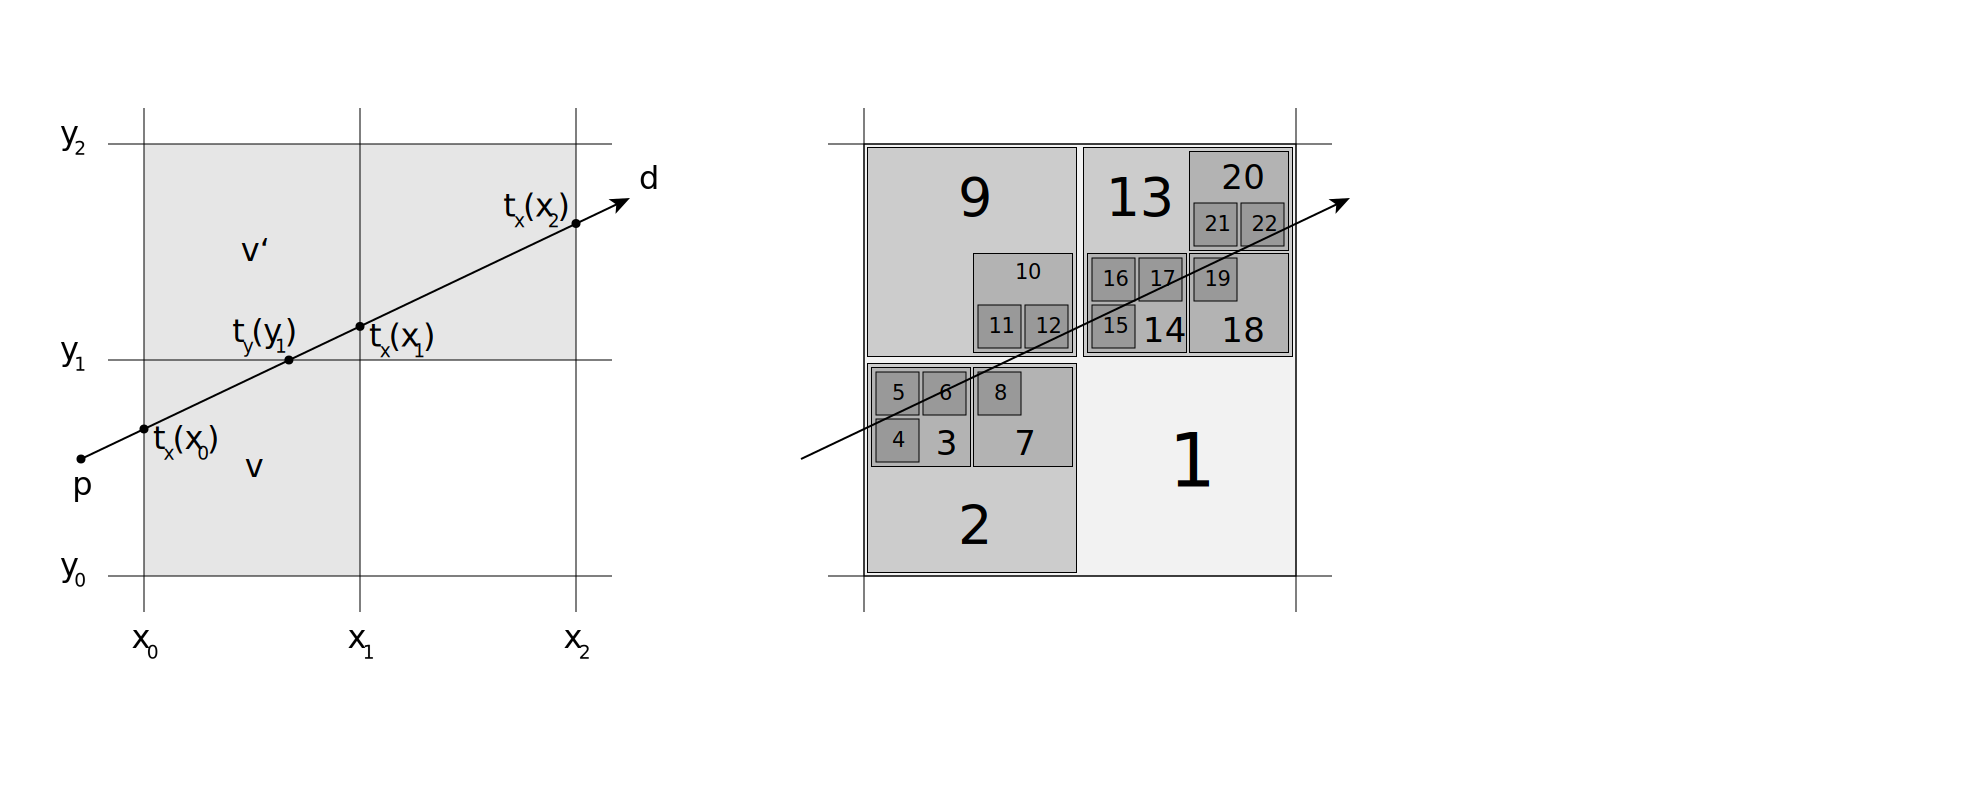
\includegraphics[width=0.75\textwidth]{figures/raycasting.pdf}
  \caption{Bestimmung der Reihenfolge der Kindknoten beim Schnitt \label{raycasting}}
\end{figure}




\subsection{Verwandte Arbeiten}


%  ////////////////////////////////////////////////////////////////////


\section{Out-of-Core Datenmanagement}
Out-of-Core-Strategien erm�glichen einer Anwendung oder einem System die Verwendung von Datenmengen, welche die lokale Speicherkapazit�t �bersteigen. Voraussetzung daf�r ist die Seg\-men\-tier\-bar\-keit der Daten. Au�erdem muss die lokal gespeicherte Untermenge der segmentierten Daten zu jedem Zeitpunkt zur Verarbeitung gen�gen.
\begin{figure}[position=h]
  \centering
  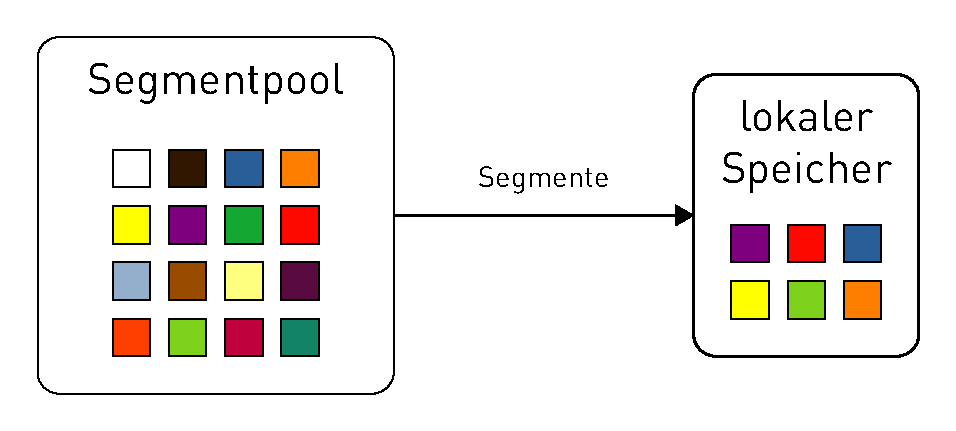
\includegraphics[width=0.75\textwidth]{figures/out_of_core_principal.pdf}
  \caption{Out-Of-Core-Prinzip\label{out_of_core_principal}}
\end{figure}
\\
Die endliche Menge lokalen Speichers der GPU begrenzt die maximale Aufl�sung von SVO-Strukturen. Eine Vergr��erung des Speichers l�st das Problem nicht nachhaltig. Wie oben beschrieben ben�tigt jede weitere SVO-Tiefe etwa die vierfache Speicher\-menge.\\
(!!! streaming system notwendig)\\
(beispiele f�r ooc Systeme)\\

\subsection{Verwandte Arbeiten}


%  ////////////////////////////////////////////////////////////////////





\newpage
\chapter{Systemkonzeption}



%/////////////////////////////////////////////////////////



\section{�berblick}

 - Fehler bei der Darstellung -> Fehlerwert ausnutzen\\
 - Visueller/Progressiver Ansatz (outputsensitiv)\\
 - Problem bei Visuellen Ansatz: Mann muss das was man sieht einordnen k�nnen


\section{Out-of-Core Management}



%/////////////////////////////////////////////////////////



\subsection{Aufbau}


\begin{figure}[position=h]
  \centering
  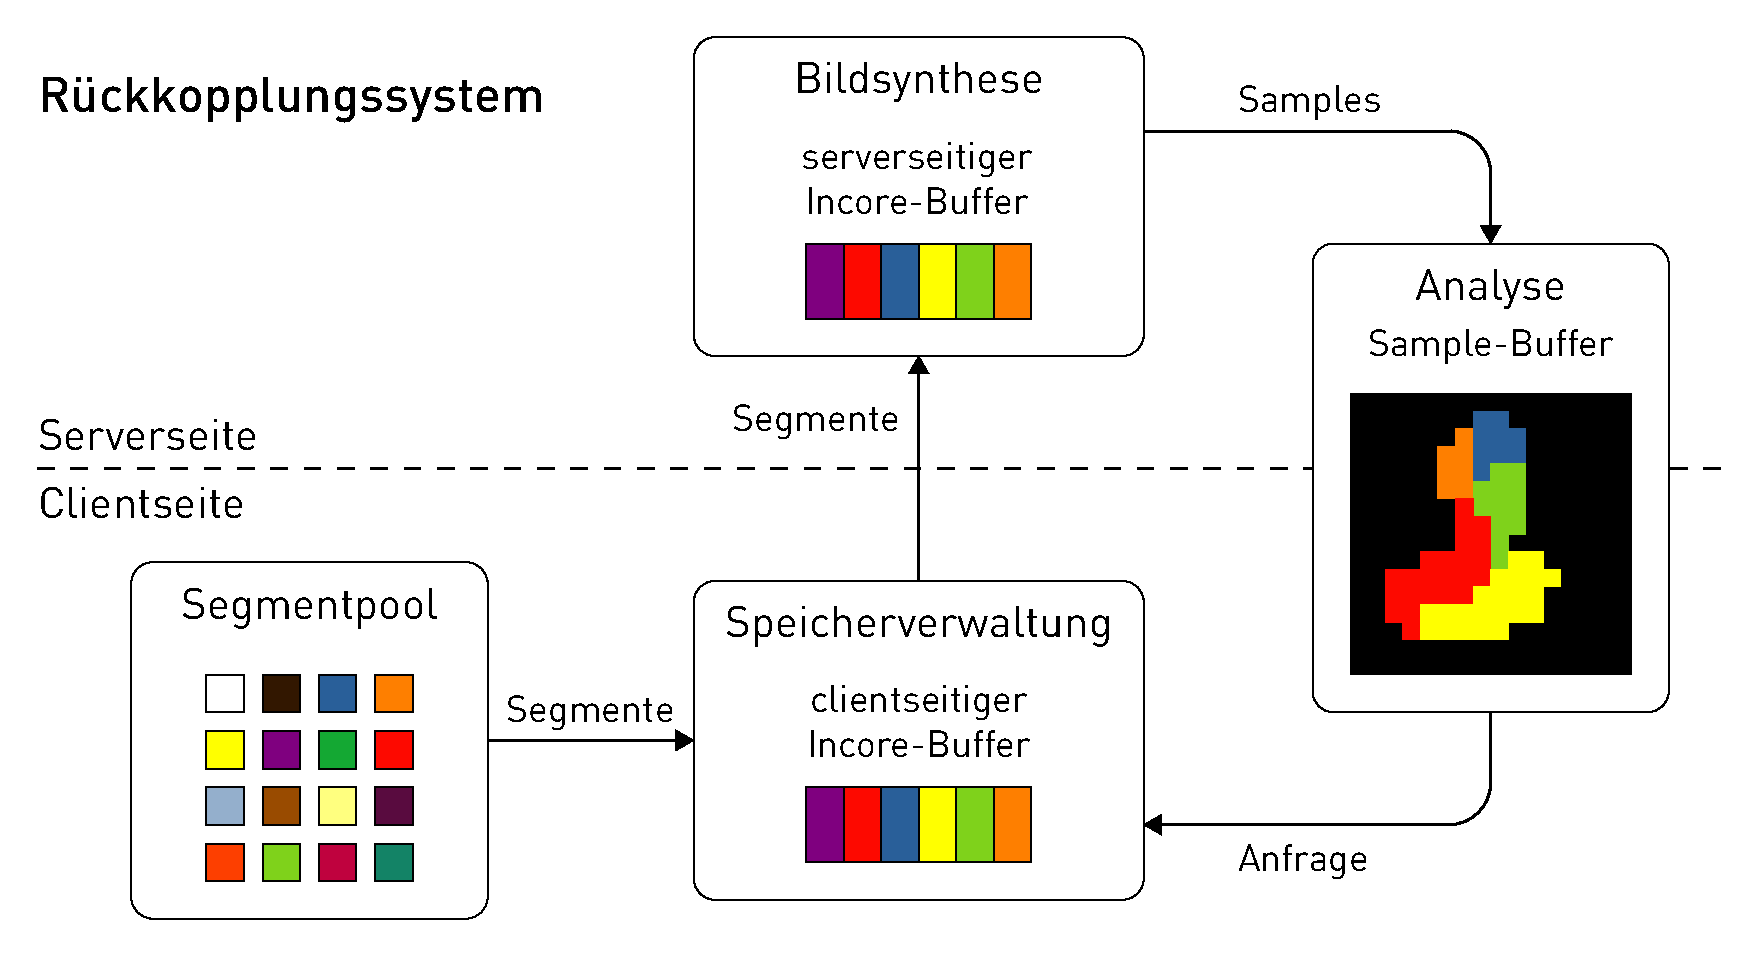
\includegraphics[width=0.85\textwidth]{figures/out-of-core_setup.pdf}
  \caption{Schematischer Aufbau des Out-Of-Core-Systems\label{out-of-core_setup1}}
\end{figure}



%/////////////////////////////////////////////////////////

\section{Datenstrukturen}


\subsection{Definition der Knotenstruktur}

Die Octree-Struktur in dieser Arbeit ist so aufgebaut, dass jeder Knoten im Baum einen Voxel repr�sentiert. Jedes Voxel steht f�r einen achsen\-parallelen W�rfel, der die Oberfl�che der abzubildenden Geometrie schneidet. Jedes Voxel kann in bis zu acht weitere Voxel unterteilt werden. Die Indizierung der Kind-Voxel ergibt sich aus ihrer Position innerhalb des Eltern-Voxels. Diese kann durch die Vorschrift \textbf{$i(x,y,z)=4p(x)+2p(y)+p(z)$} bestimmt werden, wobei $p(x)$, $p(y)$ und $p(z)$ f�r die Ergebnisse der Aussagen $x>0$, $y>0$ und $z>0$ stehen. Abbildung \ref{voxel_idx} zeigt ein vollst�ndig unterteiltes Voxel und die Indizierung seiner Kind-Voxel.
\begin{figure}[position=h]
  \centering
  \includegraphics[width=0.35\textwidth]{figures/voxel_idx.pdf}
  \caption{Indizierung der Kind-Voxel\label{voxel_idx}}
\end{figure}\\
Die Topologie des Octrees wird durch 64 Bit gro�e Knoten beschrieben. Der Speicherbedarf teilt sich in 32 Bit f�r den Verweis auf das erste Kind (\textbf{\textit{First-Child-Index}}) und zwei Bitmasken, die jeweils 8 Bit beanspruchen. Eine Bitmaske kodiert in jedem Bit das jeweilige Vorhandensein eines Kindes (\textbf{\textit{Valid-Mask}}). Die zweite Bitmaske kodiert in jedem Bit ob das jeweilige Kind ein Blatt ist oder nicht (\textbf{\textit{Leaf-Mask}}). Abbildung \ref{node_struktur} veranschaulicht den Aufbau der Baumstruktur durch diese Knoten\-repr�sentation.
\begin{figure}[position=h]
  \centering
  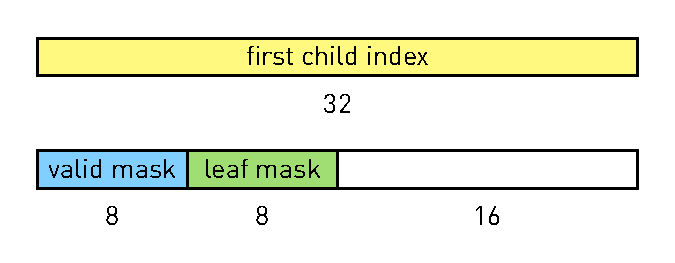
\includegraphics[width=0.5\textwidth]{figures/node_memory.pdf}
  \caption{Aufbau eines Knotens\label{node_memory}}
\end{figure} 
16 Bit pro Knoten bleiben f�r die Anwendung in dieser Arbeit frei. Der freie Platz ist mit den Anforderungen an minimale Speichergr��en und Segmentierung der OpenCL zu erkl�ren, die keine 24 oder 48 Bit Datentypen definiert. Es ist jedoch m�glich, diesen Platz zum Speichern von Attributen oder Verweisen zu Kontur\-informationen zu nutzen, wie es in (ESVOR) getan wird. L�sungsvorschl�ge f�r eine kompaktere Notation werden in diskutiert.
\begin{figure}[position=h]
  \centering
  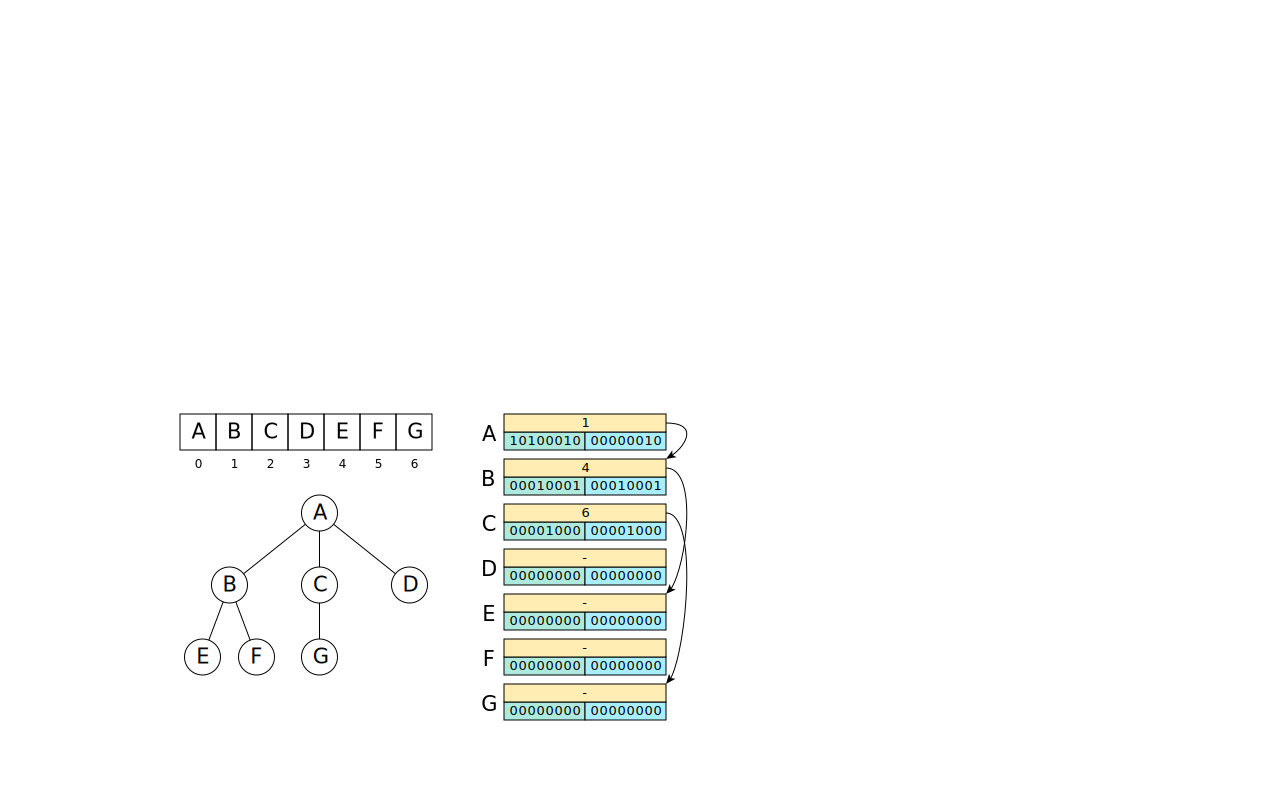
\includegraphics[width=0.55\textwidth]{figures/node_struktur.pdf}
  \caption{Beschreibung der SVO-Struktur\label{node_struktur}}
\end{figure}

%/////////////////////////////////////////////////////////

\newpage

\subsection{Segmentierung}\label{sec:segmentierung}
Bei der Wahl der Speichergr��e der Segmente gilt es zwischen Granularit�t und Aufwand abzuw�gen. Um eine hohe Granularit�t und damit eine hohe Anpassungsf�higkeit der gew�hlten Untermenge an Segmenten zu gew�hrleisten, sollte die Gr��e der Segmente eher klein gew�hlt werden. Sind die Segmente jedoch zu klein k�nnen f�r einen gegebenen Octree schnell mehrere Millionen davon entstehen, was den Verwaltungsaufwand erh�ht. Zu gro�e Segmente k�nnen dazu f�hren das einzelne Operationen auf Segmenten zu viel Zeit ben�tigen und damit das Gesamtsystem ausbremsen.\\
Die Unterteilung der SVO-Struktur in dieser Arbeit erfolgt in Unterb�umen die als \textit{Treelets} (B�umchen) bezeichnet werden sollen. Jedes Treelet umfasst die gleiche Anzahl an Knoten und stellt f�r sich gesehen einen Sparse Voxel Octree mit Wurzel- und Blatt\-knoten dar (vgl. Abbildung \ref{treelet_struktur}). Bei initialen Test haben sich Treelet-Gr��en zwischen einem und zw�lf Kilobyte als g�nstig erwiesen. Im Abschnitt \ref{sec:test_einfluss_groesse} (\nameref{sec:test_einfluss_groesse}) wird der Einflu� dieser Gr��e untersucht. Zum Identifizieren eines Treelets erh�lt jedes einen eindeutigen Index (\textit{Treelet-Index}). �ber diesen wird die Verkn�pfung der Treelets untereinander realisiert. Dazu speichert jedes Treelet unter anderem den Index des �bergeordneten Treelets und die Position des ihm entsprechenden Blattknotens.
Die im Baum abw�rts gerichtete Verkn�pfung wird durch Speichern der Indices der untergeordneten Treelets im First-Child-Index des je\-wei\-ligen Blattknotes realisiert.
\begin{figure}[position=h]
  \centering
  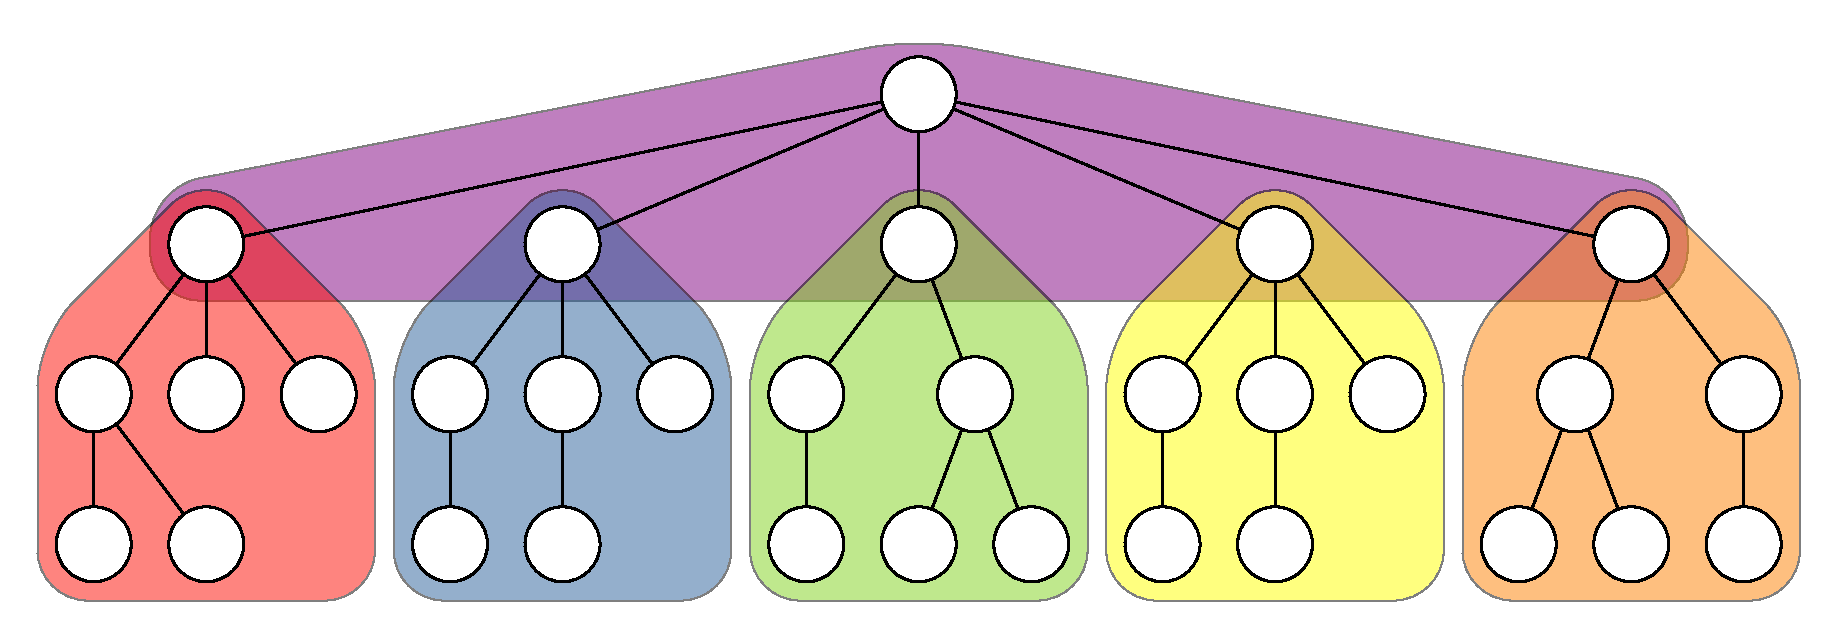
\includegraphics[width=0.75\textwidth]{figures/treelet_struktur.pdf}
  \caption{Treelet-Struktur mit 6 Knoten pro Treelet \label{treelet_struktur}}
\end{figure}
\newpage
Die Verbindung der Treelets untereinander bildet einen bidirektionalen Baum �ber dem eigentlichen Octree. Abbildung \ref{verbinung_ueber_treelet_index} stellt diese Verbindung dar. Unter der Abbildung des Baumes sind die Werte der First-Child-Pointer f�r alle Knoten notiert. Durch die abw�rts gerichtete Verbindung, die in den Blatt-Knoten gespeichert ist, kann beim Traversieren der Struktur in jedem Blatt das zugeh�rige Treelet ermittelt werden. Die aufw�rts gerichtete Verbindung erm�glicht den effizienten Zugriff auf alle �bergeordneten Treelets bis zum Wurzel-Treelet. Dies sind die Treelets, von denen ein gegebenes Treelet f�r seine Verarbeitung in der SVO-Struktur abh�ngig ist.
\begin{figure}[position=h]
  \centering
  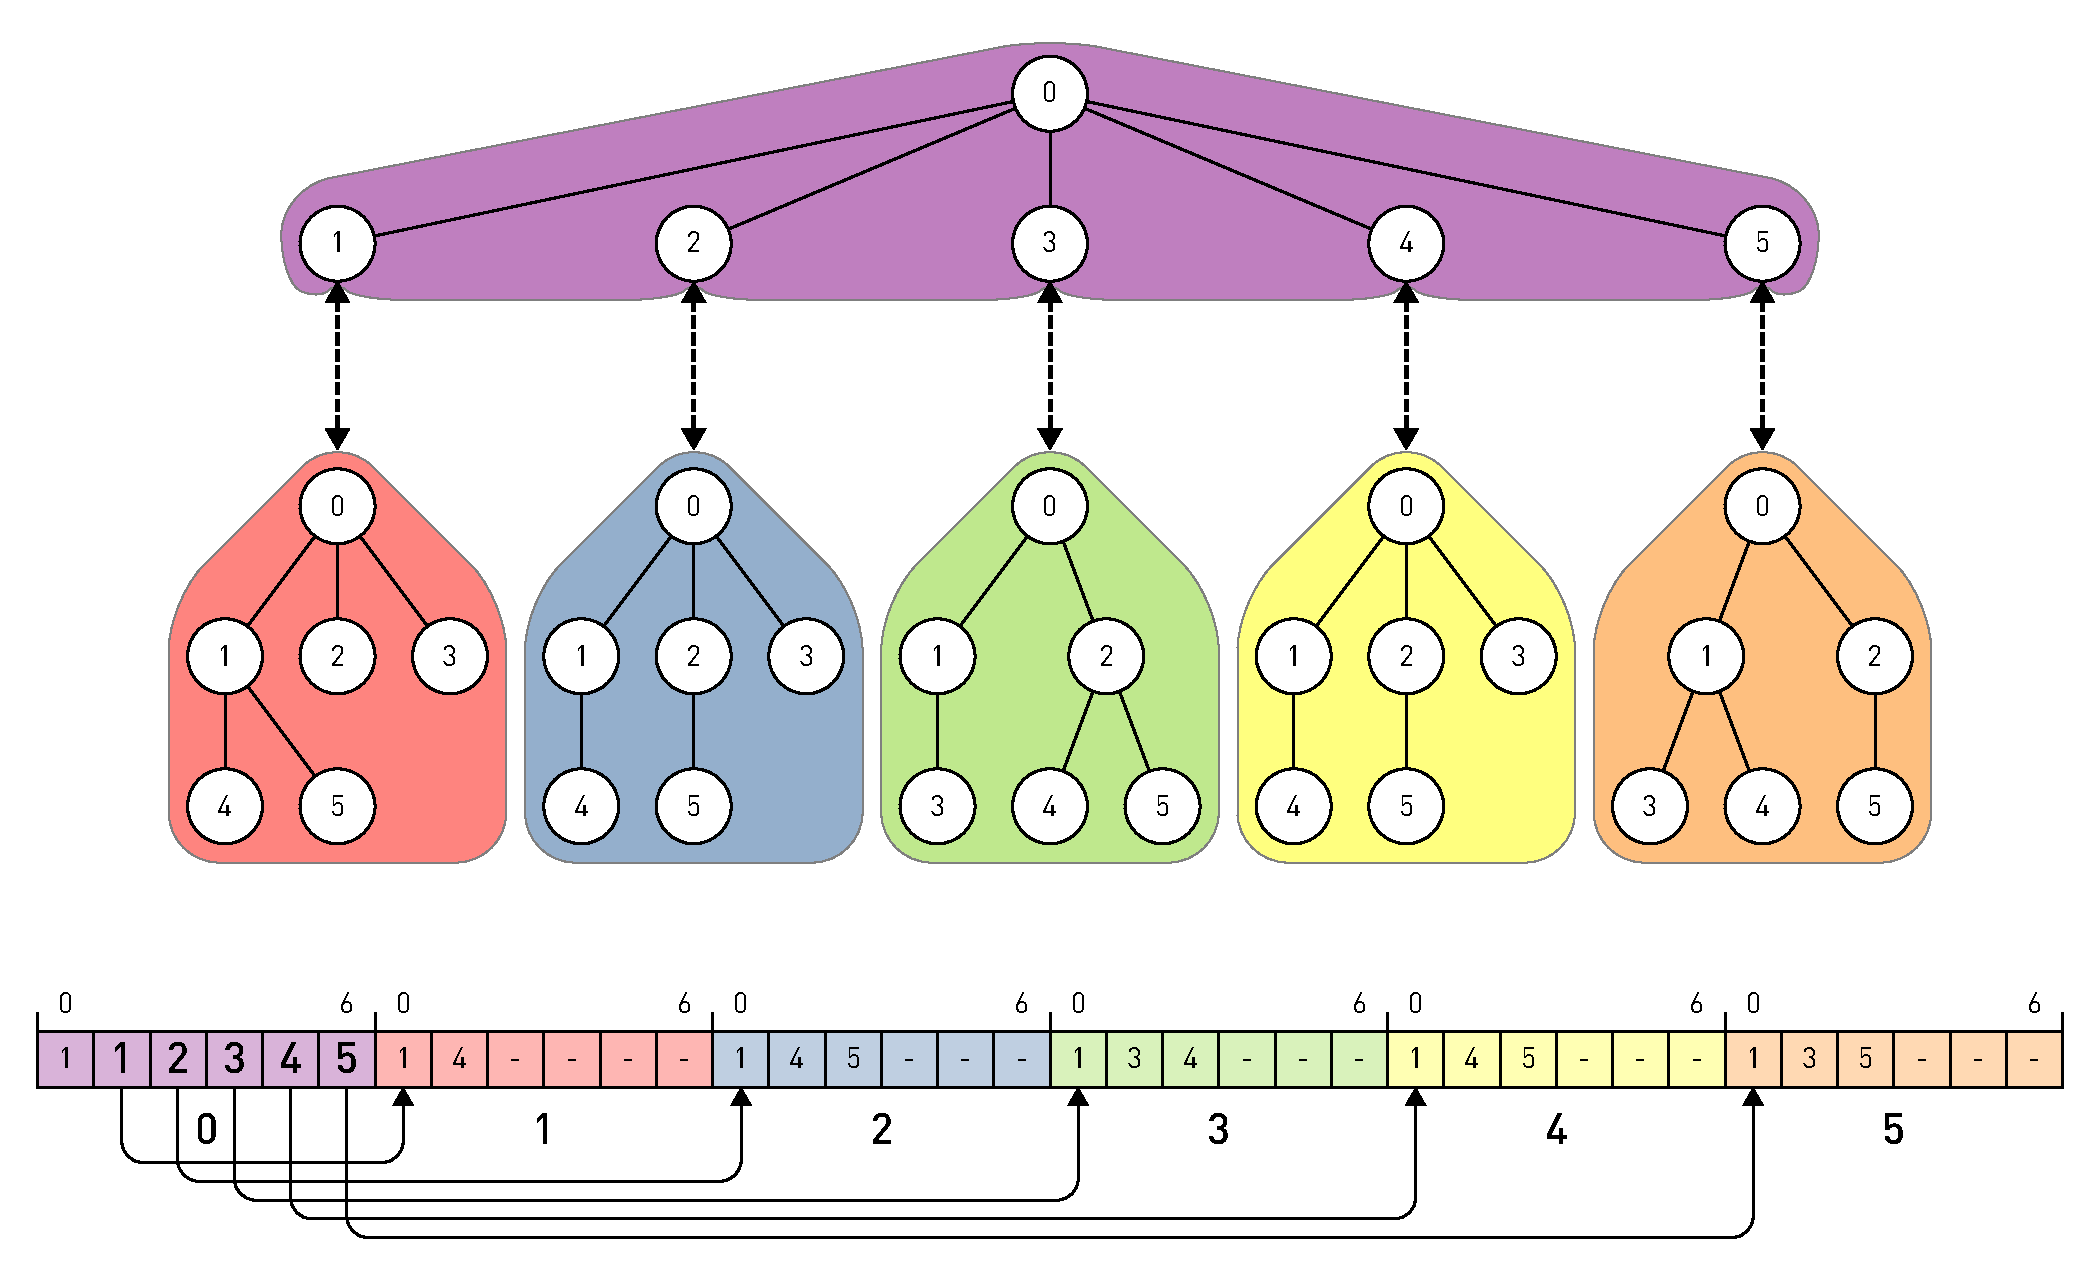
\includegraphics[width=0.90\textwidth]{figures/verbinung_ueber_treelet_index.pdf}
  \caption{Verbindung der Treeelets durch ihren Index \label{verbinung_ueber_treelet_index}}
\end{figure}
\newline 


%/////////////////////////////////////////////////////////


\newpage
\subsection{Attribute}\label{sec:attribute}

Attributinformationen werden parallel zu den Treelets in einem oder mehreren Attribut-Buffern gehalten. Diese Buffer k�nnen, wie auch die Knotenstruktur des Octrees, sehr gro� werden da ben�tigte Attributwerte f�r jedes Voxel des Octrees einzeln gespeichert werden. Darum werden die Werte, wie Beleuchtungsinformationen, Farben, Richtungsinformationen oder ambiente Verdeckungswerte (Ambient Occlusion) vor dem Ablegen komprimiert. Dies kann durch die Verwendung von 8 Bit-Datentypen f�r die einzelnen Attribut-Komponenten geschehen.
\begin{figure}[position=h]
  \centering
  \includegraphics[width=0.75\textwidth]{figures/interleaved_attributes.png}
  \caption{Attribut-Buffer mit verschachtelten Farb- und Richtungswerten  \label{interleaved_attributes}}
\end{figure}



%/////////////////////////////////////////////////////////


\newpage
\section{Generalisiertes System zur Erstellung von Sparse Voxel Octrees}
Das System zur Erstellung der SVO-Struktur ist modular aufgebaut und besteht prinzipiell aus drei Teilen: Dem \textbf{\textit{Build-Manager}} der den Ablauf der SVO-Generierung steuert, einem \textbf{\textit{Treelet-Builder}} der die Treelets erstellt und abh�ngig vom Typ der Eingabedaten gew�hlt wird und einem \textbf{\textit{Attributgenerator}} der in Abh�ngig von Eingabedaten und gew�nschter Attributkonfiguration der Ausgabedaten gew�hlt werden kann. Mit dieser Unterteilung des Systems ist es prinzipiell m�glich, unterschiedliche Eingabedaten wie 3D-Objekte aus Dreiecksnetzen oder Punktwolken zu verarbeiten und eine Vielzahl von Attribut\-konfigurationen zu erstellen. Durch den modularen Aufbau und die Bereitstellung entsprechender Basisklassen ist es m�glich, Unterst�tzung f�r weitere Eingabeformate zu schaffen.
\begin{figure}[position=h]
  \centering
  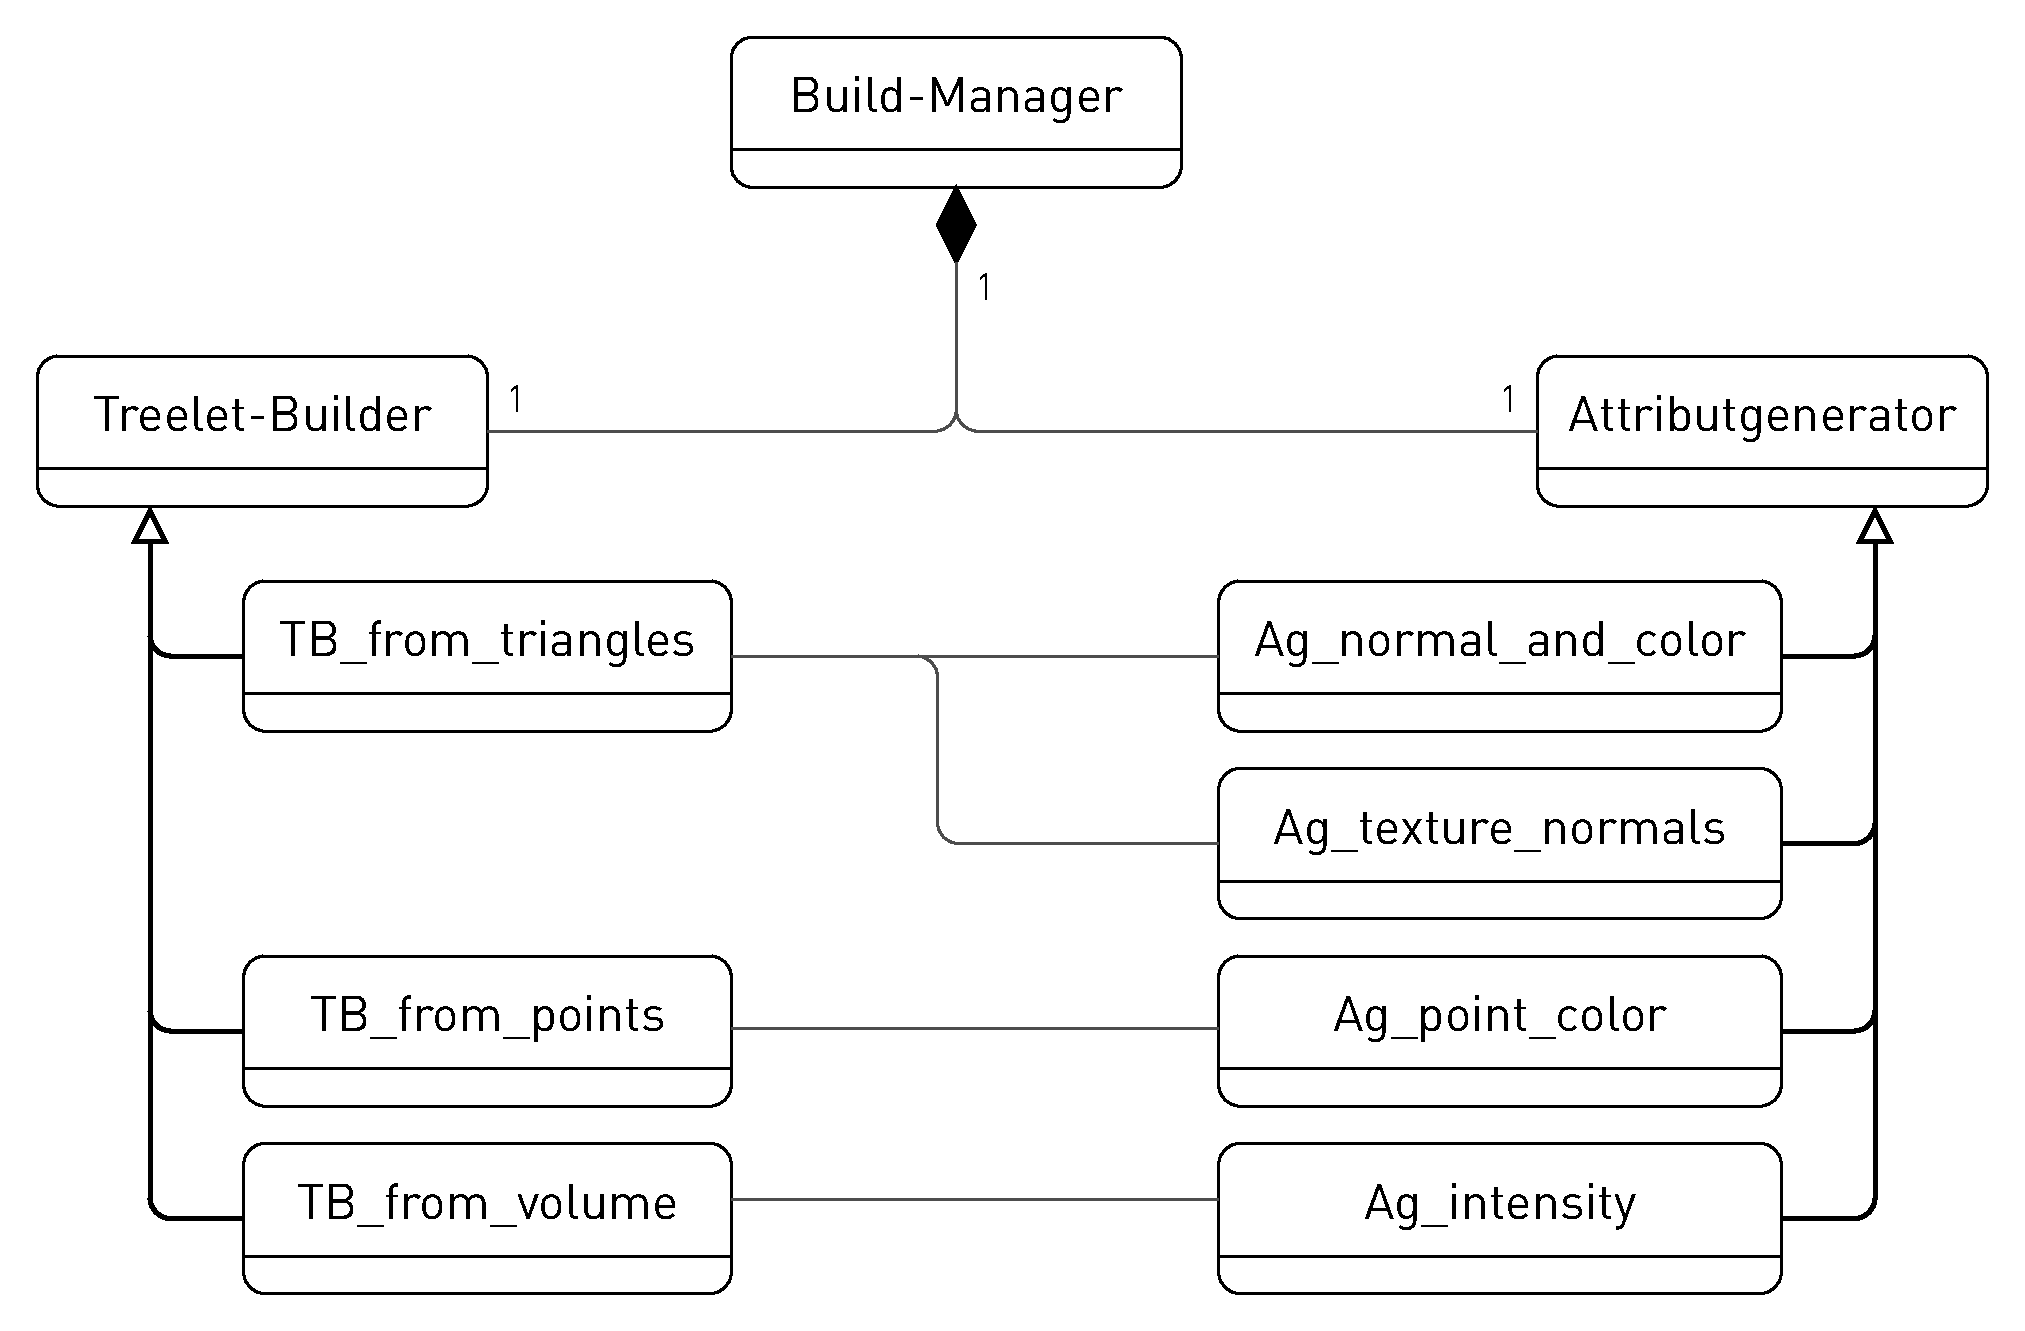
\includegraphics[width=0.75\textwidth]{figures/uml.pdf}
  \caption{Klassendiagram des generallisierten Erstellungssystems \label{uml_diagam}}
\end{figure}
Das in Abbildung \ref{uml_diagam} gezeigte Klassen\-diagramm stellt die Relationen zwischen den einzelnen Komponenten dar. Der Build-Manager besitzt einen Treelet-Builder der abh�ngig von der Art der Eingabedaten gew�hlt wird. Dazu besitzt er einen passenden Attributgenerator der anhand der Eingabedaten und SVO-Repr�sentation Attribute f�r alle Knoten erzeugt.

%/////////////////////////////////////////////////////////

\section{Verwendete Infrastruktur}
gloost
opencl
bencl
%/////////////////////////////////////////////////////////

\section{Client-Server-Architektur}
Es kommt darauf an wer die Anfragen stellt, nicht wer die Daten h�lt.


%/////////////////////////////////////////////////////////




\section{Real Time Rendering von Sparse Voxel Octrees}


\newpage
\chapter{Implementierungsdetails und Umsetzung}


\section{�berblick}

\newpage

\section{Aufbau der SVO Datenstruktur}


\subsection{Definition der Knotenstruktur}

Die Octree-Struktur in dieser Arbeit ist so aufgebaut, das jeder Knoten im Baum einen Voxel repr�sentiert. Jeder Voxel steht f�r einen achsen\-paralleler W�rfel der die Oberfl�che der abzubildenden Geometrie schneidet. Jeder Voxel kann in bis zu acht weitere Voxel unterteilt werden. Die Indizierung der Kind-Voxel ergibt sich aus ihrer Position innerhalb des Eltern-Voxels. Diese kann durch die Vorschrift \textbf{$i(x,y,z)=4p(x)+2p(y)+p(z)$} bestimmt werden, wobei $p(x)$, $p(y)$ und $p(z)$ f�r die Ergebnisse der Aussagen $x>0$, $y>0$ und $z>0$ stehen. Abbildung \ref{voxel_idx} zeigt ein vollst�ndig unterteilten Voxel und die Indizierung seiner Kind-Voxel.
\begin{figure}[position=h]
  \centering
  \includegraphics[width=0.35\textwidth]{figures/voxel_idx.pdf}
  \caption{Indizierung der Kind-Voxel\label{voxel_idx}}
\end{figure}\\
Die Topologie des Octrees wird durch 64 Bit gro�e Knoten beschrieben. Der Speicherbedarf teilt sich in 32 Bit f�r den Verweis auf das erste Kind (\textbf{\textit{First-Child-Index}}) und zwei Bitmasken, die jeweils 8 Bit beanspruchen. Eine Bitmaske kodiert in jedem Bit das jeweilige Vorhandensein eines Kindes (\textbf{\textit{Valid-Mask}}). Die zweite Bitmaske kodiert in jedem Bit ob das jeweilige Kind ein Blatt ist oder nicht (\textbf{\textit{Leaf-Mask}}). Abbildung \ref{node_struktur} veranschaulicht den Aufbau der Baumstruktur durch diese Knoten\-repr�sentation. 
16 Bit pro Knoten bleiben f�r die Anwendung in dieser Arbeit frei, k�nnen aber auf verschiedene Weise genutzt werden. Beispielsweise ist es m�glich diesen Platz zum Speichern von Attributen oder Verweisen zu Kontur\-informationen zu nutzen, wie es in (ESVOR) getan wird. Der freie Platz ist mit den Anforderungen an minimale Speichergr��en und Segmentierung der OpenCL zu erkl�ren, die keine 24 oder 48 Bit Datentypen definiert. L�sungsvorschl�ge f�r eine kompaktere Notation werden in ( !!! verweis auf verbesserungen) diskutiert.
\begin{figure}[position=h]
  \centering
  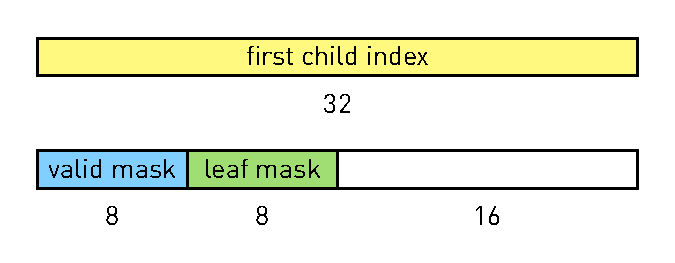
\includegraphics[width=0.55\textwidth]{figures/node_memory.pdf}
  \caption{Aufbau eines Knotens\label{node_memory}}
\end{figure}
\begin{figure}[position=h]
  \centering
  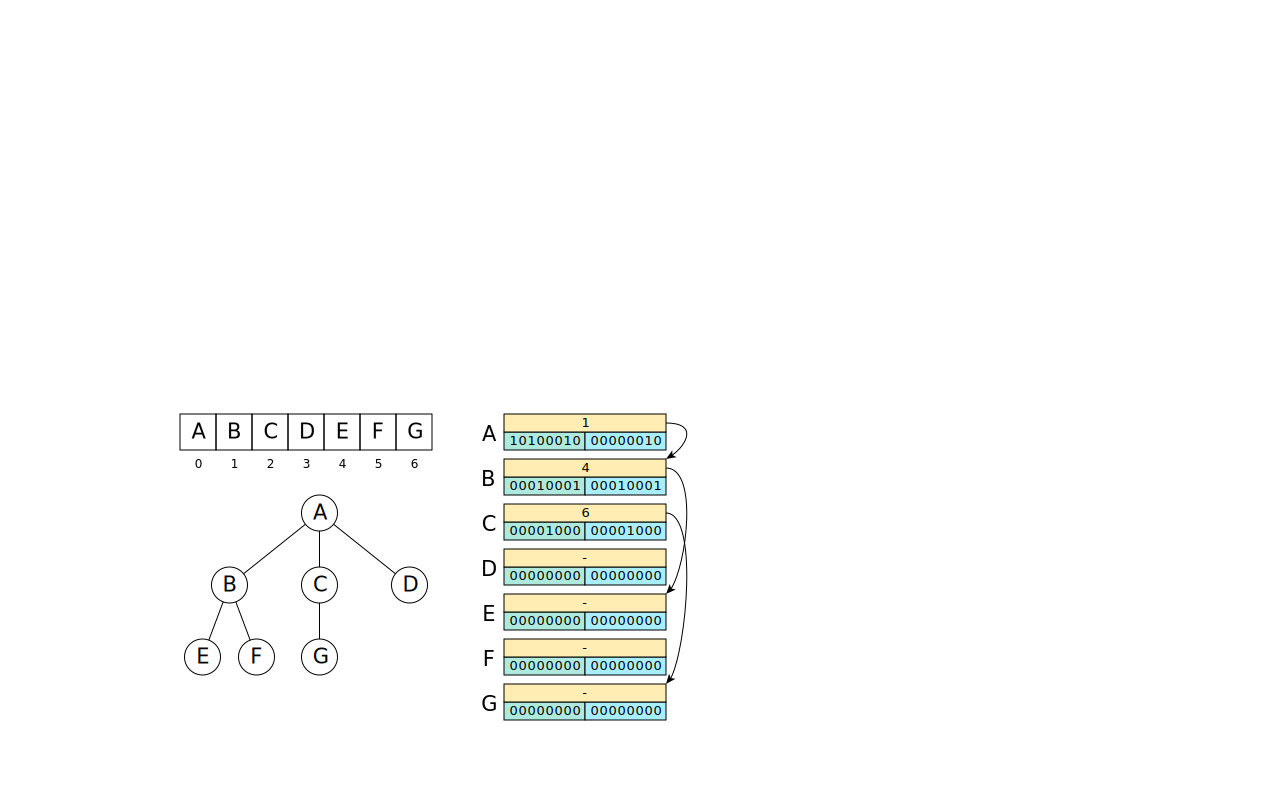
\includegraphics[width=0.55\textwidth]{figures/node_struktur.pdf}
  \caption{Beschreibung der SVO-Struktur\label{node_struktur}}
\end{figure}



%/////////////////////////////////////////////////////////



\subsection{Segmentierung}\label{sec:segmentierung}

\begin{figure}[position=h]
  \centering
  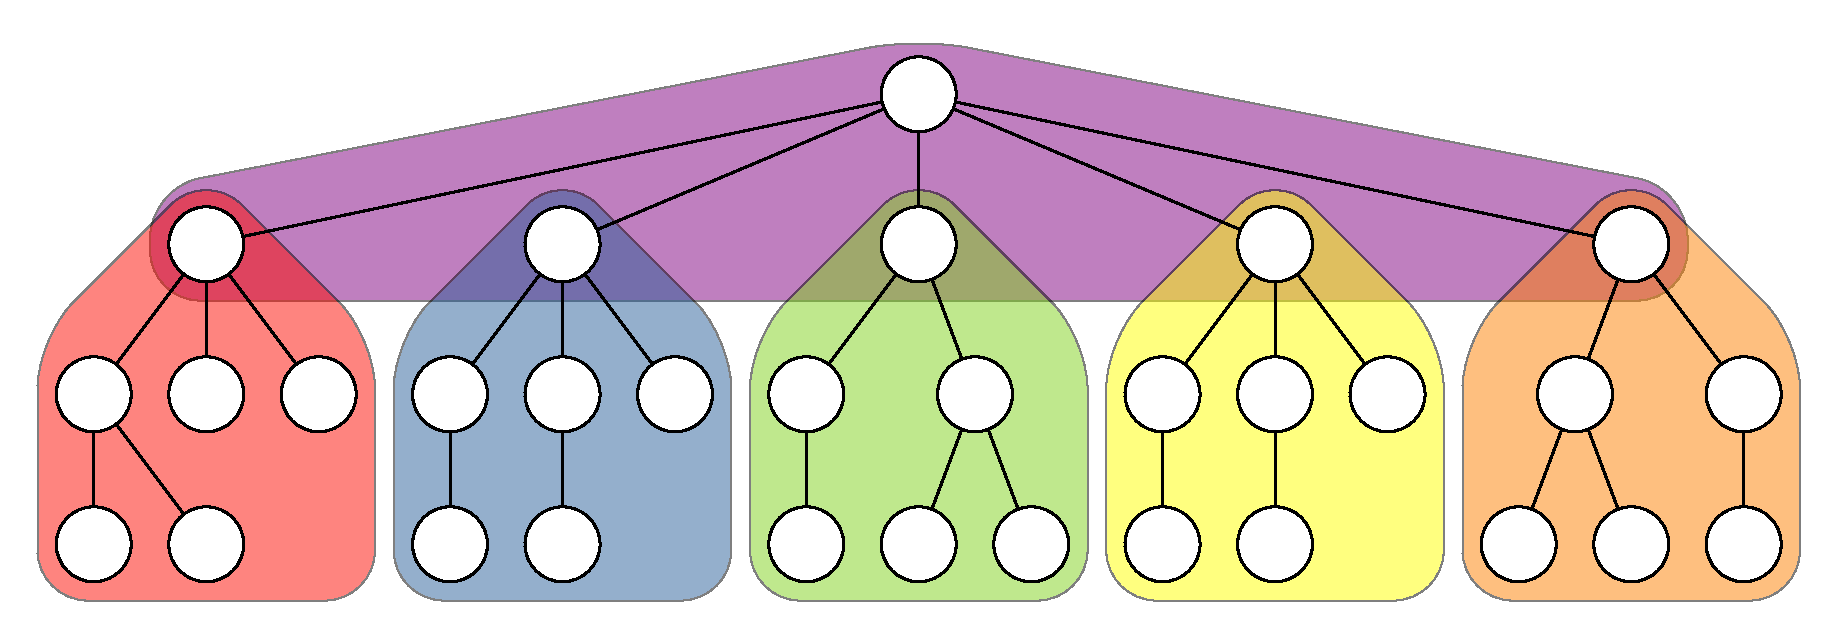
\includegraphics[width=0.75\textwidth]{figures/treelet_struktur.pdf}
  \caption{Treelet-Struktur mit 6 Knoten pro Treelet \label{treelet_struktur}}
\end{figure}
Die Unterteilung der SVO-Struktur erfolgt in Unterb�umen die in dieser Arbeit als \textit{Treelets} (B�umchen) bezeichnet werden. Jedes Treelet umfasst die selbe Anzahl an Knoten und stellt f�r sich gesehen einen Sparse Voxel Octree, mit Wurzel- und Blatt\-knoten dar (vgl. Abbildung \ref{treelet_struktur}). Zum Identifizieren eines Treelets erh�lt jedes einen eindeutigen Index (\textit{Treelet-Index}). �ber diesen wird die Verkn�pfung der Treelets untereinander realisiert. Dazu speichert jedes Treelet den Index seines �bergeordnet Treelets und die Position des jeweiligen Blattknotens.
Die im Baum abw�rts gerichtete Verkn�pfung wird durch Speichern der Indices der untergeordneten Treelets im First-Child-Index des je\-wei\-ligen Blattknotes realisiert.
\begin{figure}[position=h]
  \centering
  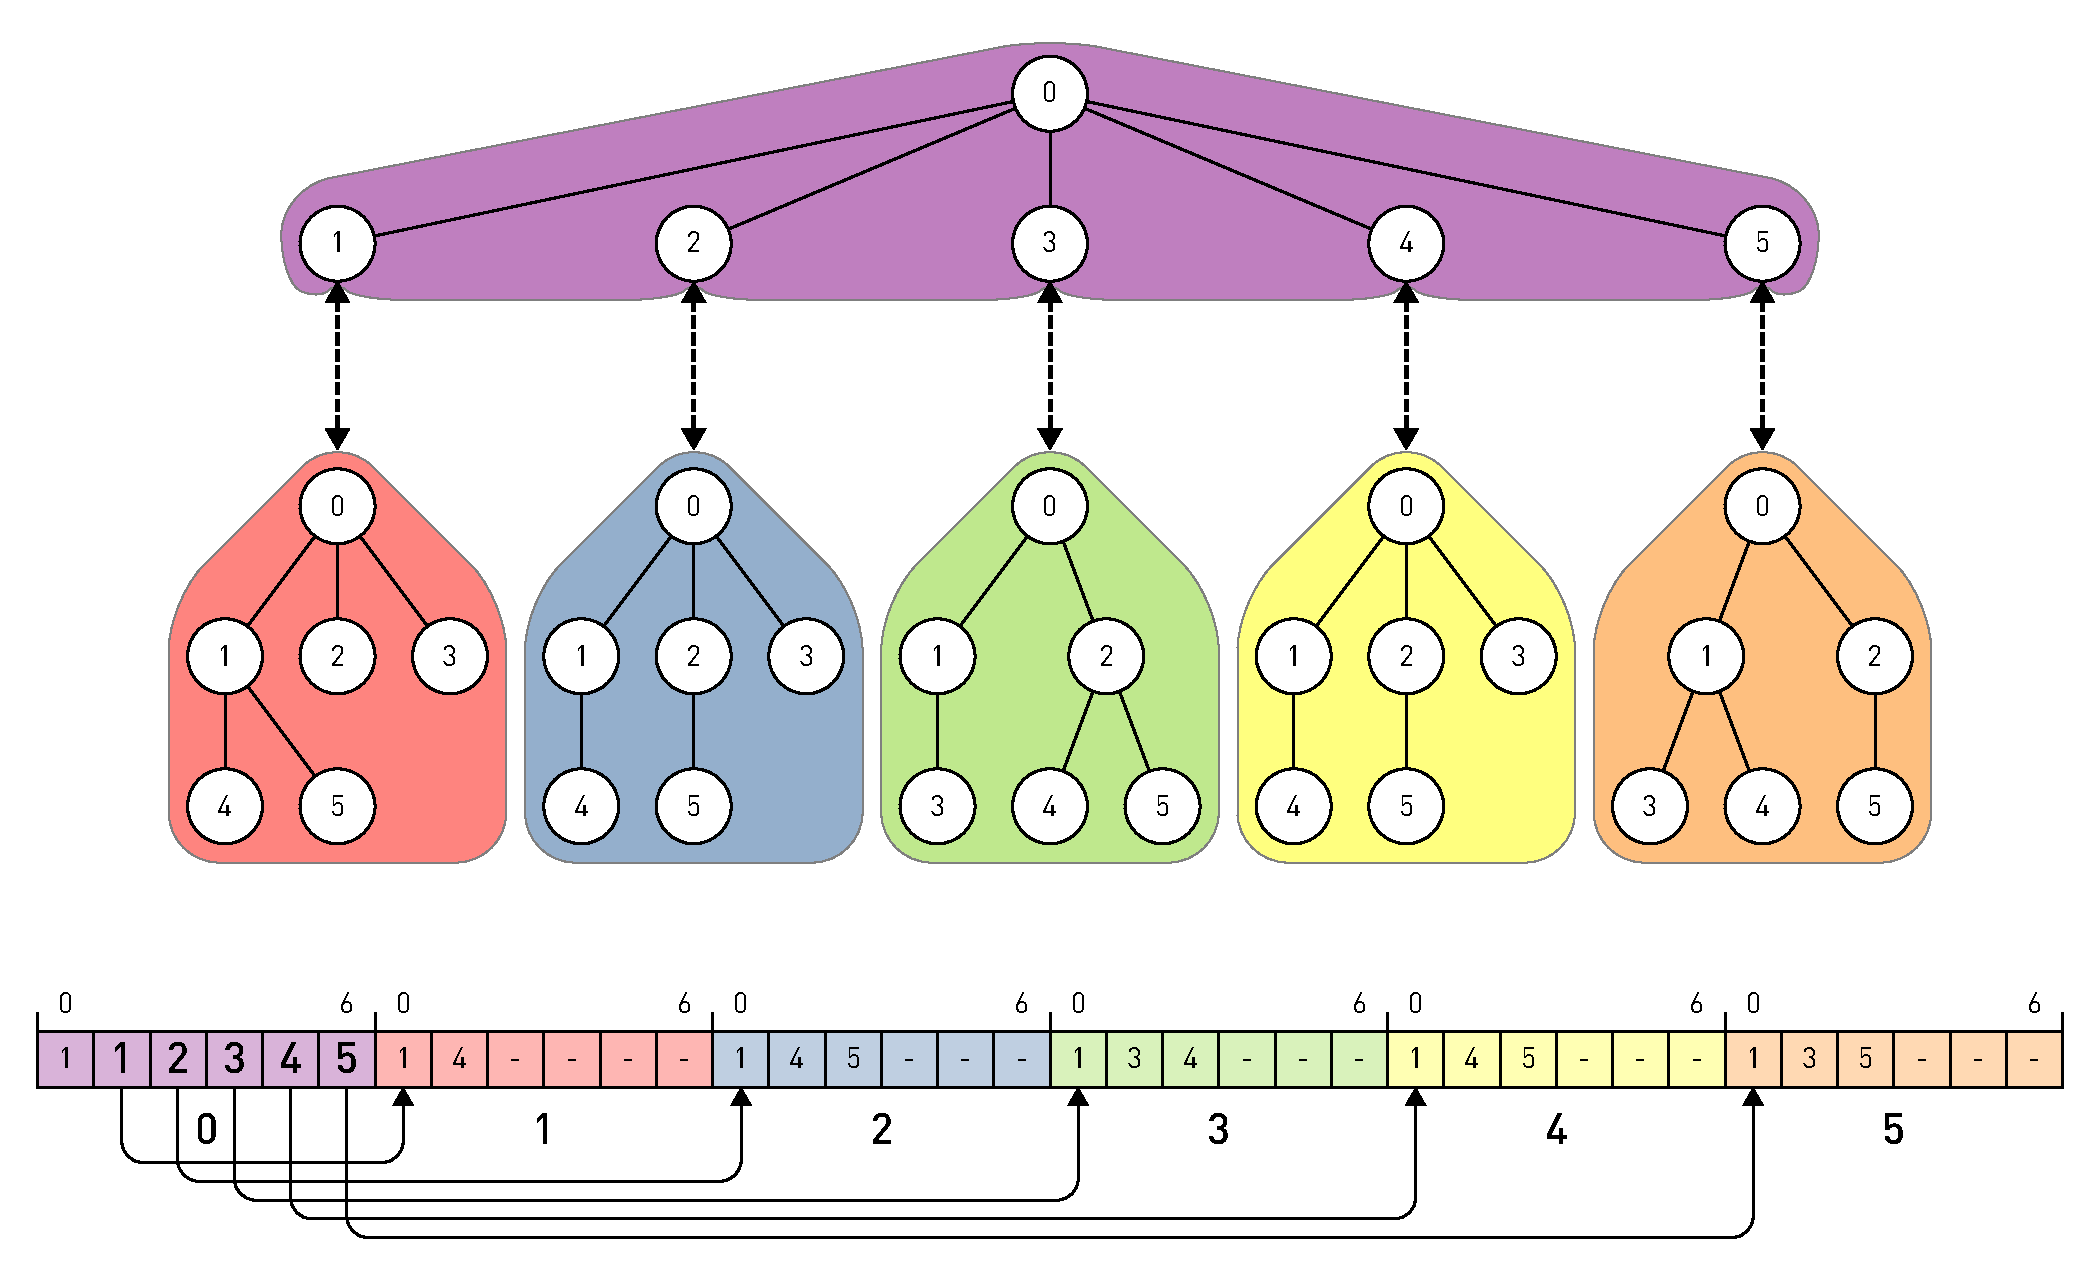
\includegraphics[width=0.90\textwidth]{figures/verbinung_ueber_treelet_index.pdf}
  \caption{Verbindung der Treeelets durch ihren Index \label{verbinung_ueber_treelet_index}}
\end{figure}
Die Verbindung der Treelets untereinander bildet einen bidirektionalen Baum �ber dem eigentlichen Octree. Abbildung \ref{verbinung_ueber_treelet_index} stellt diese Verbindung dar. Unter der Abbildung des Baumes sind Werte der First-Child-Pointer f�r alle Knoten notiert.\\
Durch die abw�rts gerichtete Verbindung, die in den Blatt-Knoten gespeichert ist kann beim Traversieren der Struktur in jedem Blatt das zugeh�rige Treelet ermittelt werden um dieses bei Bedarf anzufordern. Die aufw�rts gerichtete Verbindung erm�glicht den effizienten Zugriff auf alle �bergeordneten Treelets bis zum Wurzel-Treelet von denen ein gegebenes Treelet f�r seine Verarbeitung in der SVO-Struktur abh�ngig ist.
\newline
Die Speichergr��e der Treelets kann bei der Erstellung des Baumes angegeben werden. F�r die Tests in dieser Arbeit wurden Gr��en zwischen einem und zehn Kilobyte gew�hlt. Dabei gilt es bei der Wahl der Speichergr��e zwischen Granularit�t und Aufwand abzuw�gen  Um eine hohe Granularit�t und damit eine hohe Anpassung der gew�hlten Untermenge an Segmenten zu gew�hrleisten, sollte die Gr��e der Treelets eher klein gew�hlt werden. Sind die Treelets jedoch zu klein k�nnen f�r einen gegebenen Octree schnell mehrere Millionen Treelets entstehen. Deshalb ist es n�tig f�r jeden als Treelet-Struktur abzubildende Datensatz eine geeignete Treelet-Gr��e zu w�hlen.



%/////////////////////////////////////////////////////////



\section{Attribute}\label{sec:attribute}

Attributinformationen werden parallel zu den Treelets in einem oder mehreren Attribut-Buffern gehalten. Diese Buffer k�nnen, wie auch die Knotenstruktur des Octree, sehr gro� werden da ben�tigte Attributwerte f�r jeden Voxel des Octrees einzeln gespeichert werden. Darum werden die Werte, z.B. Beleuchtungsinformationen wie Farben, Richtungsinformationen oder ambiente Verdeckungswerte (Ambient Occlusion) vor dem Ablegen komprimiert. Dies kann durch die Verwendung von 8 Bit-Datentypen f�r die einzelnen Attribut-Komponenten.
\begin{figure}[position=h]
  \centering
  \includegraphics[width=0.90\textwidth]{figures/interleaved_attributes.png}
  \caption{Attribut-Buffer mit verschachtelten Farb- und Richtungswerten  \label{interleaved_attributes}}
\end{figure}



%/////////////////////////////////////////////////////////



\subsection{Generalisiertes System zur SVO-Erstellung}
Das System zur Erstellung der SVO-Struktur ist modular aufgebaut und besteht prinzipiell aus drei Teilen: Dem \textbf{\textit{Build-Manager}} der den Ablauf der SVO-Generierung steuert, einem \textbf{\textit{Treelet-Builder}} der die Treelets erstellt und abh�ngig vom Typ der Eingabedaten gew�hlt wird und einem \textbf{\textit{Attributgenerator}} der in Abh�ngig von Eingabedaten und gew�nschter Attributkonfiguration der Ausgabedaten gew�hlt werden kann. Mit dieser Unterteilung des Systems ist es prinzipiell m�glich verschiedenste Eingabedaten wie 3D-Objekte aus Dreiecksnetzen oder Punktwolken zu verarbeiten und eine Vielzahl von Attribut\-konfigurationen zu erstellen. Durch den modularen Aufbau und der Bereitstellung entsprechender Basisklassen ist es m�glich Unterst�tzung f�r weitere Eingabeformate zu schaffen.
\begin{figure}[position=h]
  \centering
  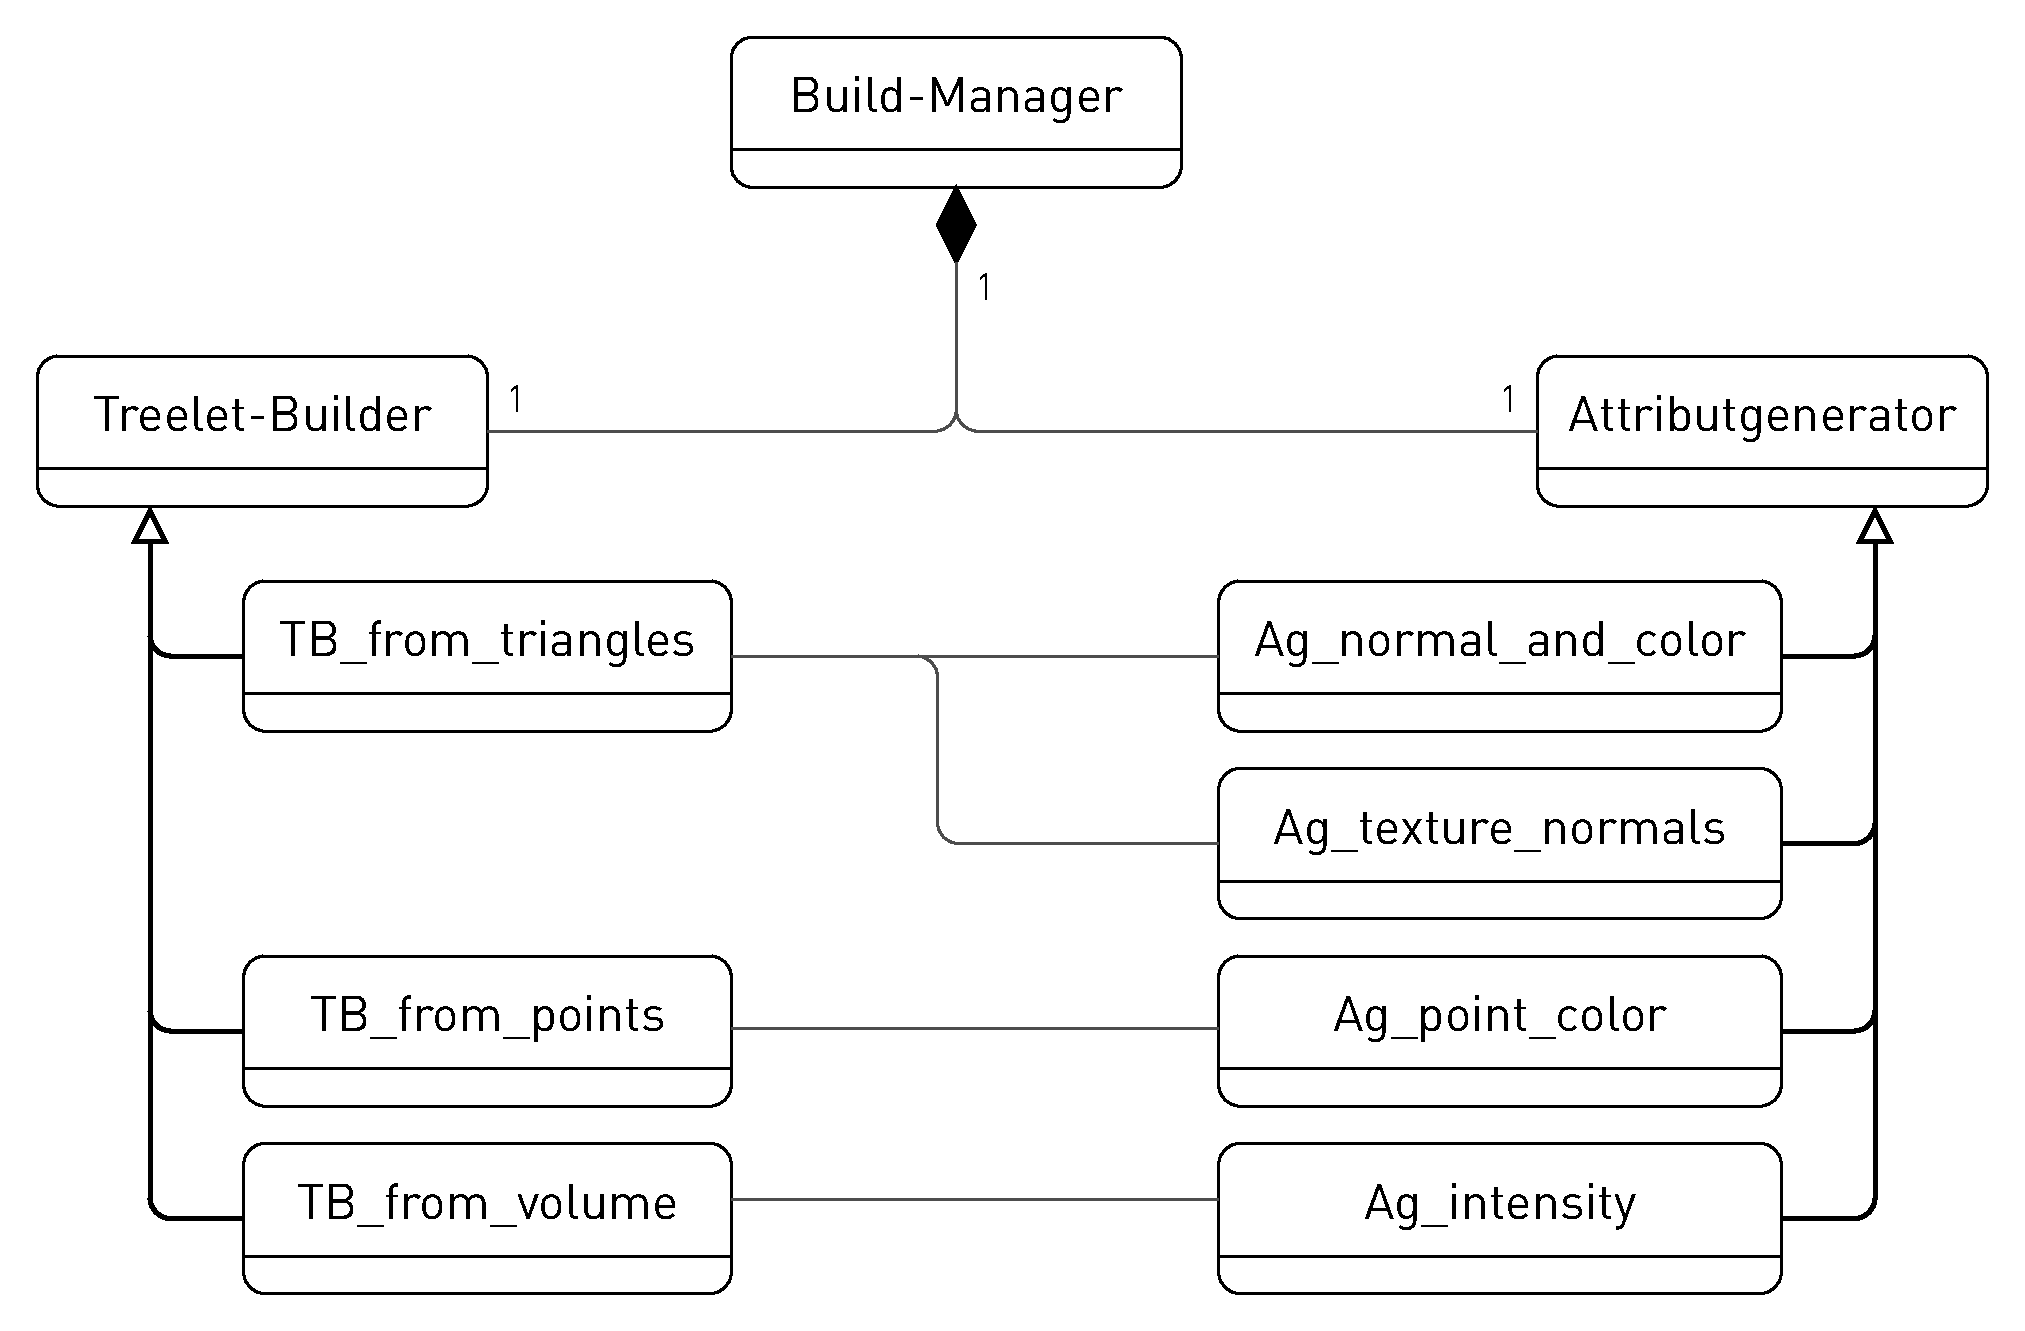
\includegraphics[width=0.75\textwidth]{figures/uml.pdf}
  \caption{Klassendiagram des generallisierten Erstellungssystems \label{uml_diagam}}
\end{figure}
Das in Abbildung \ref{uml_diagam} abgebildete Klassen\-diagramm zeigt die Relationen zwischen den einzelnen Komponenten. Der Build-Manager besitzt einen Treelet-Builder der abh�ngig von der Art der Eingabedaten gew�hlt wird. Dazu besitzt er einen passenden Attributgenerator der anhand der Eingabedaten und SVO-Repr�sentation Attribute f�r alle Knoten erzeugt.




%/////////////////////////////////////////////////////////



\subsection{Erzeugung der Treelet Struktur}\label{sec:erzeugung_treelet_struktur}

Die SVO-Struktur wird schon bei der Erstellung segmentiert, das hei�t, in Treelets unterteilt aufgebaut. Dies bietet die M�glichkeit bereits erzeugte Treelets auf die Festplatte auszulagern, sollte der Ar\-beits\-speicher nicht ausreichen um die erzeugten Daten zu halten. Im Folgendem soll ein �berblick �ber den Ablauf der Erstellung einer SVO-Struktur aus Treelets gegeben werden. In den folgenden Abschnitten werden die einzelnen Schritte genauer betrachtet.\\\\
Als Eingabe werden zun�chst die gew�nschte, minimale Tiefe des resultierenden Octrees, die Speichergr��e der Treelets und der Pfad zu den Eingabedaten ben�tigt. Der Build-Manager erstellt ein initiales, leeres Treelet (\textit{Wurzel-Treelet}) und �bergibt dieses an den Treelet-Builder. Dieser f�llt das Treelet anhand der Eingabedaten. Anschlie�end werden alle entstandenen Blatt-Knoten, die noch nicht die gew�nschte, minimale Tiefe in der Octree-Struktur aufweisen, notiert. Zu jedem dieser Blattknoten wird eine Liste der in ihm liegenden Primitive der Eingabedaten gespeichert. Zus�tzlich wird auch seine Tiefe im Baum und seine Transformation relativ zum Wurzelknoten notiert. Au�erdem wird jeweils der Treelet-Index, der Index des Blattknotens und dessen Elternknotens gespeichert um die Verkn�pfung der Treelets realisieren zu k�nnen (vgl. Abschnitt \ref{sec:segmentierung} \nameref{sec:segmentierung}, Seite \pageref{sec:segmentierung}).
Der Build-Manager speichert diese Informationen in einer Queue und erzeugt f�r jeden Eintrag ein neues Treelet (\textit{Top-Down}). Diese werden durch die gespeicherten Treelet- und Blattknotenindices des Wurzel-Treelets initialisiert und sind so logisch mit diesem verbunden. Jedes dieser Treelets wird wiederum dem Treelet-Builder �bergeben, der sie anhand seiner Primitivliste und der gespeicherten Transformation f�llt. Der Build-Manager erzeugt sukzessiv weitere Treelets aus Blattknoten bereits erstellter Treelets bis die geforderte minimale Tiefe des Octrees f�r alle Blattknoten erreicht ist.
\begin{figure}[position=h]
  \centering
  \includegraphics[width=0.83\textwidth]{figures/treelet_building.pdf}
  \caption{Schrittweiser Aufbau der SVO-Struktur aus Treelets \label{fig:treelet_building}}
\end{figure}
\newpage
F�r Blattknoten mit ausreichender Tiefe erzeugt ein Attributgenerator die gew�nschten Attribute und speichert diese in einem zus�tzlichen Buffer. Die Primitiv\-liste und alle weiteren Informationen die zur Erstellung weiterer Treelets ben�tigt w�rden k�nnen an dieser Stelle verworfen werden. Abbildung \ref{fig:treelet_building} zeigt den schrittweisen Aufbau eines Octrees aus Treelets.\\
Ist die Erstellung der Treelets abgeschlossen werden die Attribute der inneren Knoten durch Mitteln der Attribute ihrer Untergeordneten Knoten erstellt. Dies geschieht f�r alle Treelets in umgekehrter Reihenfolge ihrer Erstellung (\textit{Bottom-Up}). So wird sichergestellt, dass der Wurzelknoten eines untergeordneten Treelets bereits Attributinformation enth�lt wenn sein �bergeordnetes Treelet diese zur Generierung seiner Attribute in seinen Blattknoten ben�tigt. Ist die Erstellung der Attribute bis in den Wurzelknoten des Wurzel-Treelets vorangeschritten ist die Erstellung des Octrees abgeschlossen. 




%/////////////////////////////////////////////////////////



\subsection{Treelet Aufbau}
Der Treelet-Builder erstellt die Knoten in der Breite (\textit{Breadth-First}) und arbeitet dazu intern auf einem FIFO-Kontainer (\textit{Queue}). Der Aufbau eines Elementes dieser Queue ist im Listing \ref{lst:queueelement} zu sehen. Jedes Element der Queue entspricht einem Knoten in der SVO-Struktur und enth�lt einerseits alle Informationen die n�tig sind diesen Knoten seinem �bergeordneten Knoten mitzuteilen und andererseits die Erzeugung weiterer Unterknoten zu erm�glichen.

%\begin{figure}[position=h width=0.75\textwidth]
%  \centering
\begin{lstlisting}[caption={Queue-Element},label={lst:queueelement}]
struct QueueElement
{
  // Knoten-Index des Knotens innerhalb des Treelets
  unsigned              _localLeafIndex;         
  // Kind-Index des Knotens innerhalb seines Eltern-Knotens
  char                  _idx;                    
  // Knoten-Index des Eltern-Knotens
  unsigned              _parentLocalNodeIndex;   
  // Tiefe des Knotens in der SVO-Struktur
  unsigned              _depth;                  
  // Transformation des Knotens relativ zum Wurzelknoten
  gloost::Matrix        _aabbTransform;          
  // In diesem Knoten enthaltene Primitive der Ausgangsdaten
  std::vector<unsigned> _primitiveIds;           
};
\end{lstlisting}
%\end{figure}
Initial wird ein Queue-Element stellvertretend f�r den Wurzelknoten des aktuellen Treelets erstellt. Dieses enh�lt die relative Transformation dieses Knotens in der SVO-Struktur sowie alle Primitive die in diesen Knoten liegen. F�r jeden potentiellen Kind-Knoten wird ein Queue-Element mit entsprechenden Parametern erzeugt und dessen \textit{Bounding Box} mit  Primitiven des aktuellen Queue-Elementes zum Schnitt gebracht. Dabei wird f�r jedes Kind die Untermenge an Primitiven notiert die geschnitten wurden. Falls ein Kindknoten keine Primitive enth�lt, wird es verworfen. Die anderen Kindknoten bekommen aufeinanderfolgende Speicherpositionen innerhalb des Treelets. Der \textit{First-Child-Index} des Knotens des aktuellen Queue-Elementes wird daraufhin auf die Position des ersten Kindes gesetzt und die Queue-Elemente der Kindknoten in die Queue eingereiht.\\
Vor dem Abarbeiten eines Queue-Elementes wird �berpr�ft, ob im Treelet noch gen�gend freie Pl�tze f�r eine weitere Unterteilung vorhanden ist. Sind weniger als acht Pl�tze �brig muss nach der n�chsten Unterteilung erst �berpr�ft werden, ob die entstanden Kindknoten noch abgelegt werden k�nnen, bevor die Unterteilung gespeichert werden kann.  Geht dies nicht, wird versucht einen Queue-Element zu finden, dessen Bearbeitung weniger neue Knoten erzeugt. Kann kein Queue-Element gefunden werden, ist die Erstellung des Treelets abgeschlossen.\\
Die in der Queue verbliebenen Elemente werden nach ihrer Baumtiefe in finale und weiter zu unterteilende Elemente getrennt und in zwei Kontainern im Treelet gespeichert. Nachdem die finalen Knoten in den Leaf-Masks der Eltern-Knoten als solche markiert wurden, wird das Treelet an den Build-Manager zur�ckgegeben.\\\\
Der Build-Manager erzeugt f�r jedes nicht finale Queue-Element ein weiteres Treelet. Der Indices der neu erstellten Treelets werden im \textit{First-Child-Index} der zugeh�rigen Blattknoten des �bergeordneten Treelets gespeichert. Dann werden die Treelets entsprechend parametrisiert in einer eigenen Queue einge\-reiht um sie in entsprechender Reihenfolge an den Treelet-Builder weitergeben zu k�nnen. Der oben beschriebene Ablauf wiederholt sich daraufhin f�r jedes Treelet in der Queue. Liefert der Treelet-Builder nur noch Treelets mit finalen Blattknoten, leert sich die Queue und das Erstellen der SVO-Struktur ist abgeschlossen. 


%/////////////////////////////////////////////////////////


\subsection{Attribut Generierung}
Zu jedem Treelet werden parallel ein oder mehrere Buffer mit verschachtelten (\textit{interleaved}) Attributinformationen erstellt. Anzahl und Layout der Attribut-Buffer sind abh�ngig vom gew�hlten Attribut-Generator.\\
F�r jeden finalen Blattknoten wird mit Hilfe der gespeicherten Primitive und Transformation eine Menge von Attributen erzeugt. Dieser Vorgang soll im Folgenden am Beispiel von Dreiecks\-primitiven erl�utert werden. F�r jedes Dreieck innerhalb eines Blatt-Knotens wird ein Strahl erzeugt, der durch die Voxel\-mitte und senkrecht zum Dreieck verl�uft (vgl. Abbildung \ref{voxel_primitiv_schnitt}a). Der Strahl wird mit den Dreiecken geschnitten um so eine UV-Koordinate berechnen zu k�nnen.
\begin{figure}[position=h]
  \centering
  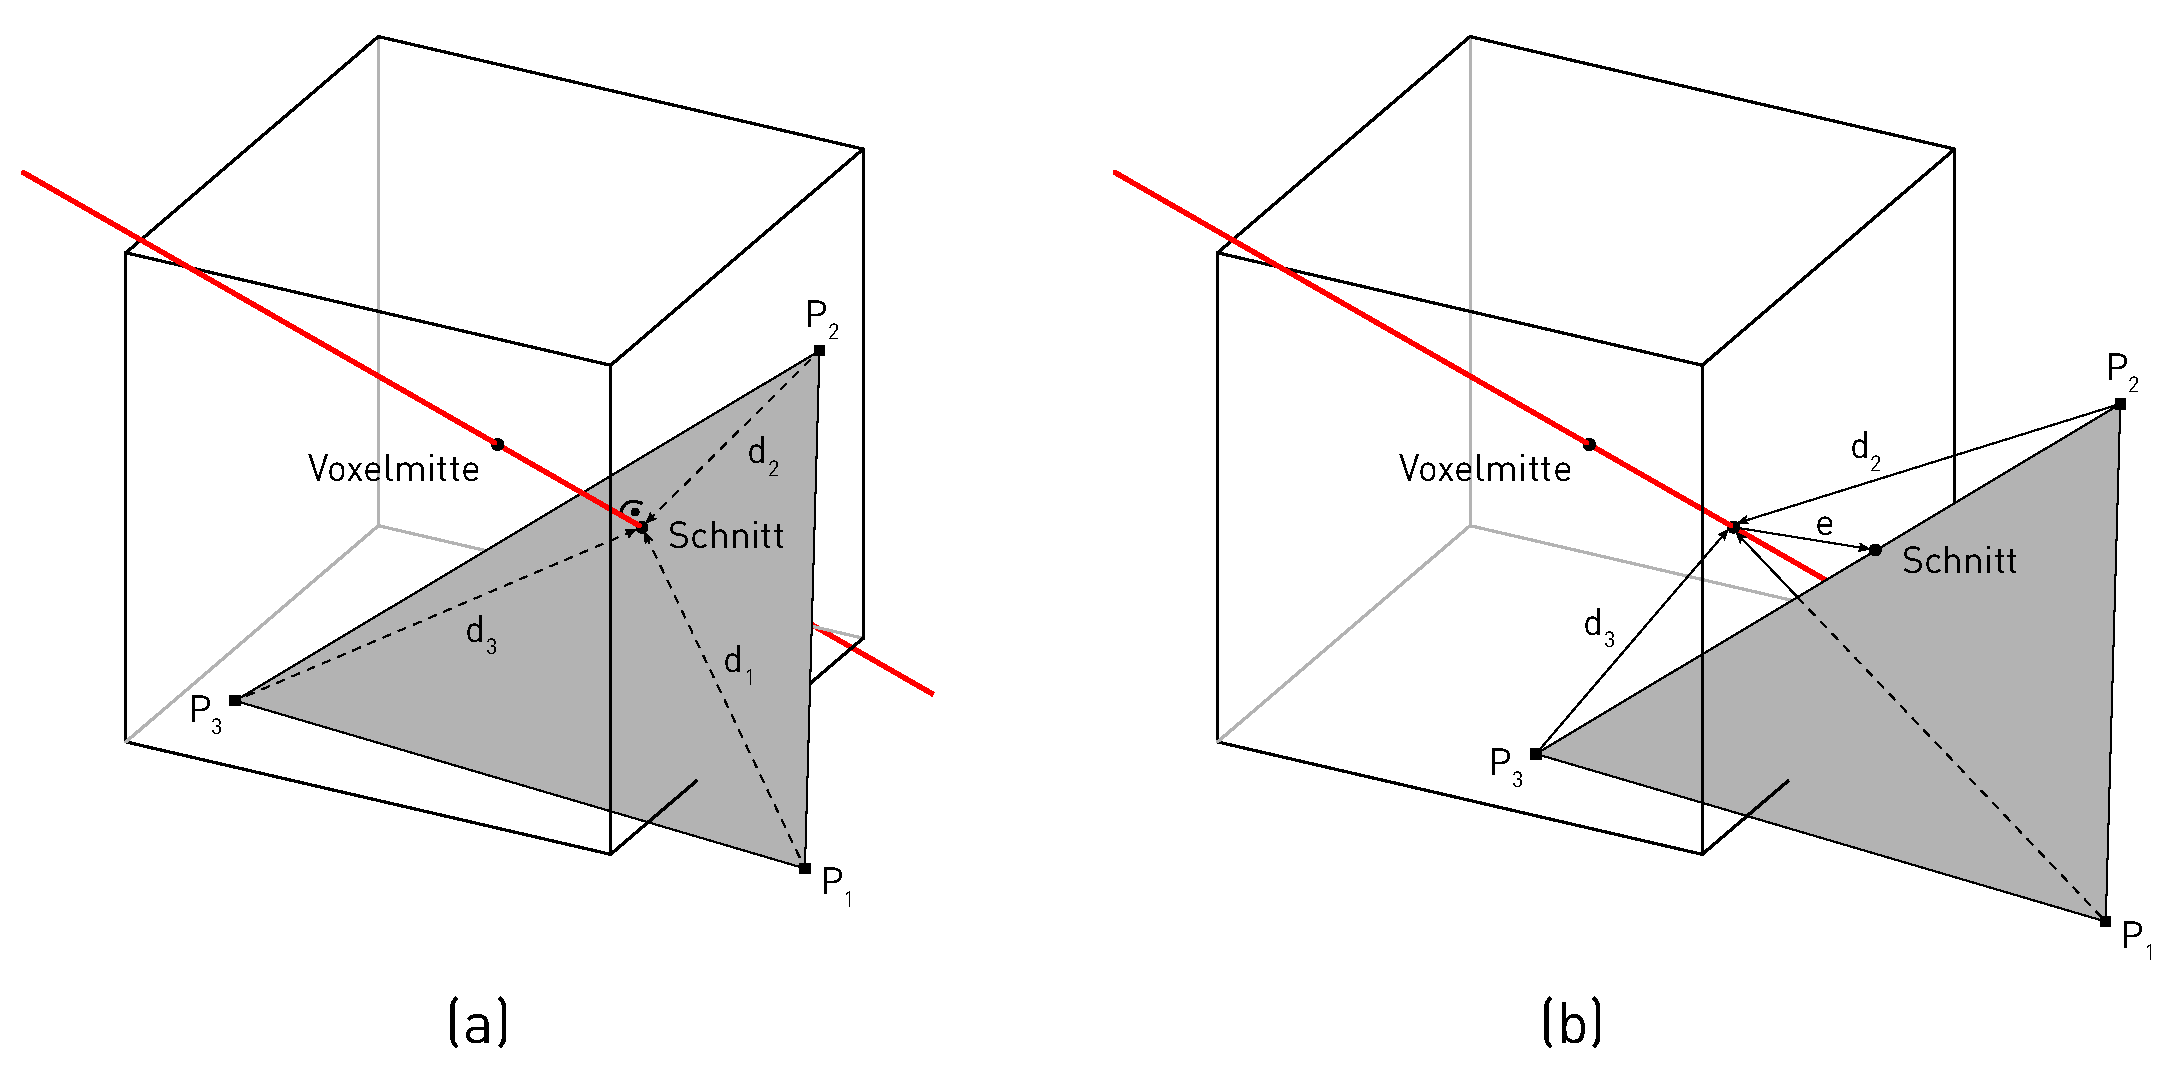
\includegraphics[width=0.85\textwidth]{figures/voxel_primitiv_schnitt.pdf}
  \caption{Ermittlung von UV-Koordinaten\label{voxel_primitiv_schnitt}}
\end{figure}
Durch die Wahl der Richtung ist gew�hrleistet, dass der Winkel zwischen Strahl und Dreicks\-fl�che maximal ist, so dass die Wahrscheinlichkeit eines Schnittes erh�ht wird. Trotzdem ist es m�glich, dass der Strahl das Dreieck verfehlt, da das Voxel das Dreieck bei\-spiels\-weise nur mit einer Ecke schneidet, die nicht zur Voxel-Mitte ausgerichtet ist (vgl. Abbildung \ref{voxel_primitiv_schnitt}b). Um trotzdem den Beitrag des Dreiecks zu den Voxel-Attributen ber�cksichtigen zu k�nnen,  wird in diesem Fall der Punkt auf dem Dreieck als Schnittpunkt angenommen, der den kleinsten Abstand zum Schnittpunkt mit der Dreiecksebene besitzt. Dieser Vorgang erzeugt ein Rauschen in den Daten das aber angesichts der geringen Gr��e der Blatt-Knoten und des daraus resultierenden geringen Fehlers nicht sichtbar ist. Mit Hilfe der ermittelten UV-Koordinaten k�nnen nun Attribute wie Farbe oder Richtung aus den Eckpunkten der Dreiecke interpoliert oder aus Texturen gelesen werden. Die erhaltenen Werte werden �ber alle am Voxel beteiligten Dreiecke gemittelt. Farb- und Richtungs\-werte werden auf 8 Bit pro Komponente quantisiert bevor sie in den Attributbuffer gespeichert werden.\\
\newpage
Wie in Abschnitt \ref{sec:erzeugung_treelet_struktur} beschrieben, werden die Attribute der inneren Knoten erst erzeugt, nachdem die Erstellung aller Treelets ab\-ge\-schlos\-sen ist. Durch die Verwendung eines FIFO-Kontainers im Build-Manager sind die Treelets so nummeriert, dass jedes Treelet einen niedrigeren Index besitzt als seine untergeordneten Treelets. Somit ist das Treelet mit dem h�chsten Index von keinem anderen Treelet f�r die Generierung seiner Attribute abh�ngig, da es schon in allen seinen Blatt-Knoten Attribute besitzt. Das Treelet mit dem Index $0$ ist dagegen f�r seine Attributgenerierung von allen anderen Treelets abh�ngig. F�r die Generierung der Attribute werden die Treelets daher in umgekehrter Reihenfolge ihrer Indizierung abgearbeitet. Abbildung \ref{attribute_generation} veranschaulicht die Reihenfolge anhand eines Beispiels (vgl. Abbildung \ref{fig:treelet_building}).
\begin{figure}[position=v]
  \centering
  \includegraphics[width=0.70\textwidth]{figures/attribute_generation.pdf}
  \caption{Reihenfolge der Erzeugung der Attributen innerer Knoten\label{attribute_generation}}
\end{figure}\\
Beginnend beim Treelet mit dem gr��ten Index wird jedes Treelet, vom Wurzelknoten an, der Tiefe nach, rekursiv durchlaufen bis die Blattknoten erreicht werden. Diese enthalten bereits Attribute\-informationen. Beim Aufsteigen aus der Rekursion werden die Attribute der jeweils vorhandenen Kindknoten gemittelt und im Attribut-Buffer abgelegt. Dazu werden die mit 8 Bit  aufgel�sten Attribut\-komponenten der Kindknoten zun�chst wieder in 32 Bit Flie�\-komma\-werte konvertiert, damit sich bei der Mittelung der Kindknotenattribute die Quantisierungsfehler nicht verst�rken. Nachdem auch f�r den Wurzelknoten ein Attribut vorhanden ist, wird dieses in den Attribut-Buffer des �bergeordneten Treelets f�r den entsprechenden Blattknoten abgelegt. Durch die Reihenfolge der Indizierung ist f�r jedes Treelet sichergestellt, dass f�r alle Blatt\-knoten Attributinformationen vorhanden sind wenn sie zur Generierung der Attribute der inneren Knoten ben�tigt werden.




\newpage

\section{Echtzeitf�higes Sparse Voxel Octree Streaming}\label{sec:echtzeitfaehiges_svo_raycasting}


% ////////////////////////////////////////////


\subsection{�berblick der Verarbeitungsschritte}
Im Folgenden soll der Ablauf der dynamischen Ver�nderung der SVO-Struktur im Incore-Buffer abh�ngig von der Kameraposition erl�utert werden. In den nachfolgenden Kapiteln wird auf die einzelnen Schritte genauer eingegangen. Die Abfolge der beteiligten Teilprozesse k�nnen in Abbildung \ref{ablauf_farbe} nachvollzogen werden. \\
Der Incore-Buffer wird zun�chst mit dem Wurzel-Treelet im ersten Slot initialisiert. Die adaptive Anpassung der Baumstruktur wird in vier Schritten realisiert: Zun�chst wird der Octree aus der Sicht der Kamera in den Analyse-Buffer gerendert (\textit{Analyse-Pass}). Nach diesem Schritt enth�lt dieser Buffer f�r jeden Strahl unter anderem die Position des getroffenen Knotens im Incore-Buffer und einen Fehler\-wert. Der Fehler\-wert ergibt sich dabei aus dem Unterschied der Fl�che der Projektion des getroffenen Voxels zur Gr��e eines Pixels des verwendeten Bild-Buffers (vgl. Lacoste et al. \cite{Lacoste_2007}). War der getroffene Knoten ein Blatt, zu dessen Verfeinerung ein Treelet vorhanden ist, wird zus�tzlich noch dessen Index gespeichert.

\begin{figure}[position=h]
  \centering
  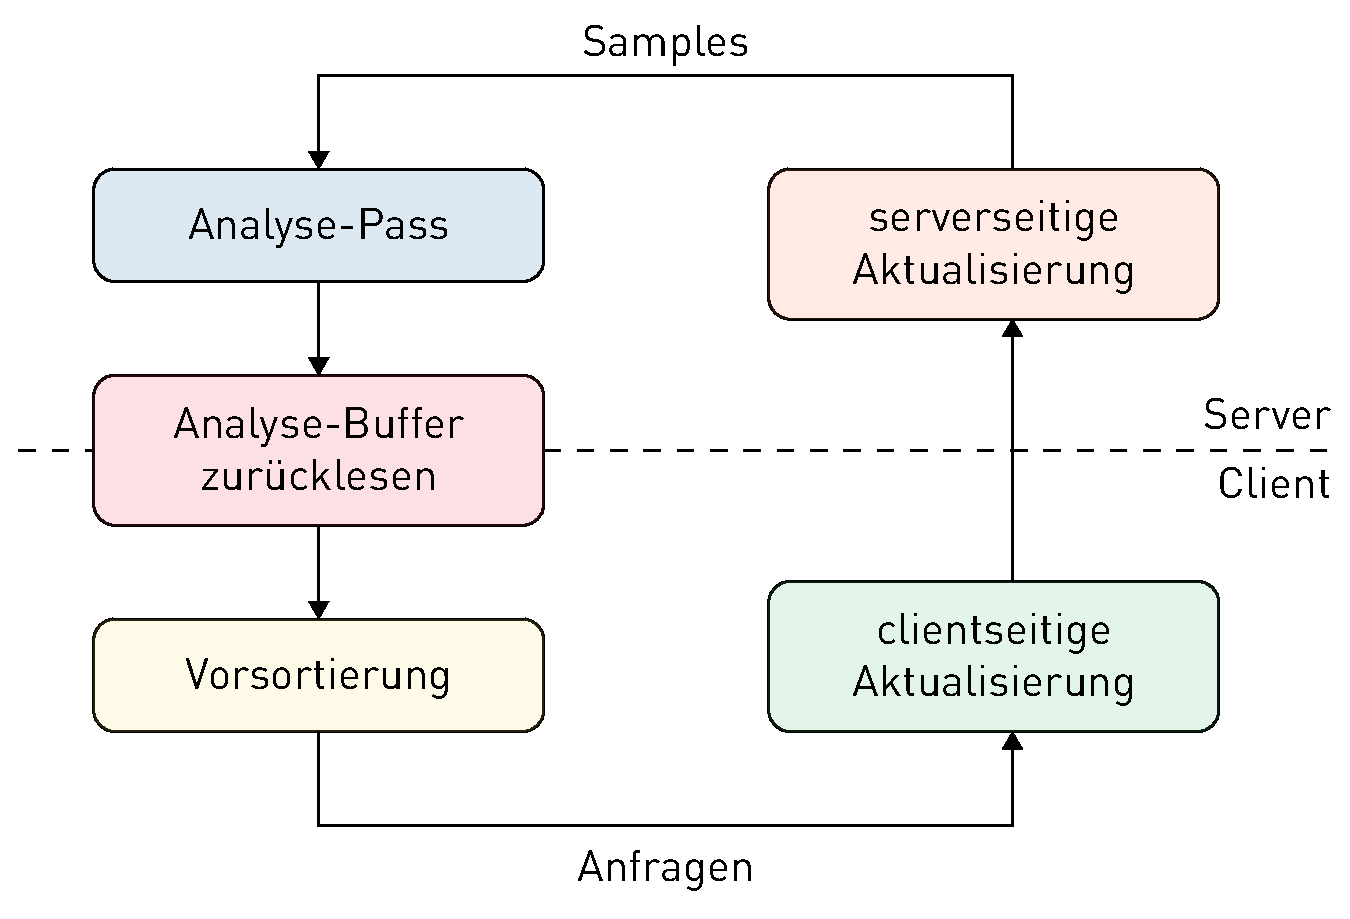
\includegraphics[width=0.68\textwidth]{figures/ablauf_farbe.pdf}
  \caption{Ablauf der Verarbeitsschritte des Out-of-Core-Systems\label{ablauf_farbe}}
\end{figure}

Nach der �bertragung des Feedback-Buffers in den Hauptspeicher werden dessen Eintr�ge in zwei Container einsortiert (\textit{Vorsortierung}). Der eine enth�lt die Treelet-Indices aller Knoten die sichtbar sind sowie die Treelet-Indices ihrer �bergeordneten Treelets bis zum Wurzel-Treelet. Der andere Container ent\-h�lt Anfragen nach Verfeinerung in Form der Indices der anzuh�ngenden Treelets. Die Fehler\-werte bleiben dabei in beiden Containern erhalten. Beide Container werden dem Speichermanagement �bergeben (\textit{clientseitige Aktualisierung}). Dort werden zun�chst die Sichtbarkeitsinformationen aller im letzten Zyklus sichtbarer Treelets aktualisiert. Danach werden die neu anzuh�ngenden Treelets in den clientseitigen Incore-Buffer eingepflegt. Stehen im Incore-Buffer keine freien Slots mehr zur Verf�gung werden nicht sichtbare Treelets entfernt. Slots mit ver�ndertem Inhalt werden markiert. Anschlie�end werden die ver�nderten Bereiche des Incore-Buffers an den Server �bertragen und stehen nun dem Renderer f�r den n�chsten Zyklus zur Verf�gung (\textit{serverseitige Aktualisierung}).



% ////////////////////////////////////////////



\subsection{Analyse-Pass}\label{sec:streaming_analyse_pass}

Um die Last, die durch diesen zus�tzlichen Render-Pass entsteht, m�glichst gering zu halten ist die Gr��e des zur Analyse verwendeten Buffer wesentlich kleiner als die des f�r die Bildgenerierung verwendeten Frame-Buffers. Um Artefakt\-bildung zu vermindern werden die Strahlen bei jedem Analyseschritt durch Zufalls\-werte parallel zur Sicht-Ebene verschoben. Die Verschiebung ist dabei so gew�hlt, dass �ber die Zeit im Bereich von $n*n$ Texeln des Bild-Buffers gesampelt wird, wobei $n$ das Verh�ltnis der Gr��en von Frame-Buffer und Analyse-Buffer ist.
In Tests war es m�glich, den Analyse-Buffer bis auf ein Achtel der Gr��e des Bild-Buffers zu verkleinern ohne dass es durch Aliasing zu Artefaktbildung kam oder zu wenig Daten f�r die nachfolgende dynamische Anpassung des Octrees zur Verf�gung standen.\\
Das F�llen des Analyse-Buffers erfolgt analog zum bilderzeugenden Raycasting mit OpenCL auf dem, im Incore-Buffer vorhanden Octree. Nach der Traversierung des Octrees liegt f�r jeden Strahl eines der folgenden drei Ergebnisse vor:  
\begin{enumerate}
  \item der Strahl trifft keinen Knoten 
  \item der Strahl trifft einen inneren Knoten
  \item der Strahl trifft einen Blattknoten
\end{enumerate}
Im ersten Fall wird nichts zur�ckgegeben. Im zweiten Fall wird nur die Position des Voxels im Incore-Buffer und die L�nge des Strahles zur�ckgegeben. Im dritten Fall wird zus�tzlich der Verweis auf ein eventuell anh�ngbares Treelet zur�ckgegeben. Ausserdem wird die Differenz zwischen vorgefundener Voxelgr��e und der f�r die L�nge des Strahles idealen Voxelgr��e als Fehler\-wert gespeichert. Abbildung \ref{oversampling_aliasing} zeigt die Bildung des Fehler\-wertes. Listing 4.2 zeigt den Aufbau eines Analyse-Buffer-Elements.

\begin{figure}[position=h]
  \centering
  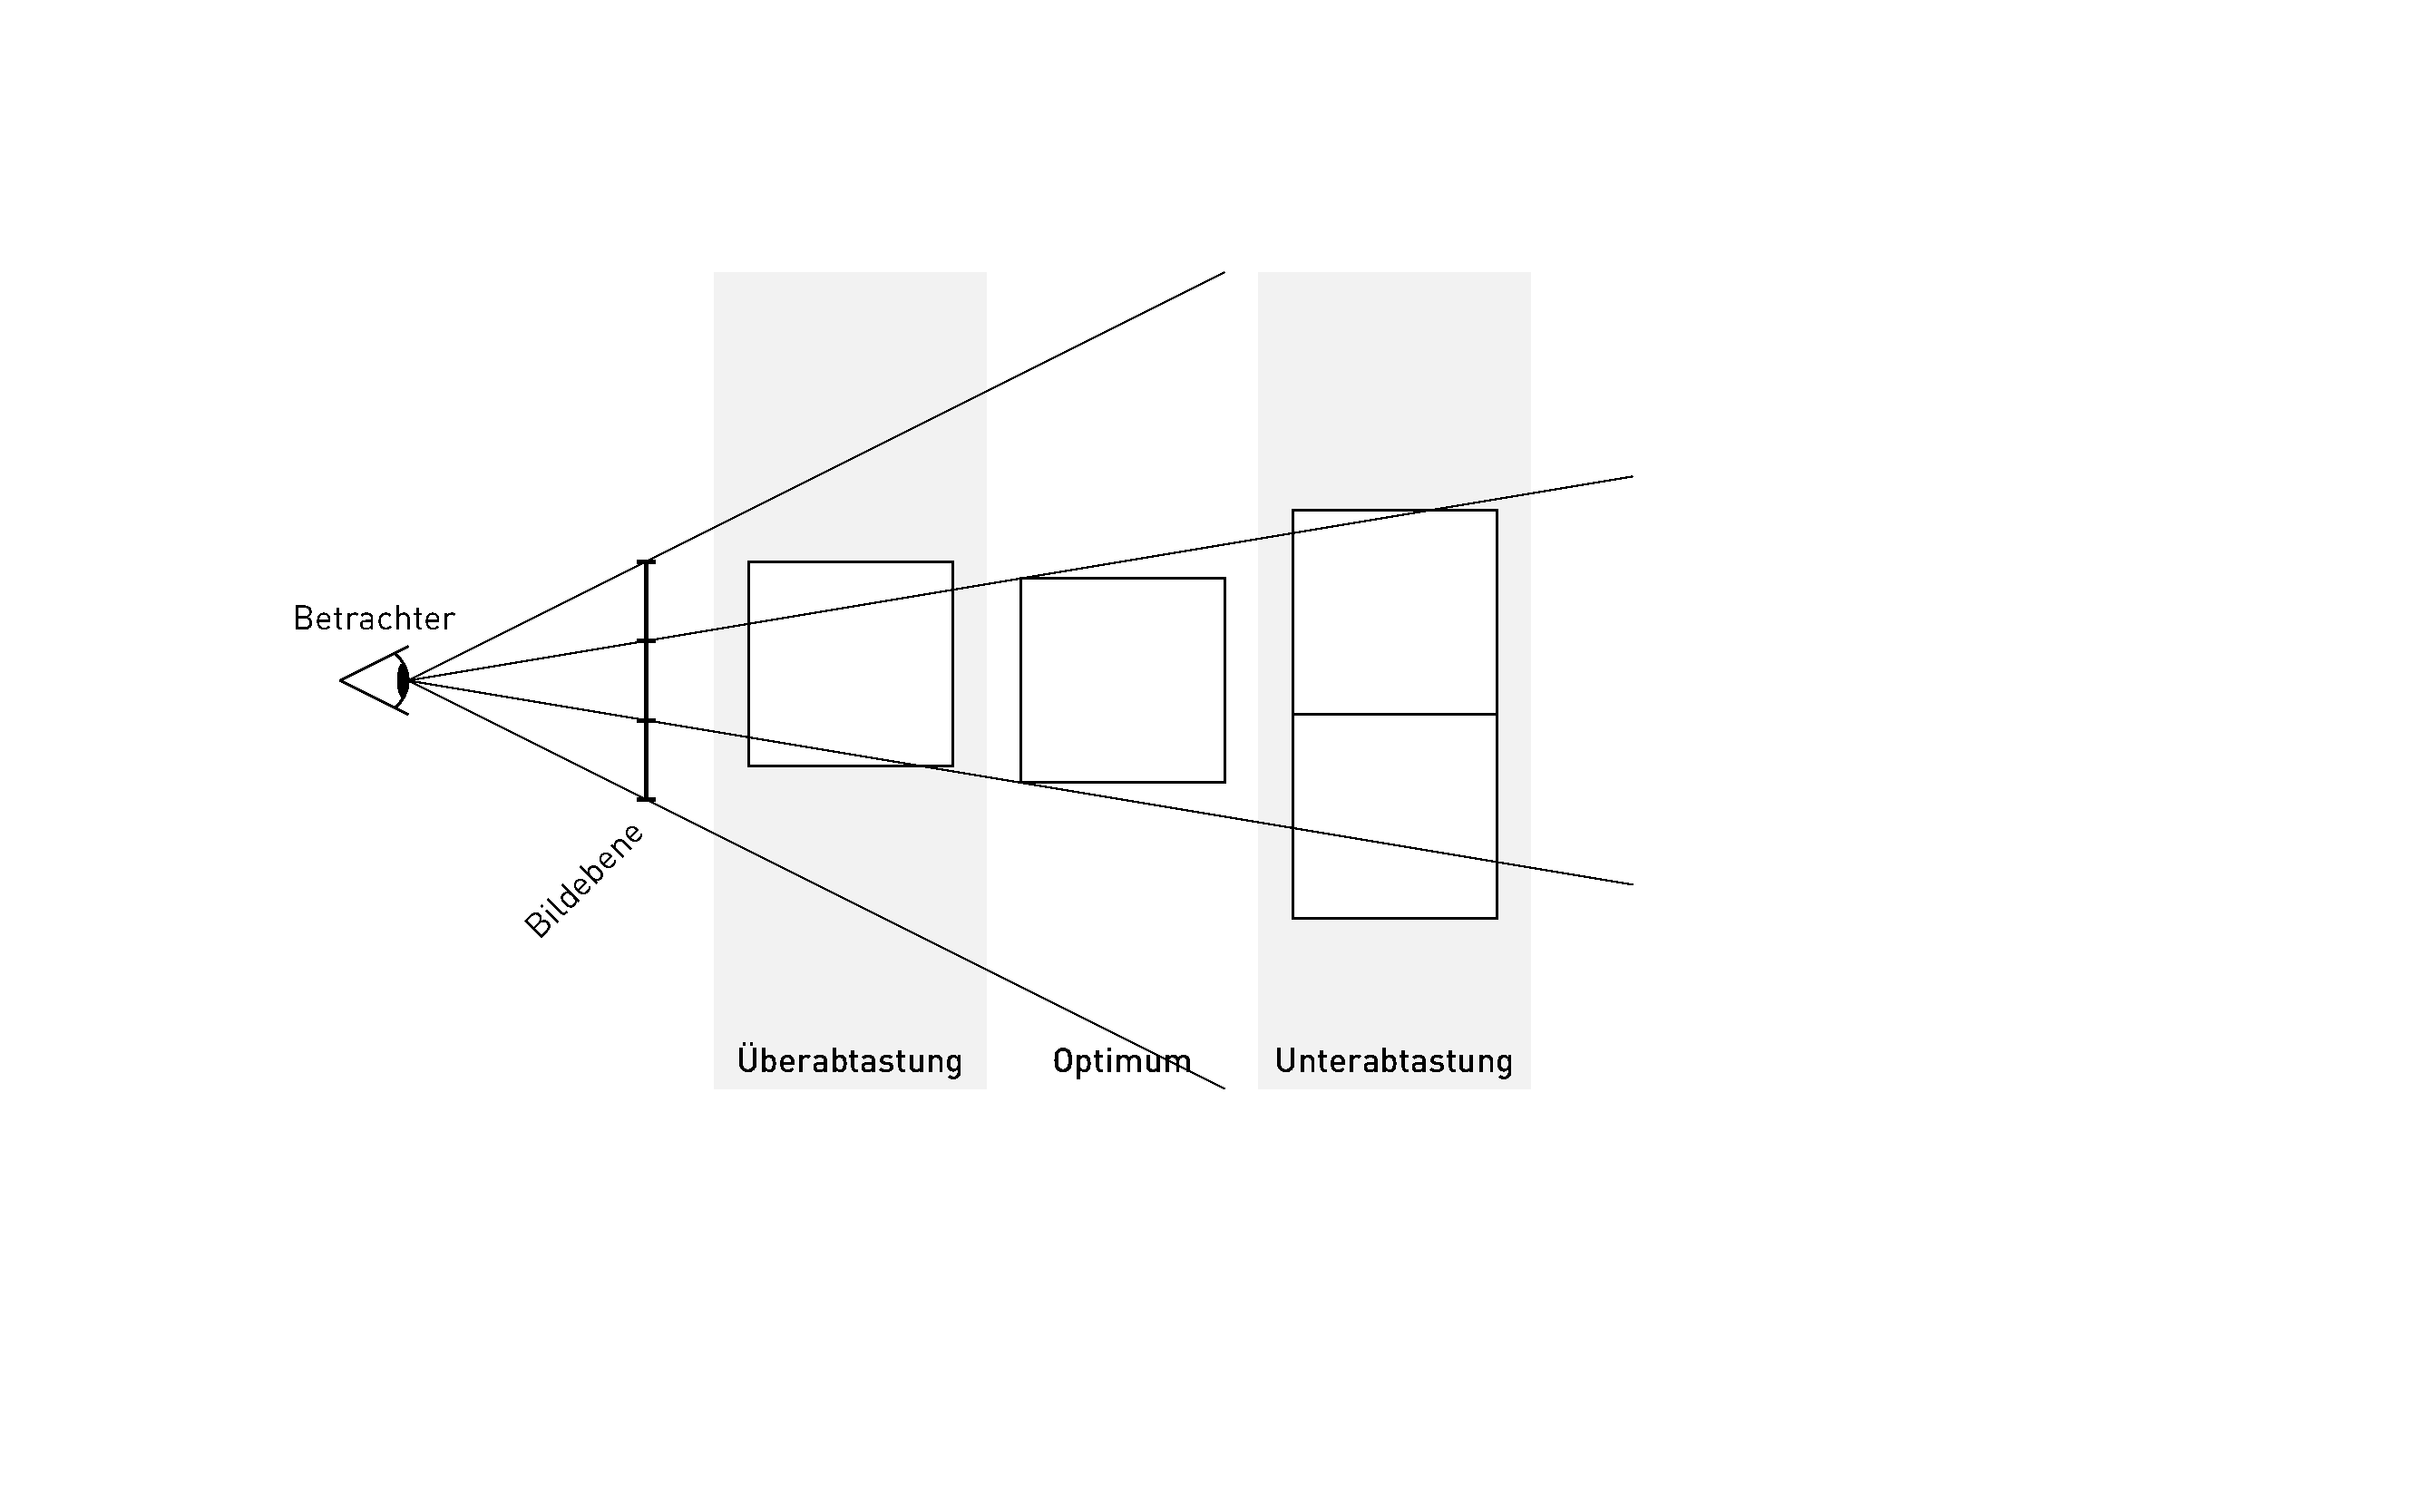
\includegraphics[width=0.75\textwidth]{figures/oversampling_aliasing.pdf}
  \caption{Fehlerma� bei der �berabtastung der Voxel\label{oversampling_aliasing}}
\end{figure}

\newpage

\begin{lstlisting}[caption=Struktur eines Analyse-Buffer-Elements]{lst:structFeedBackDataElement}
  struct FeedBackDataElement
  {
    // Knoten-Index im Incore-Buffer in dem der Strahl terminierte
    int   _nodeId;
    // Unterschied zwischen geforderter und erreichter Voxelgr��e
    float _error;
    // Treelet-Index, falls der Strahl in einem Blatt terminierte
    int   _subTreeletGid;
    // Entfernung von Kamera und Knoten (nicht notwendig f�r den beschriebenen Ablauf)
    float _tmin;
  };
\end{lstlisting}


\subsection{Vorsortierung}\label{sec:streaming_vorsortierung}

Nach der �bertragung des Analyse-Buffers vom Server in den Hauptspeicher werden dessen Elemente ausgewertet. Dabei werden zwei Container mit unterschiedlichen Sicht\-informationen gef�llt. Im ersten Container werden Indices von Treelets notiert, die bereits im Incore-Buffer vorhanden sind. Der zweite Container enth�lt nur Anfragen nach neuen Treelets. Beide Container sind nach dem Fehler\-wert der Eintr�ge absteigend sortiert wobei jeder Treelet-Index �ber beide Container hinweg unique ist.\\
Im oben beschriebenen Fall 1 (der Strahl trifft keinen Knoten) liegt keine Sichtbarkeitsinformation vor, weshalb solche Eintr�ge �bersprungen werden. Im Fall 2 (der Strahl trifft einen inneren Knoten) wird �ber die erhaltene Position des Knotens im Incore-Buffer und �ber die Gr��e eines Treelets auf den Slot des zugeh�rigen Treelets und damit auch auf das entsprechenden Treelet selbst geschlossen. Durch die in den Treelets gespeicherten Eltern-Information werden zus�tzlich alle �bergeordneten Treelets als sichtbar notiert. Tritt bei der Notation ein Treelet mehrfach auf, wird jeweils der gr��te Fehler �bernommen.\\
Im Fall 3 (der Strahl trifft einen Blattknoten) wird f�r den Blattknotenindex wie im Fall 2 vorgegangen. Zus�tzlich wird der Treelet-Index des anh�ngbaren Treelets im entsprechenden Container gespeichert. Tritt ein Treelet-Index mehrfach auf wird auch hier nur ein Eintrag mit dem gr��ten Fehler gespeichert.\\
Damit ist die Trennung der Sichtbarkeitsinformation abgeschlossen. An diesem Punkt kann die Menge der Anfragen noch auf einen Maximalwert begrenzt werden um die Last f�r die folgenden Schritte zu begrenzen, was die Verfeinerung des Octrees verlangsamt. Die absteigende Sortierung der Anfragen nach ihrem Fehler bei der Darstellung des Voxels sorgt daf�r, dass bei einer Begrenzung der Menge der Anfragen immer diejenigen weiterverarbeitet werden, die den gr��ten Beitrag zur Bildqualit�t liefern. Anschlie�end werden beide Container der Speicherverwaltung f�r die clientseitige Aktualisierung �bergeben.


% ////////////////////////////////////////////

\newpage
\subsection{Clientseitige Aktualisierung}

Nun sollen die ermittelten Sichtbarkeitsinformationen eingepflegt und Anfragen nach neuen Treelets durch Ver�nderungen der Octree-Struktur umgesetzt werden. Nach diesem Schritt �ndert sich auch die Belegung des clientseitigen Incore-Buffers.\\
Die Pflege der Sichtbarkeitsinformationen der bereits im Incore-Buffer befindlichen Treelets ist einfach: Zun�chst wird die Sichtbarkeit jedes Slots, d.h. jedes im Incore-Buffer befindlichen Treelets dekrementiert. Dann werden diejenigen Treelets aktualisiert, die beim let\-zten Analyse-Pass sichtbar waren. Dabei wird die Sichtbarkeit auf einen vorher festgelegten Maximalwert gesetzt der dem Gr��enverh�ltnis von Render-Buffer und Analyse-Buffer entspricht. %Da die Anzahl der berechneten Samples im Analyse-Buffer bei einem Gr��enverh�ltnis von $1/8$ nur einem $1/64$ der berechneten Pixel im Framebuffer entspricht w�hre anzunehemen das die miximale Sichtbarkeitswert h�her sein m�sste. 

\subsubsection{Einf�gen eines Treelets}
F�r das Einf�gen eines Treelets aus dem in der Vorsortierung erstellten Container wird zun�chst ein freier Slot innerhalb des Incore-Buffers ben�tigt. Ist dieser vorhanden, kann das Treelet an die ensprechende Stelle im Incore-Buffer kopiert werden. Der Slot-Index wird im Treelet-Objekt gespeichert und zur Aktualisierung des serverseitigen Incore-Buffers vorgemerkt. Die folgende Ver�nderung der Baumstruktur kann in Listing \ref{lst:insert_treelet} nachvollzogen werden. Aus dem Treelet werden folgende Werte gelesen:
\begin{enumerate}
  \item Der Treelet-Index des Eltern-Treelets,
  \item Der Knoten-Index des Blattknotens, an dem das Treelet angeh�ngt werden soll,
  \item Der Elternknoten-Index des Blattknotens,
  \item Die Position des Blattknotens in seinem Elternknoten.
\end{enumerate}
Damit wird nun die Position des entsprechenden Blatt\-knotens des Eltern-Treelets im Incore-Buffer ermittelt und durch den Wurzel\-knoten des anzuh�ngenden Treelets ersetzt. Durch diese Position muss dessen relativer Index zu seinem ersten Kindknoten angepasst werden. Der erste Kindknoten des neuen inneren Knotens findet sich immer an zweiter Position innerhalb des angeh�ngten Treelets im Incore-Buffer. Der Blattknoten wird damit zu einem inneren Knoten, was wiederum in seinem Elternknoten an der ent\-sprechen\-den Stelle in der Child-Mask vermerkt wird. In einem weiteren Container wird vermerkt, dass das Eltern-Treelet nun ein neues Kind-Treelet im Incore-Buffer besitzt. Abschlie�end wird der Slot-Index des Eltern-Treelets zur sp�teren serverseitigen Aktualisierung vorgemerkt.

\newpage

\lstinputlisting
    [caption={Einf�gen eines Treelets}
       \label{lst:insert_treelet},
       captionpos=t,language=C++]
 {listings/insert_treelet.cpp}
 

% ////////////////////////////////////////////


\subsubsection{Entfernen eines Treelets}
Ist f�r das Einf�gen eines Treelets kein Slot mehr verf�gbar, muss zun�chst ein Slot freigegeben werden, der ein nicht sichtbares Treelet enth�lt. Dazu wird der Baum der Treelets nebenl�ufig durchsucht und eine Menge von Kandidaten f�r das Entfernen vorgehalten. Aufgrund der Nebenl�ufigkeit dieser Suche ist nicht sichergestellt, dass ein Kandidat zum Zeitpunkt des Entfernens noch valide ist. Daher muss vor dem eigentlichen Entfernen des Slots zun�chst erneut die Sichtbarkeit �berpr�ft werden. Ausserdem ist es m�glich, dass zwar das entsprechende Treelet selbst nicht sichtbar ist, jedoch der entsprechende Blatt\-knoten des Eltern-Treelets, falls das Treelet entfernt werden w�rde. Dies geschieht nur an den R�ndern der Geometrie. Abbildung \ref{sichtstrahl_kanten_artefakt} stellt diesen Fall dar. Im Bild befindet sich ein geladenes Treelet hinter ei\-ner konvexen W�lbung der Geometrie und kann so nicht vom Analyse-Pass gesehen werden. Wird dieses Treelet jedoch entfernt, ragt der entstehende Blatt\-knoten des Eltern-Treelets (im Bild rot dargestellt) �ber die W�lbung hinaus. Im n�chsten Zyklus w�rde dieses Blatt wieder verfeinert werden wodurch es zu flackernden Artefakten an den Geometrie\-kanten kommt. Um diese Artefaktbildung zu verhindern wird die Sichtbarkeit des Eltern-Treelets ebenfalls �berpr�ft. Nur wenn auch das Eltern-Treelet nicht sichtbar ist, kann das Treelet sicher entfernt werden.\\
\begin{figure}[H]
  \centering
  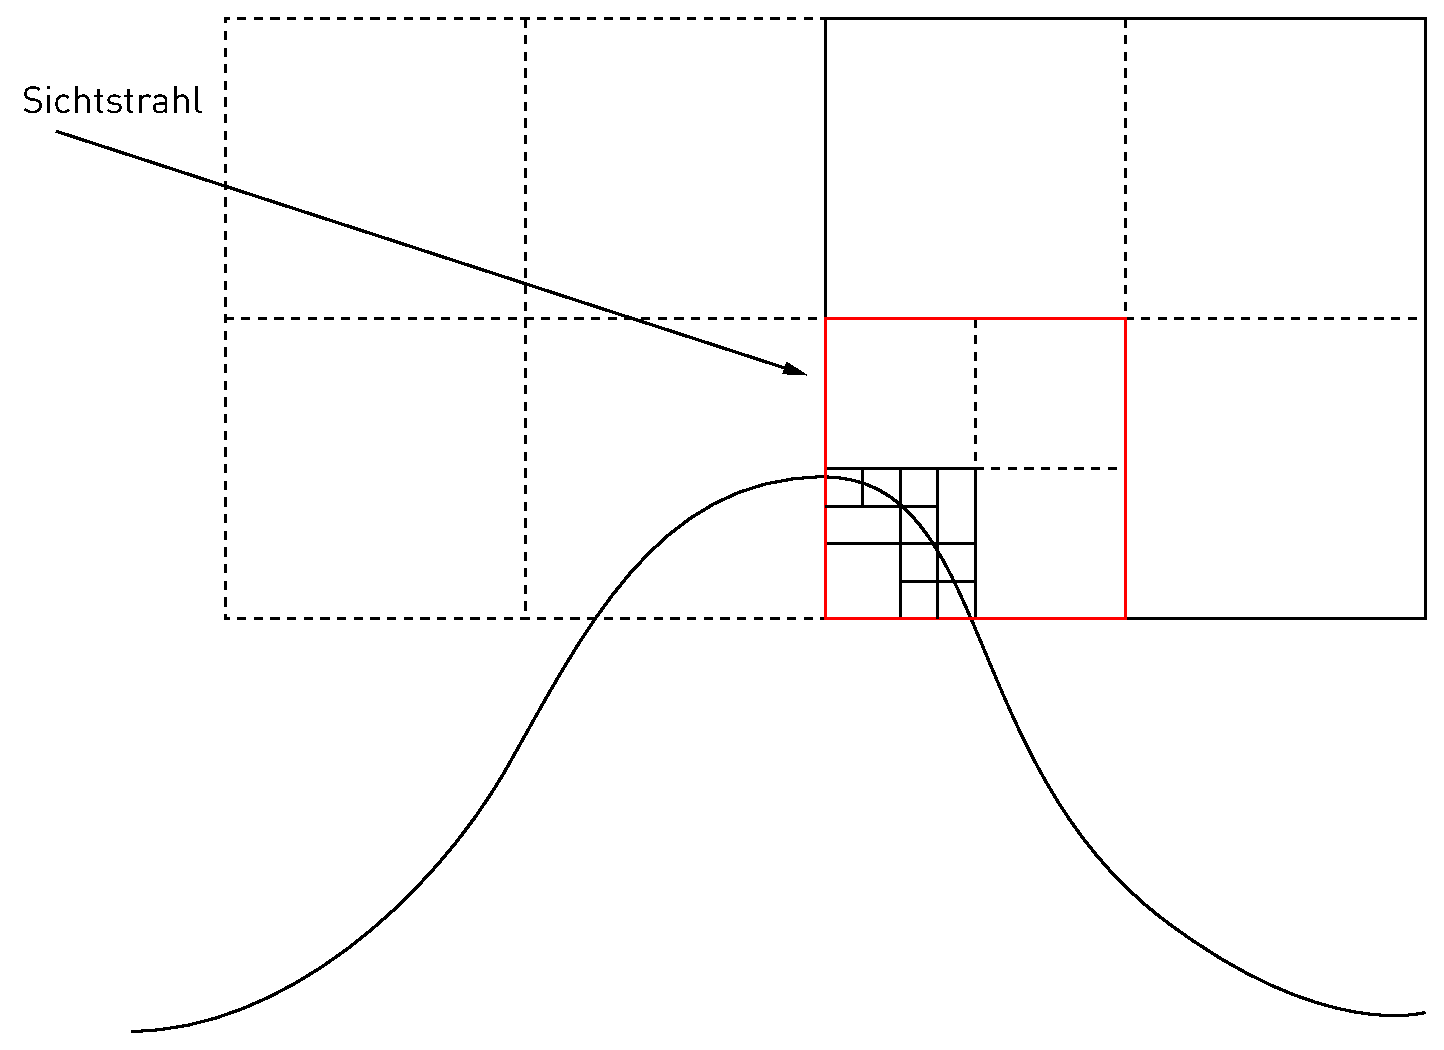
\includegraphics[width=0.75\textwidth]{figures/sichtstrahl_kanten_artefakt.pdf}
  \caption{Artefaktbildung and Objektkante\label{sichtstrahl_kanten_artefakt}}
\end{figure}
Alle Slots von im Incore-Buffer gespeicherten Treelets, die sich unterhalb des zu entfernenden Treelets befinden, k�nnen sofort freigegeben werden. Dazu wird f�r das Kan\-di\-daten-Treelet ermittelt, welche untergeordneten Treelets sich ebenfalls im Incore-Buffer befinden. So werden in einem g�nstigen Fall gleich mehrere Slots freigegeben.\\
Die Manipulation des Incore-Buffers zum Entfernen des Kan\-di\-daten-Treelets l�uft analog zum Einf�gen ab. Die folgenden Schritte k�nnen im Listing \ref{lst:remove_treelet} nachvollzogen werden. Wieder wird das Eltern-Treelet, die Position des entsprechenden Blattknotens und dessen Elternknotens ermittelt. Dann wird der Blatt\-knoten durch seine Repr�sentation aus dem Eltern-Treelet �berschrieben. Aus dem inneren Knoten wird so wieder ein Blattknoten mit einem Verweis auf ein anh�ngbares Treelet. Dies wird im Elternknoten des Blattknotens an der entsprechenden Stelle in der \textit{Child-Mask} markiert. Da sich damit das Eltern-Treelet im client\-seitigen Incore-Buffer ge�ndert hat muss dessen Slot zur server\-seitigen Aktualisierung vorgemerkt werden.
\newpage
\lstinputlisting
    [caption={Entfernen eines Treelets}
       \label{lst:remove_treelet},
       captionpos=t,language=C++]
 {listings/remove_treelet.cpp}

% ////////////////////////////////////////////

\newpage
\subsection{Serverseitige Aktualisierung}\label{sec:serverseitige_aktualisierung}

Die beim Einf�gen und Entfernen von Treelets markierten Slots werden in diesem Schritt auf den Server �bertragen. Dabei kann im einfachsten Fall jeder Slot innerhalb des Incore-Buffers einzeln �bertragen werden. Dies f�hrt jedoch zu vielen Einzel�bertragungen von geringer Gr��e. Dies ist sehr ung�nstig, da f�r jede Kopieroperation ein erheblicher Verwaltungsaufwand innerhalb der OpenCL-Implementation anf�llt. Handelt es sich beim verwendeten Server um eine GPU, m�ssen die Daten zus�tzlich �ber den PCI-Express-Bus �bertragen werden. Auch hier kann eine hohe �bertragungsrate nur durch m�glichst gro�e Pakete erreicht werden.\\
Um die Anzahl der Kopieraufrufe m�glichst gering zu halten werden deshalb nahe beieinander liegende Slots zusammengefasst und gemeinsam kopiert. Dazu werden die Indices der zu aktualisierenden Slots sortiert vorgehalten. Ausgehend vom ersten Slot-Index wird der zu kopierende Speicherbereich so lange bis zum n�chsten Slot erweitert bis das Verh�ltnis zwischen zu aktualisierenden Slots und unver�nderten Slots innerhalb dieses Bereiches unter einen festgelegten Grenzwert sinkt. Abbildung \ref{zusammenfassung_der_slots} zeigt das Ergebnis dieser Zusammenfassung f�r ein Verh�ltis von 50\% zwischen ver�nderten Slots und Gesamtzahl der Slots im zu kopierenden Bereich.
\begin{figure}[position=h]
  \centering
  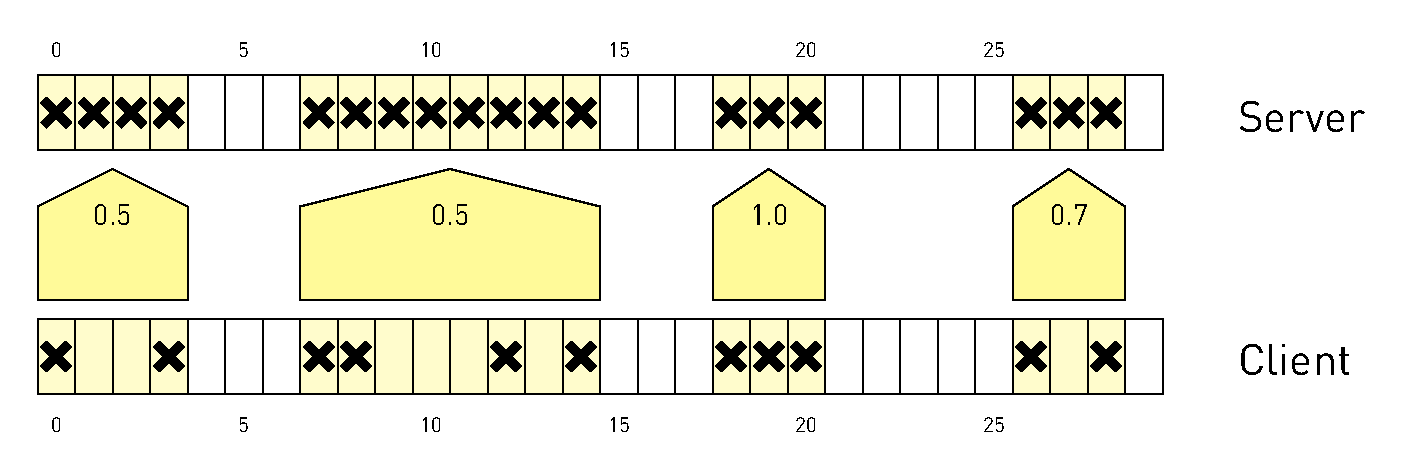
\includegraphics[width=0.85\textwidth]{figures/zusammenfassung_der_slots.pdf}
  \caption{Zusammenfassen von Slots zur �bertragung\label{zusammenfassung_der_slots}}
\end{figure}
Am effizientesten arbeitet dieser Ansatz, wenn der Incore-Buffer anfangs noch leer ist, da die Slots-Indices aufeinanderfolgend herausgegeben werden und die entsprechenden Speicherbereiche damit an einem St�ck auf den Server transferiert werden k�nnen. Das Zusammenfassen der Slots kann in einem Thread ausgelagert werden, damit sich der entstehende Zeitaufwand nicht auf die Bildrate auswirkt. Im Abschnitt \ref{sec:test_zusammenfassen_von_slots} (\nameref{sec:test_zusammenfassen_von_slots}) wird die Ermittlung eines geeigneten Wertes f�r das Verh�ltnis zwischen der Anzahl ver�nderter Slots und der Gesamtzahl von Slots im zu kopierenden Bereich untersucht.
\newpage

\newpage
\chapter{Ergebnisse und Diskussion}\label{se:ergebnisse_diskusionen}



% /////////////////////////////////////////////////////////



\section{�berblick}
Abbildung \ref{lucy_s4_D13_timeseries} gibt einen allgemeinen Eindruck �ber die Laufzeiten der einzelnen Teilschritte, die in Abschnitt \ref{sec:echtzeitfaehiges_svo_raycasting} \textit{\nameref{sec:echtzeitfaehiges_svo_raycasting}} beschrieben wurden sowie �ber die Anzahl verarbeiteter Treelets. Die Werte wurden in Abst�nden von 200 ms aufgezeichnet.
\begin{figure}[H]
  \centering
  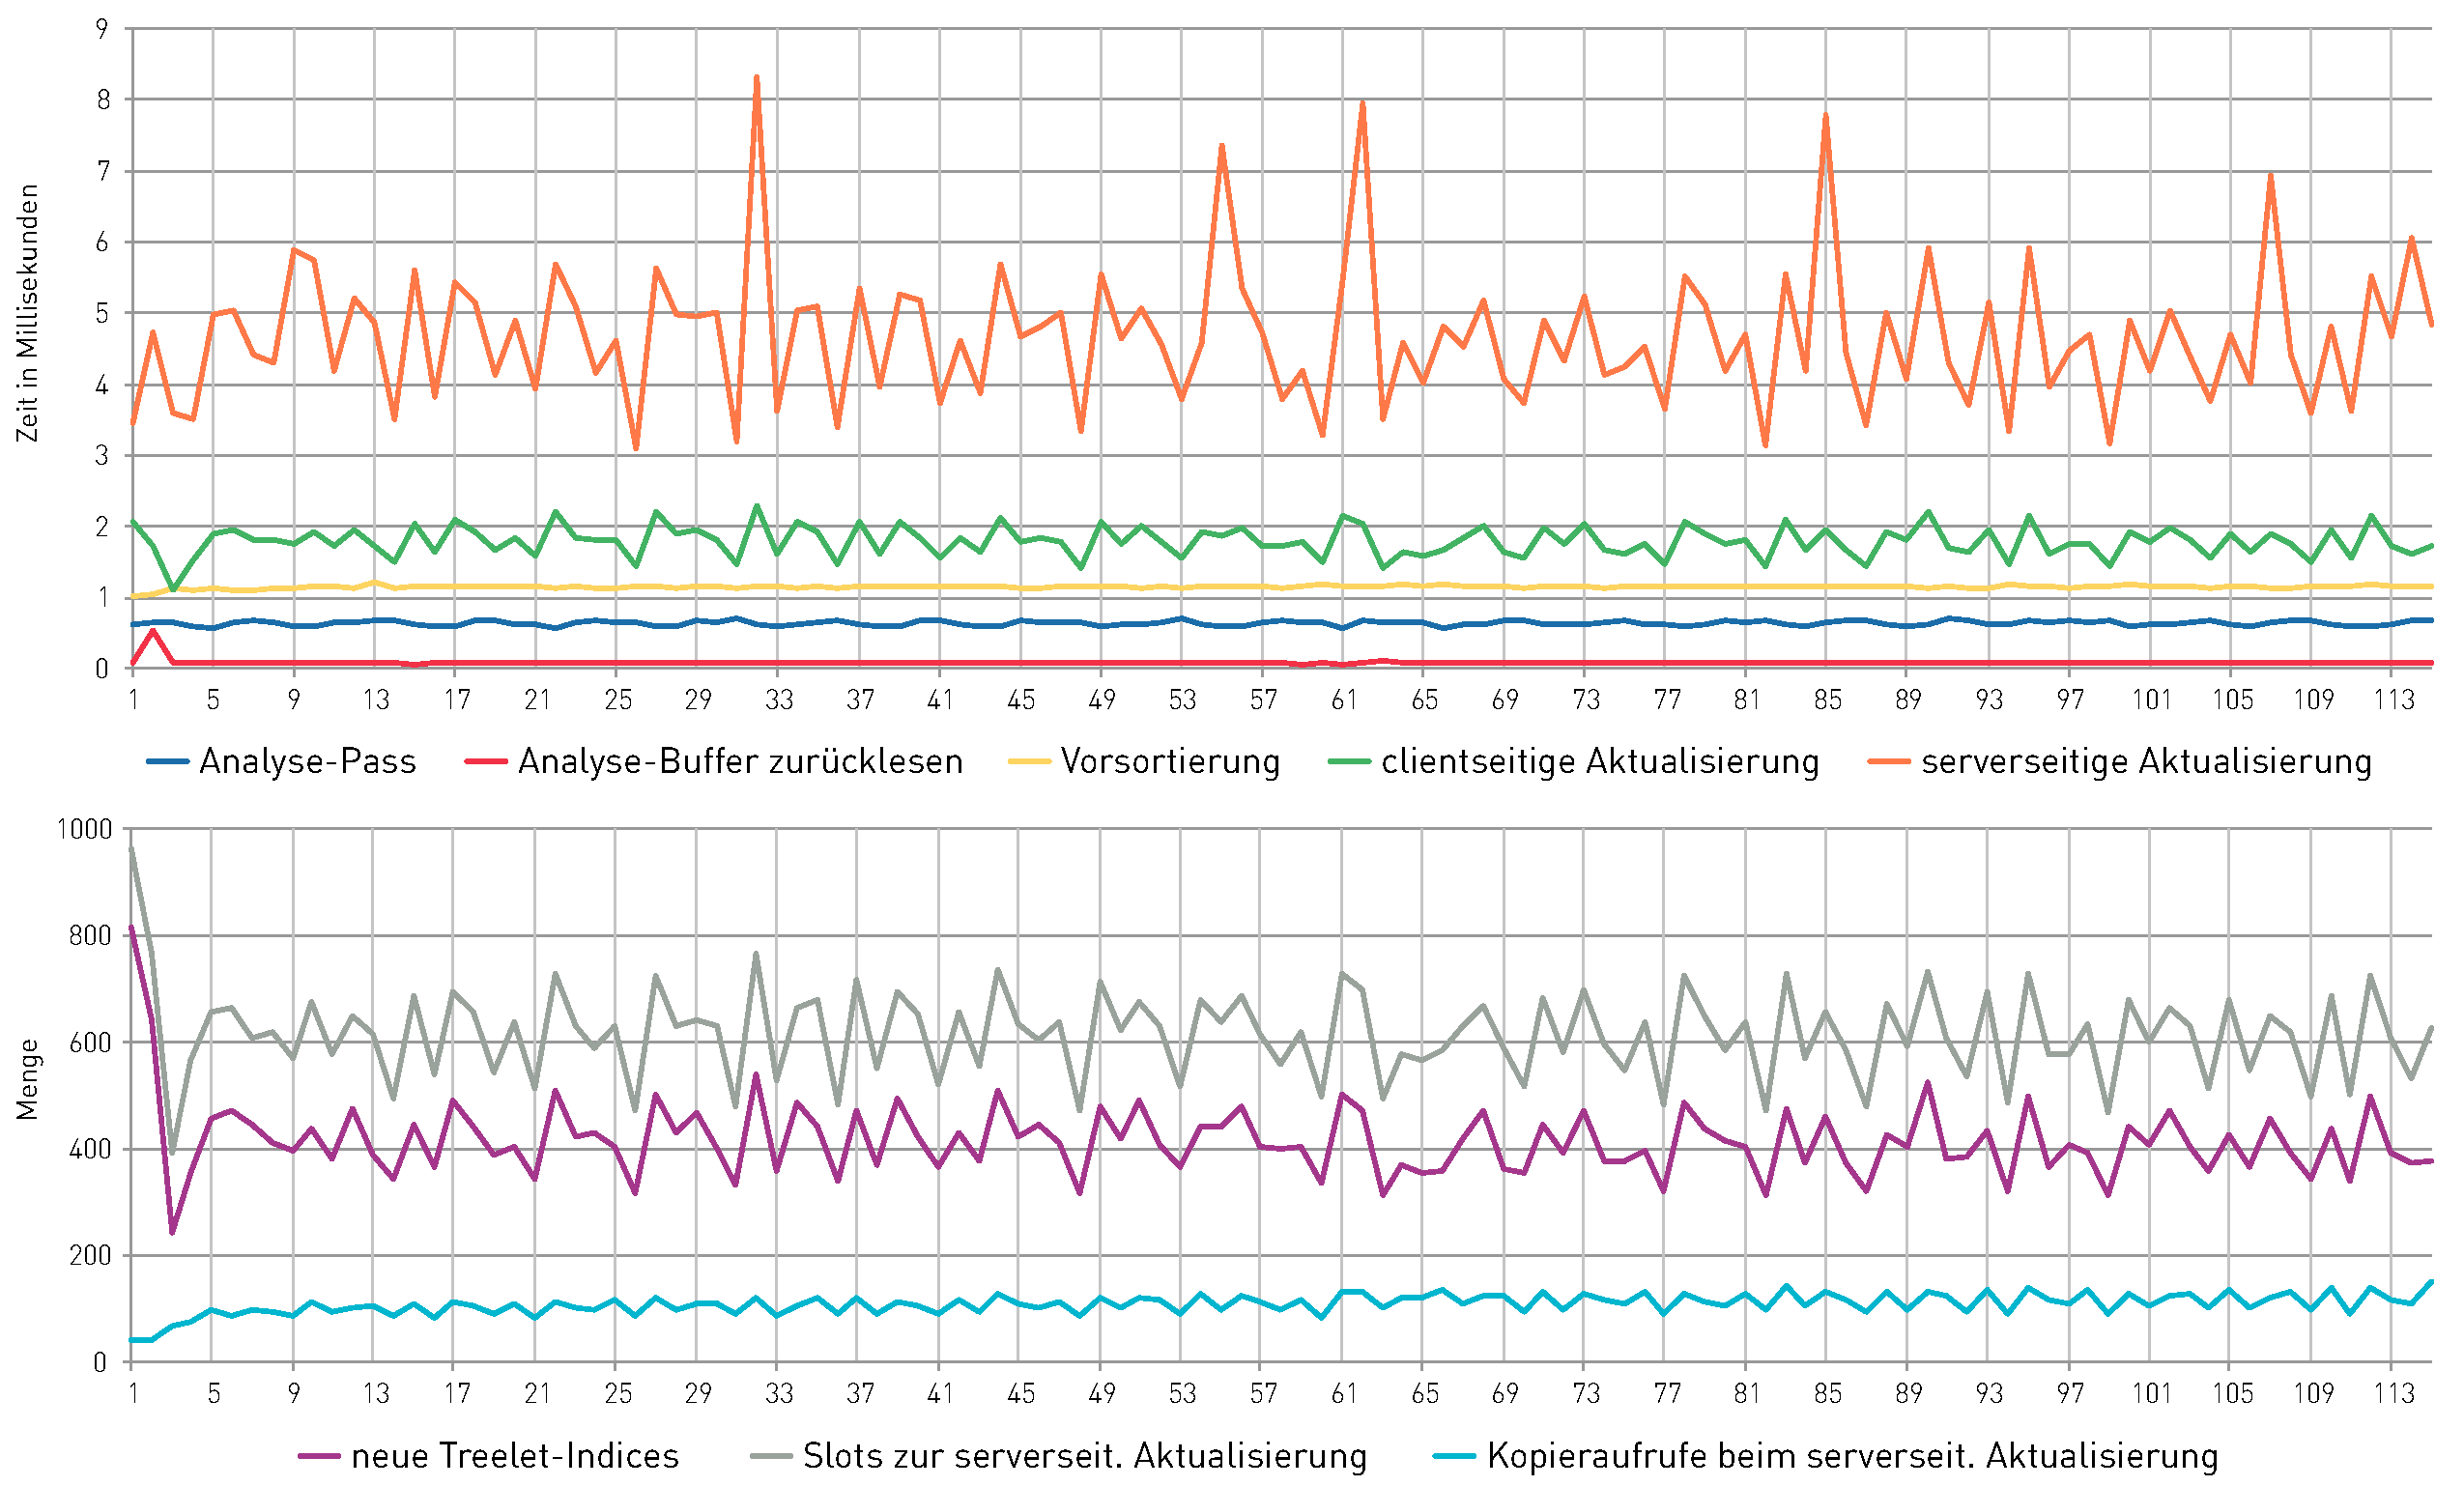
\includegraphics[width=1.0\textwidth]{figures/lucy_s4_D13_timeseries.pdf}
  \caption{Systemzeiten und zu verarbeitende Treelets\label{lucy_s4_D13_timeseries}}
\end{figure}
Im oberen Teil der Abbildung finden sich die Zeiten f�r das Bef�llen und die �bertragung des Analyse-Buffers sowie die Vorsortierung in Sichtinformationen f�r neue und bereits geladene Treelets. Ausserdem sind die ben�tigten Zeiten f�r die Pflege des clientseitigen und serverseitigen Incore-Buffers dargestellt. Im unteren Graphen sind die Mengen der von der Analyse des Baumes erzeugten Anfragen nach neuen Treelets, die Anzahl der daraufhin ge�nderten Slots und die Anzahl der ben�tigten Kopieraufrufe dargestellt.\\
Um die Eigenschaften und Leistungsf�higkeit des Systems zu analysieren wurden im Zuge dieser Arbeit drei Tests durchgef�hrt. Der erste Test untersucht den Einfluss der Treelet-Gr��e auf das Verhalten des Out-of-Core-Systems. Der zweite Test untersucht das Verfahren zur Minimierung der Kopieraufrufe bei der serverseitigen Aktualisierung (vgl. Abschnitt \ref{sec:serverseitige_aktualisierung} \textit{\nameref{sec:serverseitige_aktualisierung}} ). Ein dritter Test soll die Reaktionsf�higkeit des Systems w�hrend der Benutzung untersuchen.\\
Als Testsystem stand ein aktuelles GNU/Linux-System mit Intel Core i7-2600 (3.4 GHz) und 32 GB Arbeitsspeicher zu Verf�gung. Eine Nvidia GForce 580 GTX mit 1.5 GB Ram war �ber PCI-Express 2 angebunden. 


% /////////////////////////////////////////////////////////


\section{Verwendete Testmodelle}
 
Als Testdaten wurden drei Dreiecksmodelle mit Hilfe des in Kapitel \ref{sec:erzeugung_treelet_struktur} (\textit{\nameref{sec:erzeugung_treelet_struktur}}) beschriebenen Systems in Sparse Voxel Octrees �berf�hrt. Aus jedem Modell wurden jeweils zwei SVO-Strukturen erstellt. Beide Varianten haben die gleiche minimale Tiefe von 13 f�r alle Blattknoten, unterscheiden sich aber in der Treelet-Gr��e. Diese betr�gt jeweils 1 kB und 4 kB. Tabelle \ref{tab:verwendete_modelle} zeigt die Anzahl der Dreiecke der verwendeten Ausgangsmodelle und die Anzahl von Treelets und Voxeln der resultierenden Octrees. 
F�r alle Octrees wurden Attribut-Buffer mit Farb- und Normalenwerten erstellt die mit 16 Byte/Voxel aufgel�st sind.\\
Das Modell \textit{david face} stellt eine Besonderheit dar. Durch die feste Segmentgr��e ist die Darstellung mit 4 kB-gro�en Treelets unverh�ltnism�ssig gro� geworden.\\
Die SVO-Repr�sentationen der Dreiecksmodelle sind in den Darstellungen mit 4 kB und 1 kB gro�en Treelets unterschiedlich gro�. Dies ist auf die feste Segmentgr��e zur�ckzuf�hren. Sie bleiben jedoch trotzdem vergleichbar, da durch die Wirkungsweise des Systems nur Teile der Strukturen verarbeitet werden die f�r die Darstellung ben�tigt werden.


\begin{table}[position=h]
\changefont{ptm}{m}{n}
\normalsize
\centering
\begin{tabular}{ l  r  r  c  r r r}
\toprule
\textbf{Name} & \textbf{Dreiecke} & \textbf{Dateigr��e} & \textbf{Treelet-Gr��e} & \textbf{Treelets} & \textbf{Voxel} & \textbf{Dateigr��e} \\
\midrule
  david face        & 52.5 Mio & 1.47 GB & 1kb & 743.277 &  95.139.456 & 1.4 GB \\

                    &          &         & 4kb & 484.297 & 247.960.064 & 3.7 GB \\
\midrule
  Lucy              & 28.0 Mio & 757 MB & 1kb & 588.032  & 75.268.096 & 1.2 GB \\
                    &          &        & 4kb & 131.072  & 67.108.864 & 1.0 GB \\
\midrule
  xyzrgb statuette  & 10.0 Mio & 270 MB & 1kb & 781.302 & 100.006.656 & 1.5 GB \\
                    &          &        & 4kb & 246.434 & 126.174.208 & 1.9 GB \\ 
\bottomrule 
\end{tabular}\\
%\vspace{0.2cm}
%\hrule height 1pt width 1.0\hsize
\caption{Verwendete Modelle}\label{tab:verwendete_modelle}
\end{table}

% /////////////////////////////////////////////////////////////

\newpage

\section{Einfluss der Segmentgr��e auf das Systemverhalten}\label{sec:test_einfluss_groesse}

\subsection{Versuchsaufbau}
Bei diesem Test soll der Einfluss der Speichergr��e der Treelets auf das Laufverhalten des Systems untersucht werden. Dazu wurden f�r alle sechs Octrees die Werte, wie sie in Abbildung \ref{lucy_s4_D13_timeseries} dargestellt sind, aufgenommen. Die Aufnahme\-zeit betrug in allen Durchl�ufen 30 Sekunden. In Intervallen von 200 ms wurde jeweils der Mittelwert aller in dieser Zeit erfolgten Programmzyklen notiert.\\
Um das System zu belasten und eine anhaltende Ver�nderung des Incore-Buffers anzuregen, wurden alle Modelle vor der Kamera mit $1/3$ Hz um die Hochachse rotiert. Mit der Bewegung sollte gew�hrleistet werden, dass das System in jedem Durchlauf eine hohe Anzahl von Anfragen nach neuen Treelets erzeugt und verarbeiten muss. Die Geschwindigkeit der Rotation wurde gew�hlt um einen wahrscheinlichen Anwendungs\-fall zu simulieren, bei dem eine hohe Koh�renz zwischen den aufeinander\-folgenden Ansichten erwartet wird. Die Gr��e des Incore-Buffers wurde auf 256 MB festgelegt und entspricht damit $1/14$ bis $1/4$ der Speichergr��en der gesamten Octreedaten. Um das Laufverhalten �ber einen l�ngeren Zeitraum zu simulieren wurde das Modell vor der eigentlichen Messung �ber 30 Sekunden aus zuf�llig gew�hlten Perspektiven verarbeitet. Dies f�hrt zu einer unsystematischen Anordnung der Treelets im Incore-Buffer. W�hrend der Messung wurde die Bildsynthese deaktiviert, um ausschlie�lich den Einfluss der Gr��e der Treelets auf den Ver\-walt\-ungsaufwand untersuchen zu k�nnen.

% /////////////////////////////////////////////////////////////

\subsection{Auswertung}
Der in Abbildung \ref{david_lucy_xyzrgb_s1_vs_24_D13} dargestellte Vergleich der Messergebnisse f�r unterschiedliche Treelet-Gr��en zeigt f�r alle drei Modelle �hnliche Tendenzen auf.\\
\begin{figure}[H]
  \centering
  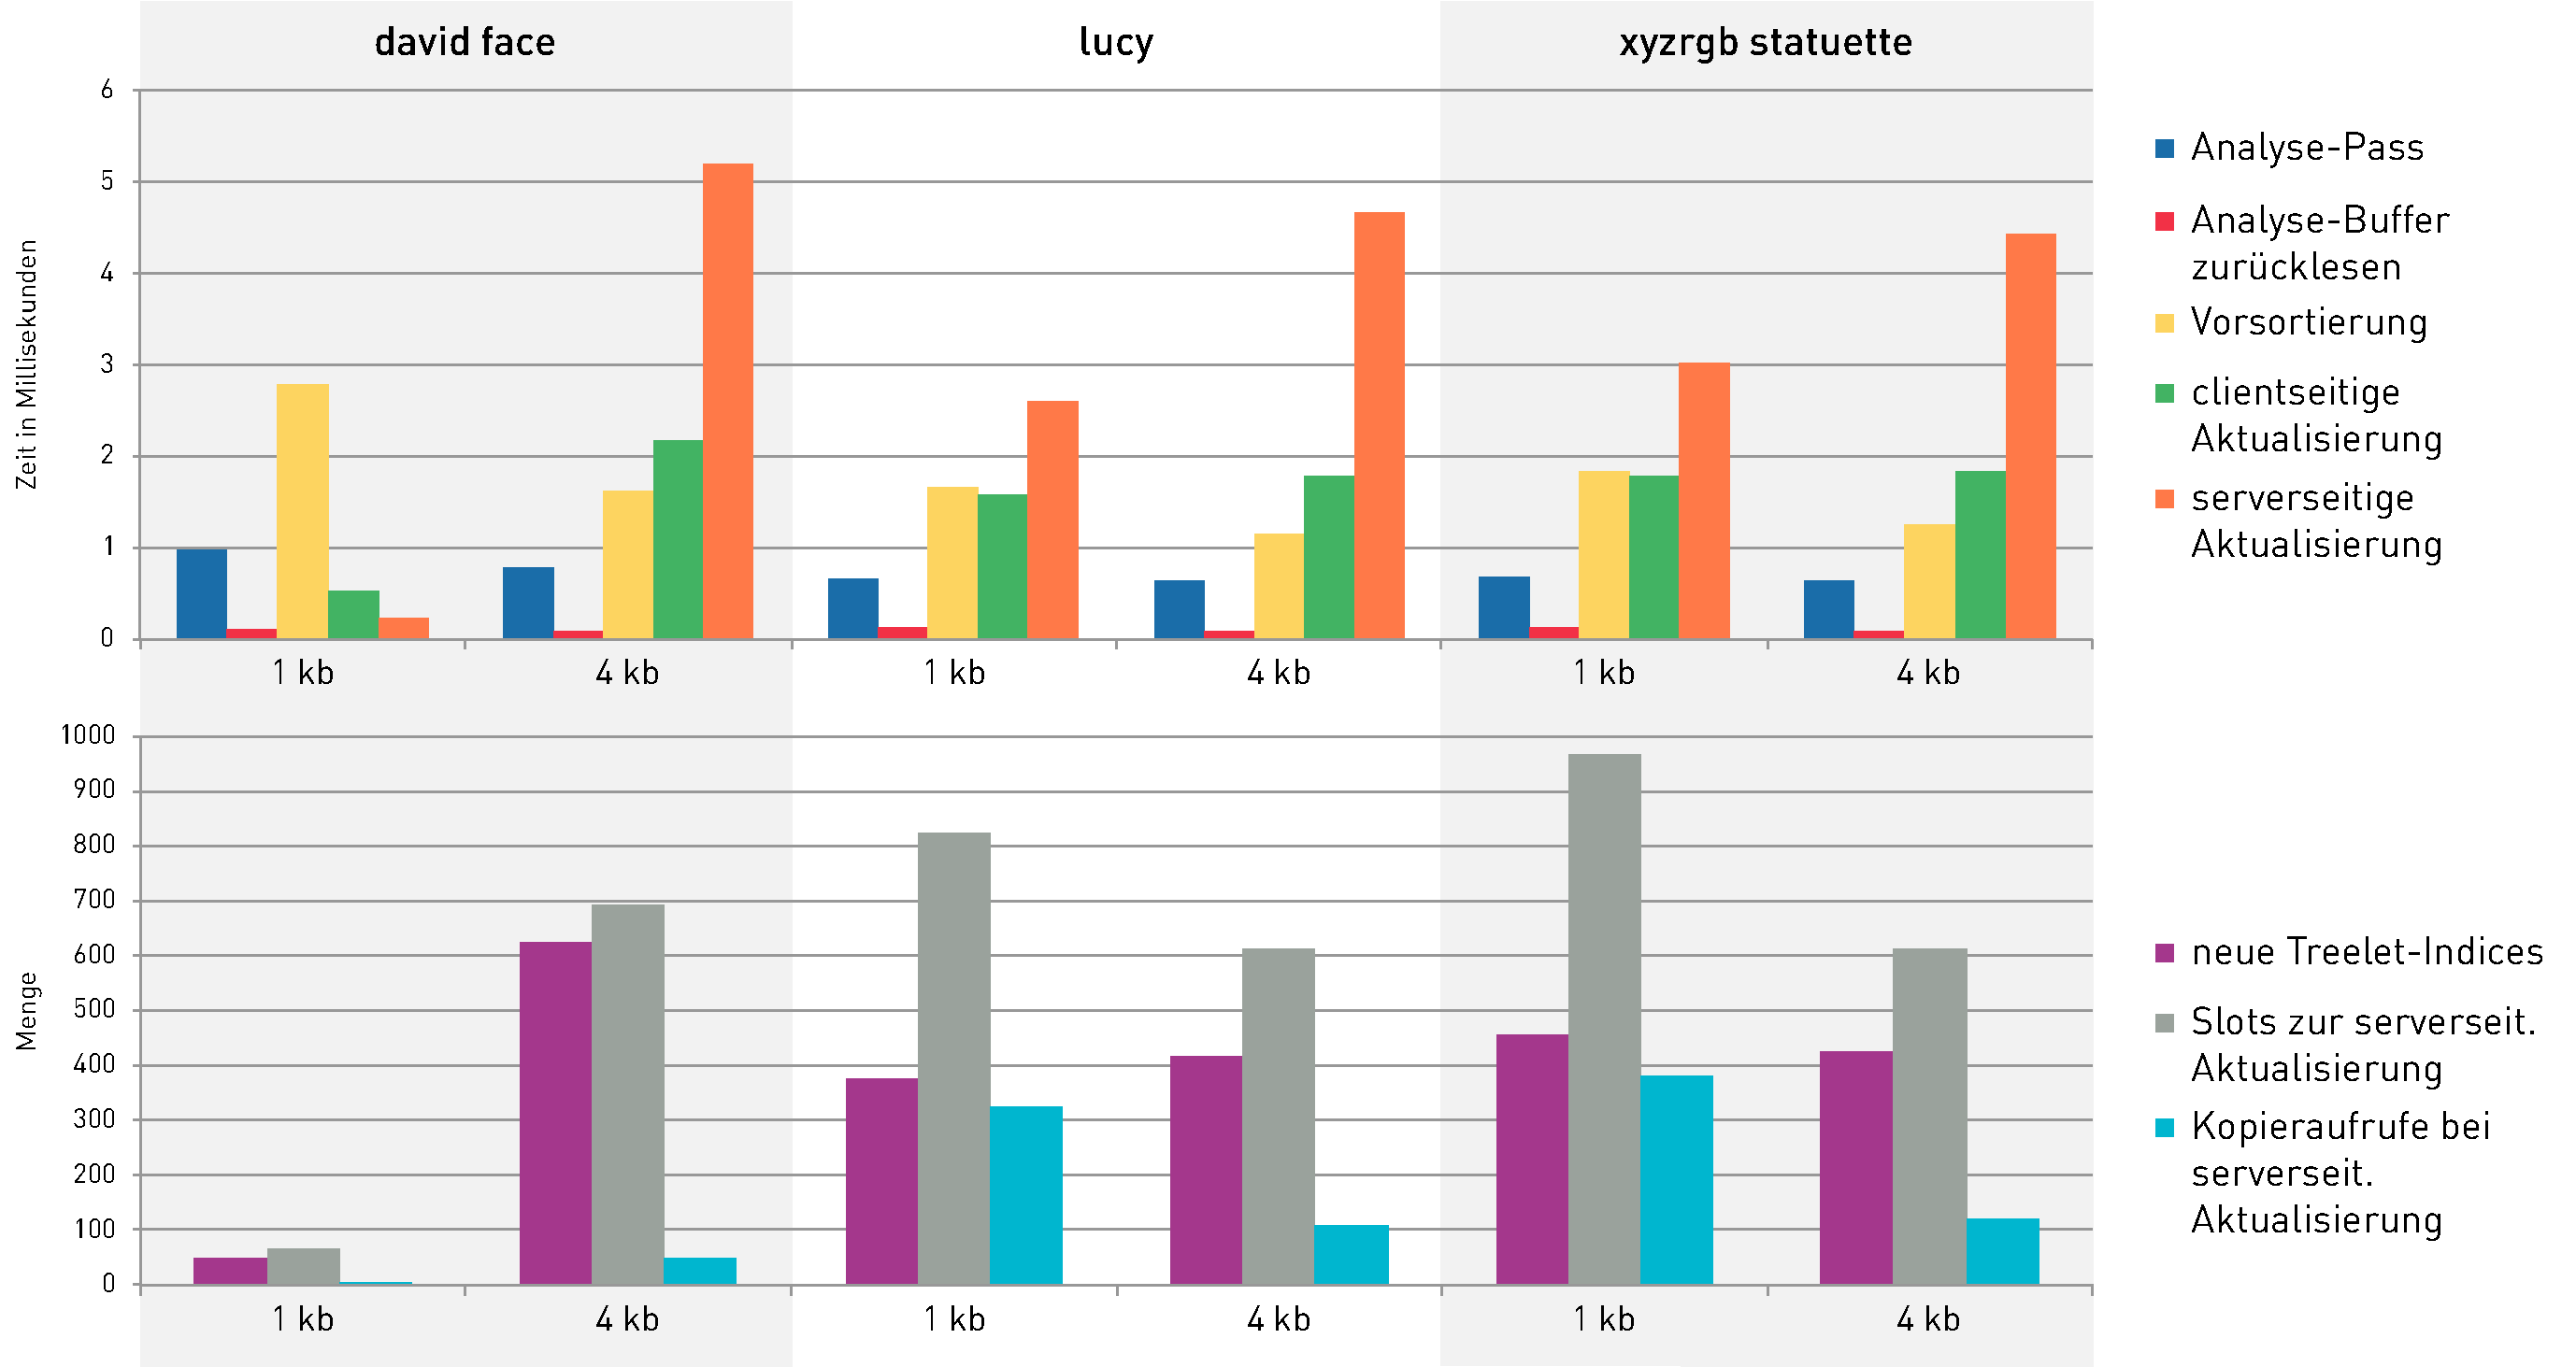
\includegraphics[width=1.0\textwidth]{figures/david_lucy_xyzrgb_s1_vs_24_D13.pdf}
  \caption{Gegen�berstellung von unterschiedlichen Treelet-Gr��en\label{david_lucy_xyzrgb_s1_vs_24_D13}}
\end{figure}

\subsubsection{Erstellung und �bertragung des Analyse-Buffers}
Zun�chst kann festgestellt werden, dass die Erstellungszeit f�r den Analyse-Buffer f�r zwei der drei Beispiele in beiden Treelet-Varianten ann�hernd konstant ist. Der Unterschied beim Modell \textit{david face} kann durch den enormen Unterschied in der Anzahl der Knoten beider Darstellungen erkl�rt werden. Der gr��ere Octree enth�lt die 2.6-fache Menge an Knoten im Vergleich zum kleineren Octree. Trotzdem ben�tigt die 4 Kb Version nur ca. 0.2 ms mehr f�r das Erstellen des Buffers. Daraus l��t sich schlie�en, dass die Gr��e der Treelets f�r die gew�hlten Werte von 1 kB und 4 kB keinen nennens\-werten Einfluss auf das beim Erstellen stattfindende Raycasting besitzt. Daraus kann abgeleitet werden, dass der Algorithmus, trotz der Segmentierung, gut skaliert.\\
Die n�tige �bertragung des Analyse-Buffers in den Hauptspeicher der CPU l�uft erwartungsgem�� in konstanter Zeit ab.

\subsubsection{Vorsortierung}
Der Vorsortierungsschritt ben�tigt bei allen drei Modellen f�r die Variante mit kleinen Treelets mehr Zeit als f�r die Darstellungen mit 4 kB gro�en Treelets. Der Grund f�r dieses Ergebnis ist der gr��ere Verwaltungsaufwand bei der Erstellung der Sicht\-information und Anfragen nach neuen Treelets. Bei\-spiels\-weise muss bei der Behandlung eines Elementes des Analysebuffers das einen Knoten getroffen hat, die Sichtbarkeit des entsprechenden Treelets bis zum Wurzel-Treelet propagiert werden. Falls ein Treelet angehangen werden kann, wird der entsprechende Index mit dem Fehlerwert f�r diesen Bildpunkt in den Container mit allen Treelet-Anfragen sortiert um sie, ihrem Beitrag zur Bildqualit�t nach, ein\-pfle\-gen zu k�nnen.\\
Da die Unterteilung bei 1 kB gro�en Treelets feiner ist, ist auch der Weg zum Propagieren der Sichtbarkeitsinformationen l�nger. Auch ist der Vorgang bei kleinen Treelets wenig speicher\-koh�rent, da es wesentlich mehr Bl�tter und damit mehr Wege von den Bl�ttern zum Wurzel\-knoten gibt. Die feinere Unterteilung f�hrt beim zweiten und dritten Testmodell (\textit{lucy} und \textit{xyzrgb statuette}) zu einer gr��eren Menge von Anfragen nach neuen Treelets.

\subsubsection{Clientseitige Aktualisierung}
Im zweiten und dritten Beispiel (\textit{lucy} und \textit{xyzrgb statuette}) sind die Zeiten f�r die Aktualisierung des clientseitigen Incore-Buffers (obere Graphen, gr�n) nahezu identisch, obwohl sich die Anzahl der vorhandenen Treelets zwischen den der Modellen stark unterscheidet. Die gr��ere Anzahl von Slot-�nderungen (untere Graphen, grau) weist auf eine erh�hte Last bei der Verwaltung der Treelets hin. Besonders beim Modell \textit{lucy} mit 1 kB Treelets wird dies sichtbar, da es deutlich mehr Treelets enth�lt als die anderen drei Octrees. Daraus kann abgeleitet werden, dass die clientseitge Aktualisierung mit steigender Treelet-Anzahl gut skaliert. Allerdings l�sst sich �ber alle Modelle eine st�rkere Abh�ngigkeit der Laufzeit von der Anzahl der neu angeforderten Treelets (untere Graphen, lila) erkennen.

\newpage

\subsubsection{Serverseitige Aktualisierung}
Das Kopieren der ge�nderten Slot-Bereiche auf den Server beansprucht bei fast allen Versuchen einen gro�en Anteil der Laufzeit. Das Zusammenfassen der Slot-Bereiche reduziert die Anzahl von Kopieraufrufe, wie ein Vergleich der Anzahl der ge�nderten Slots (unterer Graph, grau) mit der Anzahl der ausgef�hrten Kopieroperationen (unterer Graph, blau) veranschaulicht. Ob die Zusammenfassung tats�chlich einen Geschwindigkeitsvorteil gegen�ber dem einzelnen Kopieren der Slot-Bereiche bringt, wurde in einem weiteren Test untersucht, der in Abschnitt \ref{sec:test_zusammenfassen_von_slots} (\textit{\nameref{sec:test_zusammenfassen_von_slots}}) dokumentiert ist.

\subsubsection{Einfluss der Treeletgr��e}
Das Modell \textit{david face} stellt eine Besonderheit unter den ausgew�hlten Testmodellen dar. Durch die Segmentierung mit 4 kB gro�en Treelets sind sehr viele Knoten entstanden, die unterhalb der geforderten Tiefe liegen. Dies passiert beim Aufbau der Octree-Struktur im Build-Manager, wenn die gew�nschte Octree-Tiefe mit den bisher erstellten Treelets beinahe erreicht wurde. Auf Voxel-Ebene w�rde es gen�gen, noch einige wenige Unterteilungen vorzunehmen, um die ben�tigte Tiefe zu erreichen. Da aber f�r jeden Blattknoten des bisher erstellten Octrees neue Treelets von 4 kB Gr��e erzeugt werden, wird die Gesamtstruktur sehr gro�. Anders ausgedr�ckt, will man einen Schnitt in der Tiefe 13 durch einen beliebig tiefen Octree abbilden, gelingt das mit 4 kB gro�en Segmenten f�r dieses Modell nur verh�ltnism��ig grob. Damit offenbart sich ein bedeutender Nachteil einer festen Segmentgr��e. Die m�gliche Anzahl von Knoten, deren Tiefe die geforderte minimale Baumtiefe �bersteigt, erh�ht sich mit jeder zus�tzlichen Tiefenstufe, da die Anzahl der Blattknoten gr��er wird.\\
Vergleicht man die in den Graphen dargestellten Werte beider Modellvarianten lassen sich weitere R�ck\-schl�s\-se auf das Verhalten des Systems ziehen. Beispielsweise l�sst sich feststellen, dass das System bei der Darstellung des Modells mit 1 kB gro�en Treelets kaum neue Treelets anfordert (unterer Graph, lila) und somit kaum �nderungen im clientseitigen Incore-Buffer erzeugt (unterer Graph, grau). Dagegen forderte die Modellvariante mit 4 kB gro�en Treelets fortw�hrend neue Treelets zur Anpassung an die aktuelle Ansicht an. Dies ist durch den Gr��enunterschied beider Modelle zu erkl�ren. Die Modell\-variante mit 1 kB gro�en Treelets ist mit 1.4 GB wesentlich gr��er ist als der Incore-Buffer. Trotzdem gelingt es dem System einen Gro�teil der SVO-Struktur im Incore-Buffer zu halten, der f�r das Umfahren des Modells auf einer Achse ben�tigt wird. Nur ein sehr kleiner Teil der Daten, die ben�tigt werden um alle Ansichten der bewegten Kamera optimal aufzul�sen, passt nicht mehr in den Incore-Buffer und wird st�ndig angefordert. Die resultierenden �nderungen in der Belegung des Incore-Buffers scheint sich nur auf einen sehr kleinen, zusammenh�ngenden Bereich zu beschr�nken. Dies kann anhand des Verh�ltnisses der Anzahl an ge�nderten Slot-Bereichen (unterer Graph, grau) und der Anzahl der durchgef�hrten Kopieroperationen (unterer Graph, blau) und anhand der, f�r das Kopieren der Slots ben�tigten Zeit (oberer Graph, orange) erkannt werden.\\
Noch deutlicher wird dies beim Betrachten der Modellvariante mt 4 kB gro�en Treelets. Die Octree-Repr�sentation mit 3.7 GB �bersteigt die Kapazit�t des Incore-Buffers um ein Vielfaches. Hier muss der Octree st�ndig an die aktuelle Ansicht angepasst werden, da zu jedem Zeitpunkt nur die Teile im Incore-Buffer gehalten werden k�nnen, die f�r die aktuelle Ansicht ben�tigt werden. Anhand der Menge angefragter Treelets, der Anzahl von ge�nderten Slot-Positionen und der wenigen Kopieroperationen l�sst sich erkennen, dass immer gro�e, zusammenh�ngende Teile des Incore-Buffers ausgetauscht werden.\\
Die Datenmenge die theoretisch ben�tigt wird, um beide Modellvarianten bis in die, f�r die Ansichten ben�tigte Tiefe abzubilden, ist f�r beide Varianten gleich. Der tats�chlich ben�tigte Schnitt durch den Octree kann vom System jedoch genauer mit kleinen Treelets abgebildet werden. Der pr�zisiere Schnitt durch den Baum f�hrt wiederum zu einer Verbesserung der Gesamtlaufzeit. Dies l�sst sich auch in den Messergebnissen der anderen Modelle feststellen. Selbst beim Modell \textit{lucy}, dessen Repr�sentation mit 1 kB gro�en Treelets deutlich mehr Knoten besitzt, als die Variante mit 4 kB gro�en Treelets, kann eine bessere Gesamt\-leistung festgestellt werden. Mit der gr��eren Anzahl von Treelets steigt jedoch in allen drei Beispielen der Verwaltungsaufwand bei der Vorsortierung (oberer Graph, gelb). Wird die Gr��e der Treelets zu klein, kann der Verwaltungsaufwand f�r die vielen Treelets den Geschwindigkeitsvorteil durch einen besser abbildbaren Schnitt im Baum zunichte machen. Die optimale Treelet-Gr��e in Abh�ngigkeit vom verwendeten Modell sollte in weiteren Tests untersucht werden.


% /////////////////////////////////////////////////////////////

\section{Zusammenfassen von Slots bei der serverseitigen \\Aktualisierung}\label{sec:test_zusammenfassen_von_slots}

Ein gro�er Teil der Laufzeit des Out-of-Core-Systems wird vom Aktualisieren des serverseitigen Incore-Buffers beansprucht. Daher h�tte eine Optimierung dieses Vorgangs einen gro�en Einfluss auf die Gesamt\-leistung des Systems. Es wurde zun�chst vermutet, dass die gro�e Anzahl der Kopier\-operationen vom clientseitigen zum serverseitigen Incore-Buffer f�r den Gro�teil der ben�tigten Zeit verantwortlich ist. Mit dem Zusammenfassen der Speicherbereiche mehrerer Slots wurde versucht, die Anzahl der Kopieroperationen zu minimieren. Der festgelegte Anteil der Nutzdaten an dem zu kopierenden Speicher\-be\-reich wirkt sich dabei entscheidend auf die ben�tigte Laufzeit aus. Ist der Anteil zu hoch k�nnen nur wenige Be\-reiche zusammengefasst werden. Ist er dagegen zu niedrig, wird im Extremfall der Be\-reich des gesamten Incore-Buffers zu einer Kopieroperation zusammengefasst. Zum �bertragen einer so gro�en Datenmenge w�rde mehr Zeit ben�tigt werden, als bei der Einzel\-�bertragung der Slot-Bereiche. Es muss also einen Wert f�r den Anteil von Nutzdaten geben, bei dem die ben�tigte Zeit f�r das Kopieren minimiert wird. Dieser Test wurde durchgef�hrt um diesen Wert f�r eine gegebene Konfiguration von Incore-Buffer-Gr��e und Eingabedaten zu finden.


\subsection{Versuchsaufbau}
Das Modell \textit{david face} mit 4 kB gro�en Treelets wurde analog zum ersten Test vor der Kamera bewegt. In zehn Durchl�ufen wurden zeitlicher Aufwand f�r die serverseitige Aktualisierung, die Menge der ver�nderten Slots und die Anzahl der ausgef�hrten Kopieroperationen �ber eine Dauer von 30 Sekunden aufgezeichnet. Dabei wurde der geforderte Nutzdatenanteil in jedem Durchlauf mit 0 beginnend, um 0.1 bis zu einem Wert von 1 erh�ht. Um Artefakte in den gemessenen Werten zu verhindern, wurde das Modell wie im vorherigen Test �ber 30 Sekunden aus zuf�llig gew�hlten Perspektiven verarbeitet, bevor mit den Messungen begonnen wurde.


\subsection{Auswertung}
Abbildung \ref{ratio_0_1} zeigt die Zeit f�r die serverseitige Aktualisierung, die Anzahl von ge�nderten Slots und die Menge von durchgef�hrten Kopieroperationen. Dabei besagt ein Anteil von 0, dass kopierte Bereiche keine Nutzdaten enthalten m�ssen. Ein Anteil von 1 bedeutet dagegen, dass jeder in einem zu kopierenden Bereich liegender Slot auch ge�nderte Daten enhalten muss. In der Abbildung l�sst sich ein Optimum f�r einen Nutzdatenanteil von 0.6 erkennen. Mit dieser Einstellung betrug die Zeit f�r die �bertragung im Durchschnitt 2.48 ms. Zum Vergleich lag die Zeit f�r das separate Kopieren einzelner Slots im Durchschnitt bei 4.23 ms. Der im Graph nicht sichtbare Wert f�r einen Nutzdatenanteil von 0 lag bei 52.51 ms.\\
Ein Optimum scheint also zu existieren. Wie sich der Wert jedoch im laufenden System �ndert und wie er von anderen Systemparametern abh�ngt, wurde im Zuge dieser Arbeit nicht untersucht.


\begin{figure}[position=h]
  \centering
  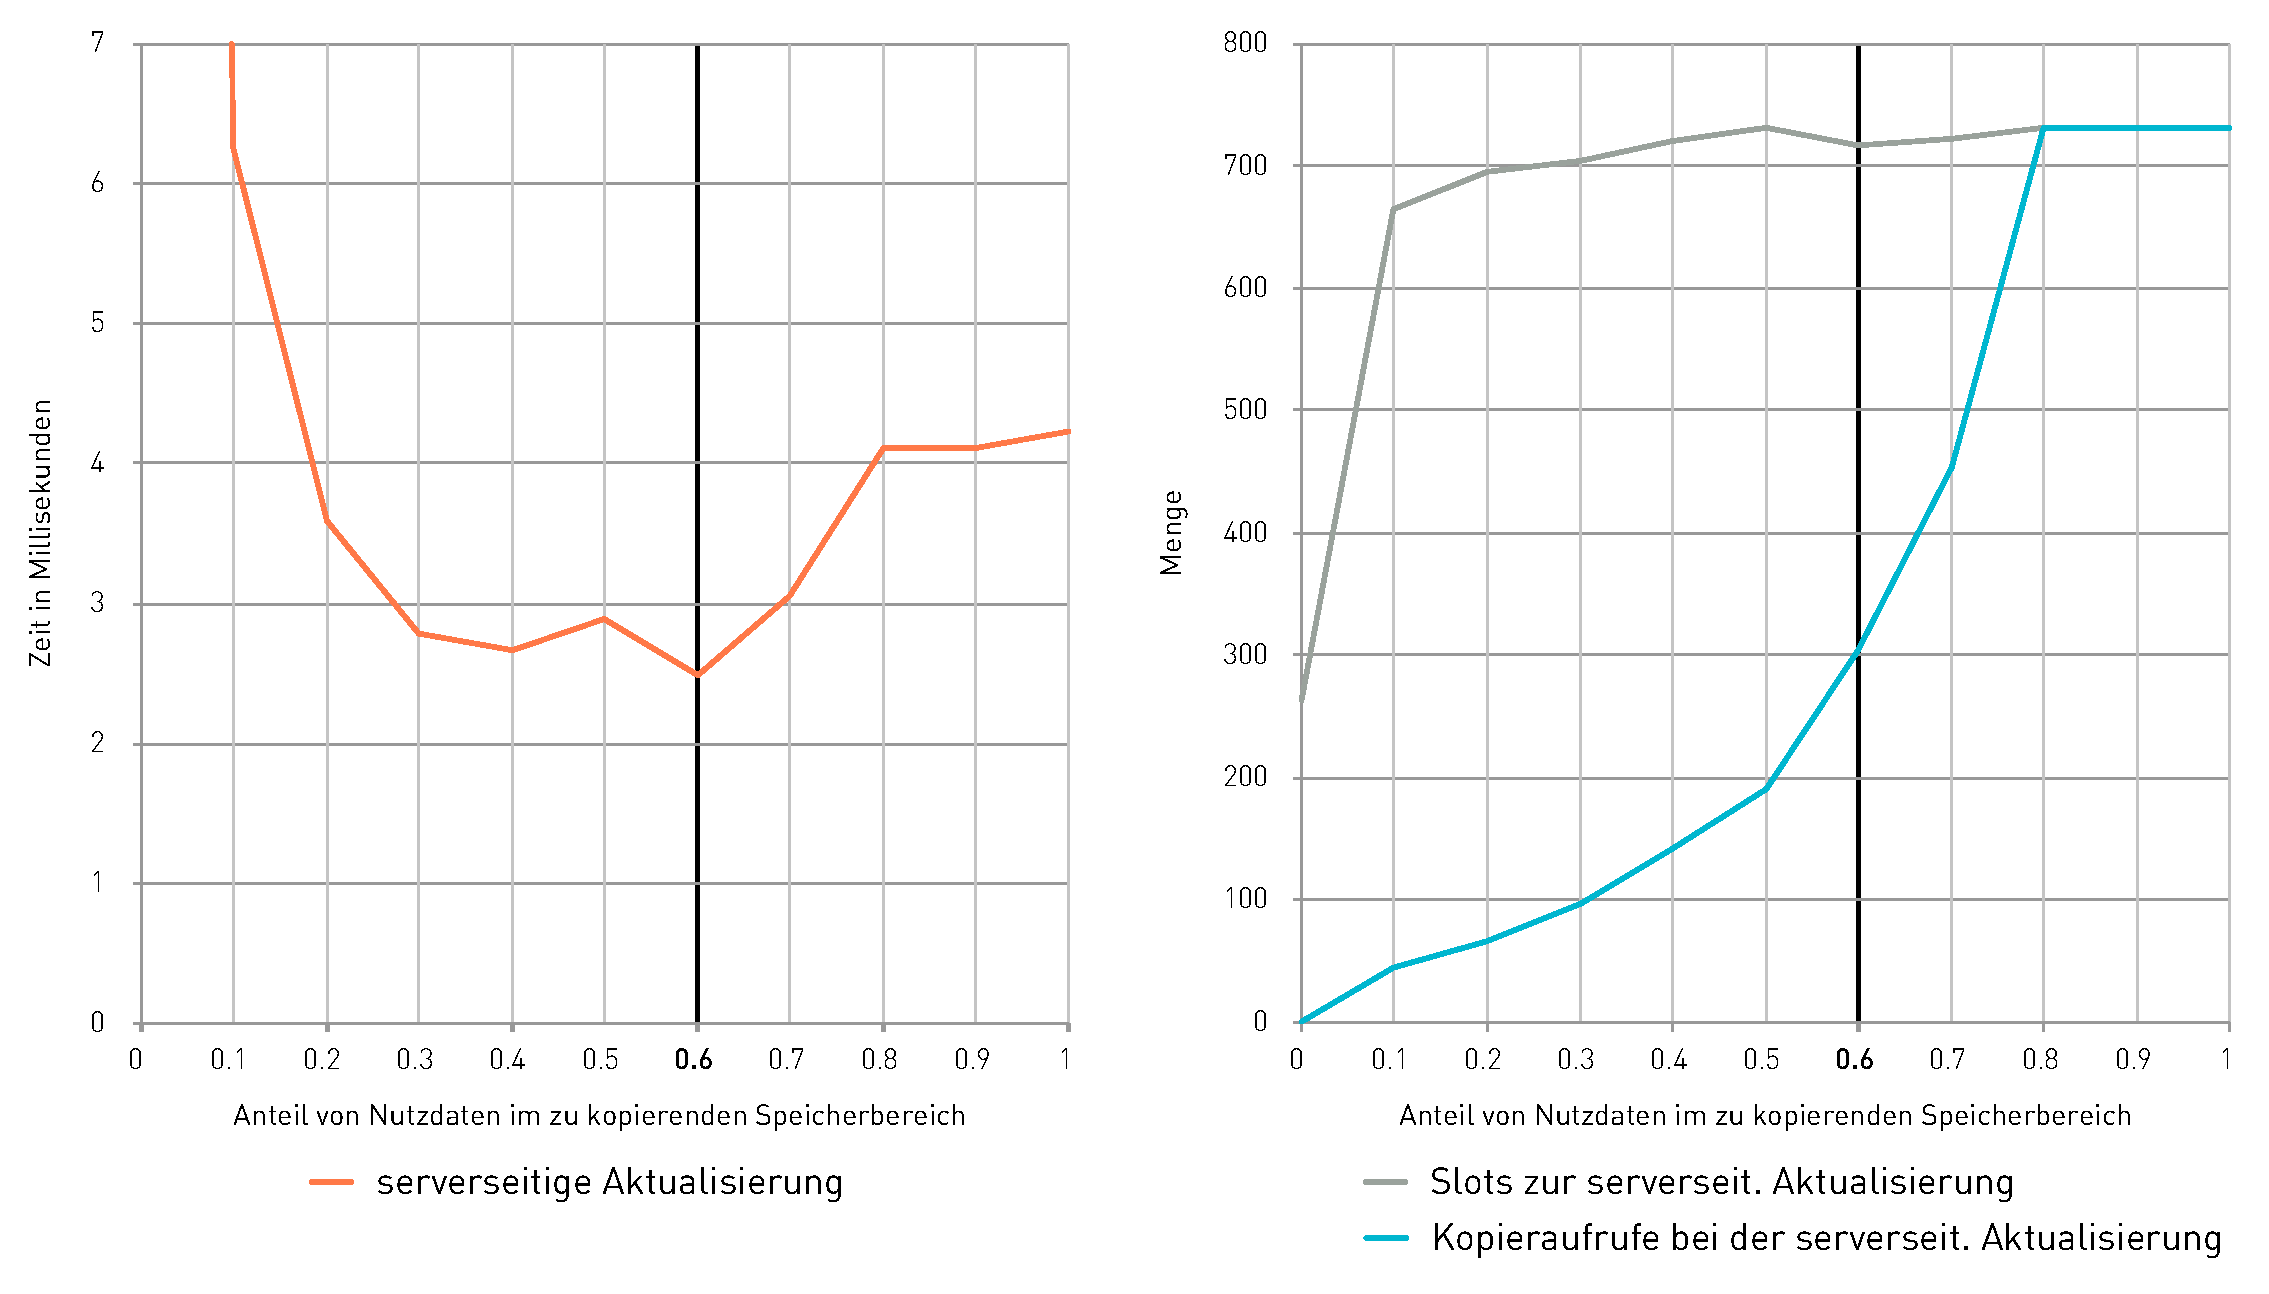
\includegraphics[width=1.0\textwidth]{figures/ratio_0-1.pdf}
  \caption{Idealwert f�r Nutzdatenanteil\label{ratio_0_1}}
\end{figure}


% /////////////////////////////////////////////////////////////

\newpage
\section{Test der Reaktionsf�higkeit des Systems}

In diesem Versuch soll die Reaktionsf�higkeit des Systems untersucht. Dazu wurde die Zeit gemessen, die das System ben�tigt um auf eine Sichtver�nderung zu reagieren, indem es den aktuell sichtbaren Teil des Octrees bis zum n�tigen, beziehungsweise m�glichen Grad, verfeinert. Die Anzahl der zur Verfeinerung angeforderten Treelets kann dabei als Fehlerwert, f�r den momentan im Incore-Buffer befindlichen Teil des Octrees, im Vergleich zu einem f�r diese Ansicht optimalen Octree, gesehen werden.


\subsection{Versuchsaufbau}

F�r diesen Test wurde die Kamera zun�chst auf das Modell gerichtet und dann die Verfeinerung des Octrees aktiviert. Nachdem die Verfeinerung f�r diese Ansicht abgeschlossen war, wurde die Kamera schnell auf das Modell zu bewegt, um davor wieder zum Stehen zu kommen. Nachdem die Verfeinerung des Octrees f�r diese Ansicht abgeschlossen war, wurde das Modell noch einmal in einer schnellen Bewegung umkreist. W�hrend dieses Ablaufs wurden Werte f�r die Kamerageschwindigkeit, die ben�tigte Zeit f�r die Bildsynthese und den Gesamtzyklus, sowie f�r die Anzahl der angeforderten Treelets aufgezeichnet. Der Bewegungsablauf soll das Verhalten eines Betrachters simulieren.


\subsection{Auswertung}
Die in Abschnitt \ref{sec:streaming_vorsortierung} \textit{\nameref{sec:streaming_vorsortierung}} besprochene Anordnung der Treelet-Anfragen spielt f�r die Be\-wert\-ung der Ergebnisse dieses Versuches eine wichtige Rolle. Die Sortierung der Anfragen nach ihrem Fehler in der Darstellung sorgt daf�r, dass zuerst diejenigen Treelets eingepflegt werden, die den gr��ten Beitrag zur Darstellungs\-qualit�t liefern. Somit finden Verfeinerungen von groben Strukturen zuerst statt, w�hrend im sp�teren Verlauf der Verfeinerung einer Ansicht die Darstellungs\-qualit�t nur noch unbedeutend steigt. Das in Abschnitt \ref{sec:streaming_analyse_pass} {\nameref{sec:streaming_analyse_pass} beschriebene Verfahren f�hrt dazu, dass die Verfeinerung nie abgeschlossen ist, da bedingt durch die Unterabtastung beim F�llen des Analyse-Buffers immer wieder Blatt\-knoten getroffen werden, die in keinem vorherigen Analyse-Pass sichtbar waren. Knoten, die vom Analyse-Pass lange unentdeckt bleiben, sind meist klein. Daher ist auch ihr Beitrag zur Bild\-qualit�t vernachl�ssigbar klein. Abbildung \ref{progressive_refinement} zeigt die Verfeinerung einer Ansicht in f�nf auf\-einander\-folgenden Schritten.

\begin{figure}[H]
  \centering
  \includegraphics[width=0.9\textwidth]{figures/progressive_refinement.png}
  \caption{Verfeinerung f�r eine Ansicht in f�nf Schritten\label{progressive_refinement}}
\end{figure}

Der Darstellungs\-fehler ist in der unteren Reihe auf einen Farbverlauf von Gr�n �ber Gelb nach Rot abgebildet. Die Abbildungen lassen erkennen, dass die Verfeinerung bereits nach wenigen Schritten so weit vorangeschritten ist, dass die weiterhin stattfindende Verfeinerung kaum noch zur wahr\-ge\-nommenen Bildqualit�t beitr�gt.


Abbildung \ref{kamera_fahrt} zeigt die Ergebnisse der durchgef�hrten Messung und die aufgenommenen Werte im zeitlichen Verlauf. Von Zeitpunkt Null an beginnt die Verfeinerung der Octree-Struktur und ist nach etwa 3.5 Sekunden praktisch abgeschlossen. Nach vier Sekunden beginnt die Kamera\-bewegung in Richtung Modell, welche nach weiteren f�nf Sekunden beendet ist. In dieser Zeit steigt die f�r die Bildsynthese ben�tigte Zeit deutlich an. Dies ist dadurch bedingt, dass durch die wachsende Fl�che des abgebildeten Modells im Bildausschnitt beim Raycasting mehr Strahlen den Octree traversieren m�ssen. Bei 6 Sekunden beginnt die Verfeinerung weiter voranzuschreiten, da die Tiefe der geladenen Treelets nicht mehr f�r die Darstellung des Modells in dieser Entfernung ausreicht. Vier Sekunden nach der Beendigung der Kamerabewegung ist die Menge der angefordeten Treelets wieder auf einen sehr geringen Wert ge\-fal\-len. Abbildung \ref{difference} zeigt das Bild w�hrend des Testdurchlaufs zum Zeitpunkt 8.5 Sekunden (links) und 12.5 Sekunden (mitte). Im Differenzbild (rechts) ist deutlich zu erkennen wie gering der Beitrag der eingepflegten f�r die Darstellungsqualit�t ist. Es handelt sich dabei meist um pixel-gro�e Bereiche. Ihre Anordnung im Differenzbild zeigt deutliche Aliasingartefakte in Form von regelm��igen Mustern, was auf die Arbeitsweise des Analyse-Passes zur�ckgef�hrt werden kann. 

\begin{figure}[position=h]
  \centering
  \includegraphics[width=1.0\textwidth]{figures/difference.png}
  \caption{Unterschiede der Verfeinerung zu zwei Zeitpunken\label{difference}}
\end{figure}

In der 13. Sekunde beginnt die umkreisende Bewegung der Kamera, die zu einem deutlichen Anstieg der Menge der angeforderten Treelets f�hrt. Bei 18.5 Sekunden ist die Umkreisung so weit vorangeschritten, dass wieder Bereiche des Modells dargestellt werden, die im bisherigen Verlauf des Test schon sichtbar waren. Damit sinkt auch die Menge der angeforderten Treelets. Bei 22.5 Sekunden beginnt die Menge der angeforderten Treelets wieder zu steigen. Der Grund f�r den Anstieg ist, dass die f�r die Frontansicht des Modells ben�tigten Treelets bereits aus dem Incore-Buffer verdr�ngt wurden.\\
Drei Sekunden nach Beendigung der Umkreisung war die, im Incore-Buffer enthaltene Octree-Struktur erneut an die Ansicht angepasst.\\
\\
Der Test zeigt, dass das vorgestellte Out-of-Core-System schnell auf Ver�nderungen der Ansicht mit �nderungen der Auswahl der Octree-Segmente reagieren kann. Die mit dem System erzielte Bildrate lag im Test meist �ber 50 Hz. Dabei wurden Out-of-Core-System und Bildgenerierung durch Raycasting sequentiell ausgef�hrt. Die Aufl�sung des Bild-Buffers in diesem Test betrug 1024x1024 Pixel.

\begin{figure}[position=h]
  \centering
  \includegraphics[width=1.0\textwidth]{figures/kamera_fahrt.pdf}
  \caption{Reaktionszeit des Systems\label{kamera_fahrt}}
\end{figure}

% /////////////////////////////////////////////////////////////


\newpage
\chapter{Zusammenfassung und Ausblick}


\section{Zusammenfassung}

%Der Schwerpunkt der vorliegende Arbeit liegt auf...

In der vorliegende Arbeit wurde ein Out-of-Core Ansatz zur Darstellung von gro�en Sparse Voxel Octree Strukturen entwickelt. Dieser arbeitet durch Segmentierung der Octree-Daten in Teile fester Gr��e. Die Anpassung der darzustellenden Untermenge an Octree-Daten wurde durch ein Analysesystem realisiert das auf Abtastung der momentan vorgehaltenen Daten basiert.



Zur Erstellung von Inhalten wurde ein generalisiertes System zur Erstellung von Sparse Voxel Octrees aus unterschiedlichen Ausgangsformaten entworfen. Um die Ergebnisse der Erstellung und des Out-of-Core-Ansatzes zu validieren wurde der Raycasting-Algorithmus in OpenCL implementiert.\\
\\
Es konnte gezeigt werden, dass sich mit dem vorgestellten Out-of-Core-Ansatz eine schnelle Anpassung der Darstellung des Octrees an die Ansicht des Betrachters m�glich ist. 


Die Tests haben gezeigt ... 


\section{Ausblick}



%\newpage
%\input{Ausblick/Ausblick.tex}
%\newpage
%\addcontentsline{toc}{chapter}{Literatur}
%\bibliography{literatur}
%\newpage
%\input{Appendix/Appendix.tex}
\end{document}